\section{Specific Requirement}
In this section, it is given a complete description of the functional requirements of the system.
\subsection{Requirements}
\begin{enumerate}[label=\bfseries R\arabic*]
    \item The system must allow  users to register on the platform as educator or student.
    \item The system must allow  users to login.
    \item  The system must enable educators who have created a tournament to grant permissions to other educator  to create battles within that specific tournament.

    
    \item The system must allow the educator to see which tournaments they have permission for.
    \item The system must allow educator to insert information about a tournament.
    \item The system must allow educator to insert information about a battle for the tournament in which he has the permissions.
    
    \item The system must notify via mail subscribed students to the platform upon the creation of new tournaments.
    \item  The system must allow students to subscribe to tournament on the CKB platform before a specific deadline.
    \item  The system must notify via mail  all students subscribed in the tournament whenever a new battle is created within that tournament.

    \item The system must allow students to subscribe in the battle.

    \item The system should enable students to invite other students who do not yet have a team to create a team.
    
    \item The system must notify via mail all students who are invited to form a team.
    \item The system must allow students to accept an invitation via email to join in a team.
    \item The system must allow student to decline the invitation via email to join in a team
    \item The system must notify via mail the team's creator when an invited student declines his invitation.
    \item The system must notify via mail all members of a team when a new student joins their team.

    \item The system must allow user to see the list of available tournaments.
    \item The system must allow user to see the list of available battles.
    
    \item The system must integrate with GitHub for repository management and automate the process of code submission and evaluation.

    \item The system must allow educators who have set manually evaluation to see the submitted projects.
    \item The system must allow educators who have set manually evaluation to upload a manually score for each project. 
    
    \item The system must automatically create a GitHub repository containing the code kata upon the expiration of the battle's registration deadline.
    \item The system must notify via email the link to the repository containing the code kata to all students who are members of a team registered for the battle.
    
    \item The system must automatically pull and analyze the latest sources from student repositories upon each commit.
    
    \item The system must support automated test execution and static analysis of submitted code.
    
    \item The system must calculate battle  scores based on functional aspects, timeliness, and quality level of sources.

    
    \item The system must update battle scores in real-time as students push new commits.
    
    \item The system must consolidate and finalize battle scores after the submission deadline and provide a final battle rank.
    
    \item The system must notify via mail  all students involved in a battle when final battle rank becomes available.

    
    \item The system must calculate and update tournament score at the end of each battle.
    \item The system must create and update the tournament rankings.
    \item The system must create and update the battle rankings in real time.
    
    \item  The system must allow educators with permission on the tournament  to close it. 

    \item  The system must ensure that the final score of each battle for a team falls within the range of 0 to 100.



    \item  The system must allow educators with the necessary permissions to delete a tournament in which no battles are currently ongoing.

    \item  The system must allow educators with necessary permissions to delete a battle  that is not currently ongoing.
    
    \item The system automatically deletes a battle when no teams have subscribed to it by the registration deadline
  


\end{enumerate}
\subsubsection{Mapping between Goal,Domain Assumption and requirements}
This paragraph will show  the mapping between goals described in section 1.1.1 and requirements and  domain assumptions.

\textbf{G1 - Educators can manage coding tournaments and battles.}
\begin{itemize}
    \item [$R01$] The system must allow users to register on the platform as educator or student.
    \item [$R02$]The system must allow users to login.
    \item [$R03$] The system must enable educators who have created a tournament to grant permissions to other
    educator to create battles within that specific tournament.
    \item [$R04$]The system must allow the educator to see which tournaments they have permission for.
    \item [$R05$] The system must allow educator to insert information about a tournament.
    \item [$R06$]The system must allow educator to insert information about a battle for the tournament in which
    he has the permissions.
    \item [$R17$]The system must allow user to see the list of available tournaments.
    \item [$R33$]The system must allow educators with permission on the tournament to close it.
    \item [$R35$] The system must allow educators with the necessary permissions to delete a tournament in which no battles are currently ongoing.
     \item [$R36$]The system must allow educators with necessary permissions to delete a battle  that is not currently ongoing.
      \item [$R37$]The system automatically deletes a battle when no teams have subscribed to it by the registration deadline.
\item [$DA1$]Both educators and students must have an e-mail.
\item [$DA3$] Users who register on the CKB platform in the role of 'educator' are skilled  in designing meaningful and challenging code katas and also in evaluating them.
\item [$DA4$] Users have consistent and reliable access to the internet and the necessary technology to participate in coding battles and tournaments.
   
\end{itemize}
  \textbf{G2 - Students can form teams for coding battles.}
\begin{itemize}
    \item [$R01$] The system must allow users to register on the platform as educator or student.
    \item [$R02$]The system must allow users to login.
    \item [$R11$]  The system should enable students to invite other students who do not yet have a team to create a team.
    \item [$R12$]  The system must notify via mail all students who are invited to form a team.
    \item [$R13$] The system must allow students to accept an invitation via email to join in a team.
     \item [$R14$]The system must allow student to decline the invitation via email to join in a team.
     \item [$R15$]The system must notify via mail the team’s creator when an invited student declines his invitation.
     \item [$R16$] The system must notify via mail all members of a team when a new student joins their team.
    \item [$DA1$] Both educators and students must have an e-mail.
    \item [$DA4$] Users have consistent and reliable access to the internet and the necessary technology (com-
puters, software development tools) to participate in coding battles and tournaments.
   
\end{itemize}

  \textbf{G3 -  Students can participate in coding battles}
\begin{itemize}
 \item [$R01$] The system must allow users to register on the platform as educator or student.
    \item [$R02$]The system must allow users to login.
    \item [$R07$]The system must notify via mail subscribed students to the platform upon the creation of new
tournaments.
    \item [$R08$]The system must allow students to subscribe to tournament on the CKB platform before a specific
deadline.
    \item [$R09$]The system must notify via mail all students subscribed in the tournament whenever a new battle
is created within that tournament.
    \item [$R10$]The system must allow students to subscribe in the battle.
    
    \item [$R18$]  The system must allow user to see the list of available battles.
    \item[$R19$]  The system must integrate with GitHub for repository management and automate the process of
code submission and evaluation.
\item [$R22$] The system must automatically create a GitHub repository containing the code kata upon the
expiration of the battle’s registration deadline
\item [$R23$] The system must notify via email the link to the repository containing the code kata to all students
who are members of a team registered for the battle.
%\item [$R24$]-25 The system must automatically pull and analyze the latest sources from student repositories upon
%each commit. ??
    \item [$DA1$]Both educators and students must have an e-mail.
    \item [$DA2$] Students must have a Github account.
    \item [$DA4$]Users have consistent and reliable access to the internet and the necessary technology (com-
puters, software development tools) to participate in coding battles and tournaments.
    \item [$DA5$] The integration with GitHub and GitHub Actions functions correctly, allowing for seamless
repository management, code submission, and automated workflow for the students’ projects
    \item [$DA6$] Users who register on the CKB platform in the role of ’student’ have familiarity with pro-
gramming languages, GitHub, and test-driven development methodologies.
\end{itemize}
\
 \textbf{G4 -  Educators are able to evaluate manually the projects of the students}
\begin{itemize}
 \item [$R01$] The system must allow users to register on the platform as educator or student.
\item [$R02$]The system must allow users to login.
\item [$R04$]The system must allow the educator to see which tournaments they have permission for.
\item [$R18$]The system must allow user to see the list of available battles.
\item [$R20$]The system must allow educators who have set manually evaluation to see the submitted projects.
\item [$R21$] The system must allow educators who have set manually evaluation to upload a manually score for
each project.
 \item [$R34$] The system must ensure that the final score of each battle for a team falls within the range of 0 to 100.
\item [$DA1$]Both educators and students must have an e-mail.
\item [$DA3$]Users who register on the CKB platform in the role of 'educator' are skilled  in designing meaningful and challenging code katas and also in evaluating them.
\item [$DA4$]Users have consistent and reliable access to the internet and the necessary technology (com-
puters, software development tools) to participate in coding battles and tournaments.
   
\end{itemize}

 \textbf{G5 - Projects are evaluated in an automated way}
\begin{itemize}
\item [$R24$]The system must automatically pull and analyze the latest sources from student repositories upon
each commit
\item [$R25$]The system must support automated test execution and static analysis of submitted code.
\item [$R26$]The system must calculate battle scores based on functional aspects, timeliness, and quality level
of source
 \item [$R34$] The system must ensure that the final score of each battle for a team falls within the range of 0 to 100.
\item[$DA5$]The integration with GitHub and GitHub Actions functions correctly, allowing for seamless
repository management, code submission, and automated workflow for the students’ projects.
\end{itemize}

\textbf{G6 - Educators and students can see the rank of the battles and tournaments}
\begin{itemize}
 \item [$R01$] The system must allow users to register on the platform as educator or student.
\item [$R02$]The system must allow users to login.
\item [$R17$]The system must allow user to see the list of available tournaments.
\item [$R18$]The system must allow user to see the list of available battles.
\item [$R26$]The system must calculate battle scores based on functional aspects, timeliness, and quality level
of sources.
\item [$R27$]The system must update  battle scores in real-time as students push new commits.
\item [$R28$]The system must consolidate and finalize battle scores after the submission deadline and provide
a final battle rank.
\item [$R29$]The system must notify via mail all students involved in a battle when final battle rank becomes
available.
\item [$R30$] The system must calculate and update tournament score at the end of each battle.
\item [$R31$] The system must create and update the tournament rankings
\item [$R32$]The system must create and update the battle rankings in real time.
\item [$DA1$]Both educators and students must have an e-mail.
\item [$DA4$]Users have consistent and reliable access to the internet and the necessary technology (com-
puters, software development tools) to participate in coding battles and tournaments.
\item [$DA5$] The integration with GitHub and GitHub Actions functions correctly, allowing for seamless
repository management, code submission, and automated workflow for the students’ projects
    
   
\end{itemize}

\newpage
\subsection{External interface requirements}
\subsubsection{User interface}
Within this section of the document, we showcase a portion of the CKB web application's user interface (UI). Specifically, we present three interfaces that pertain to the functionalities of Login, Registration, and the Homepage.

 \begin{figure}[H]
  %\centering
  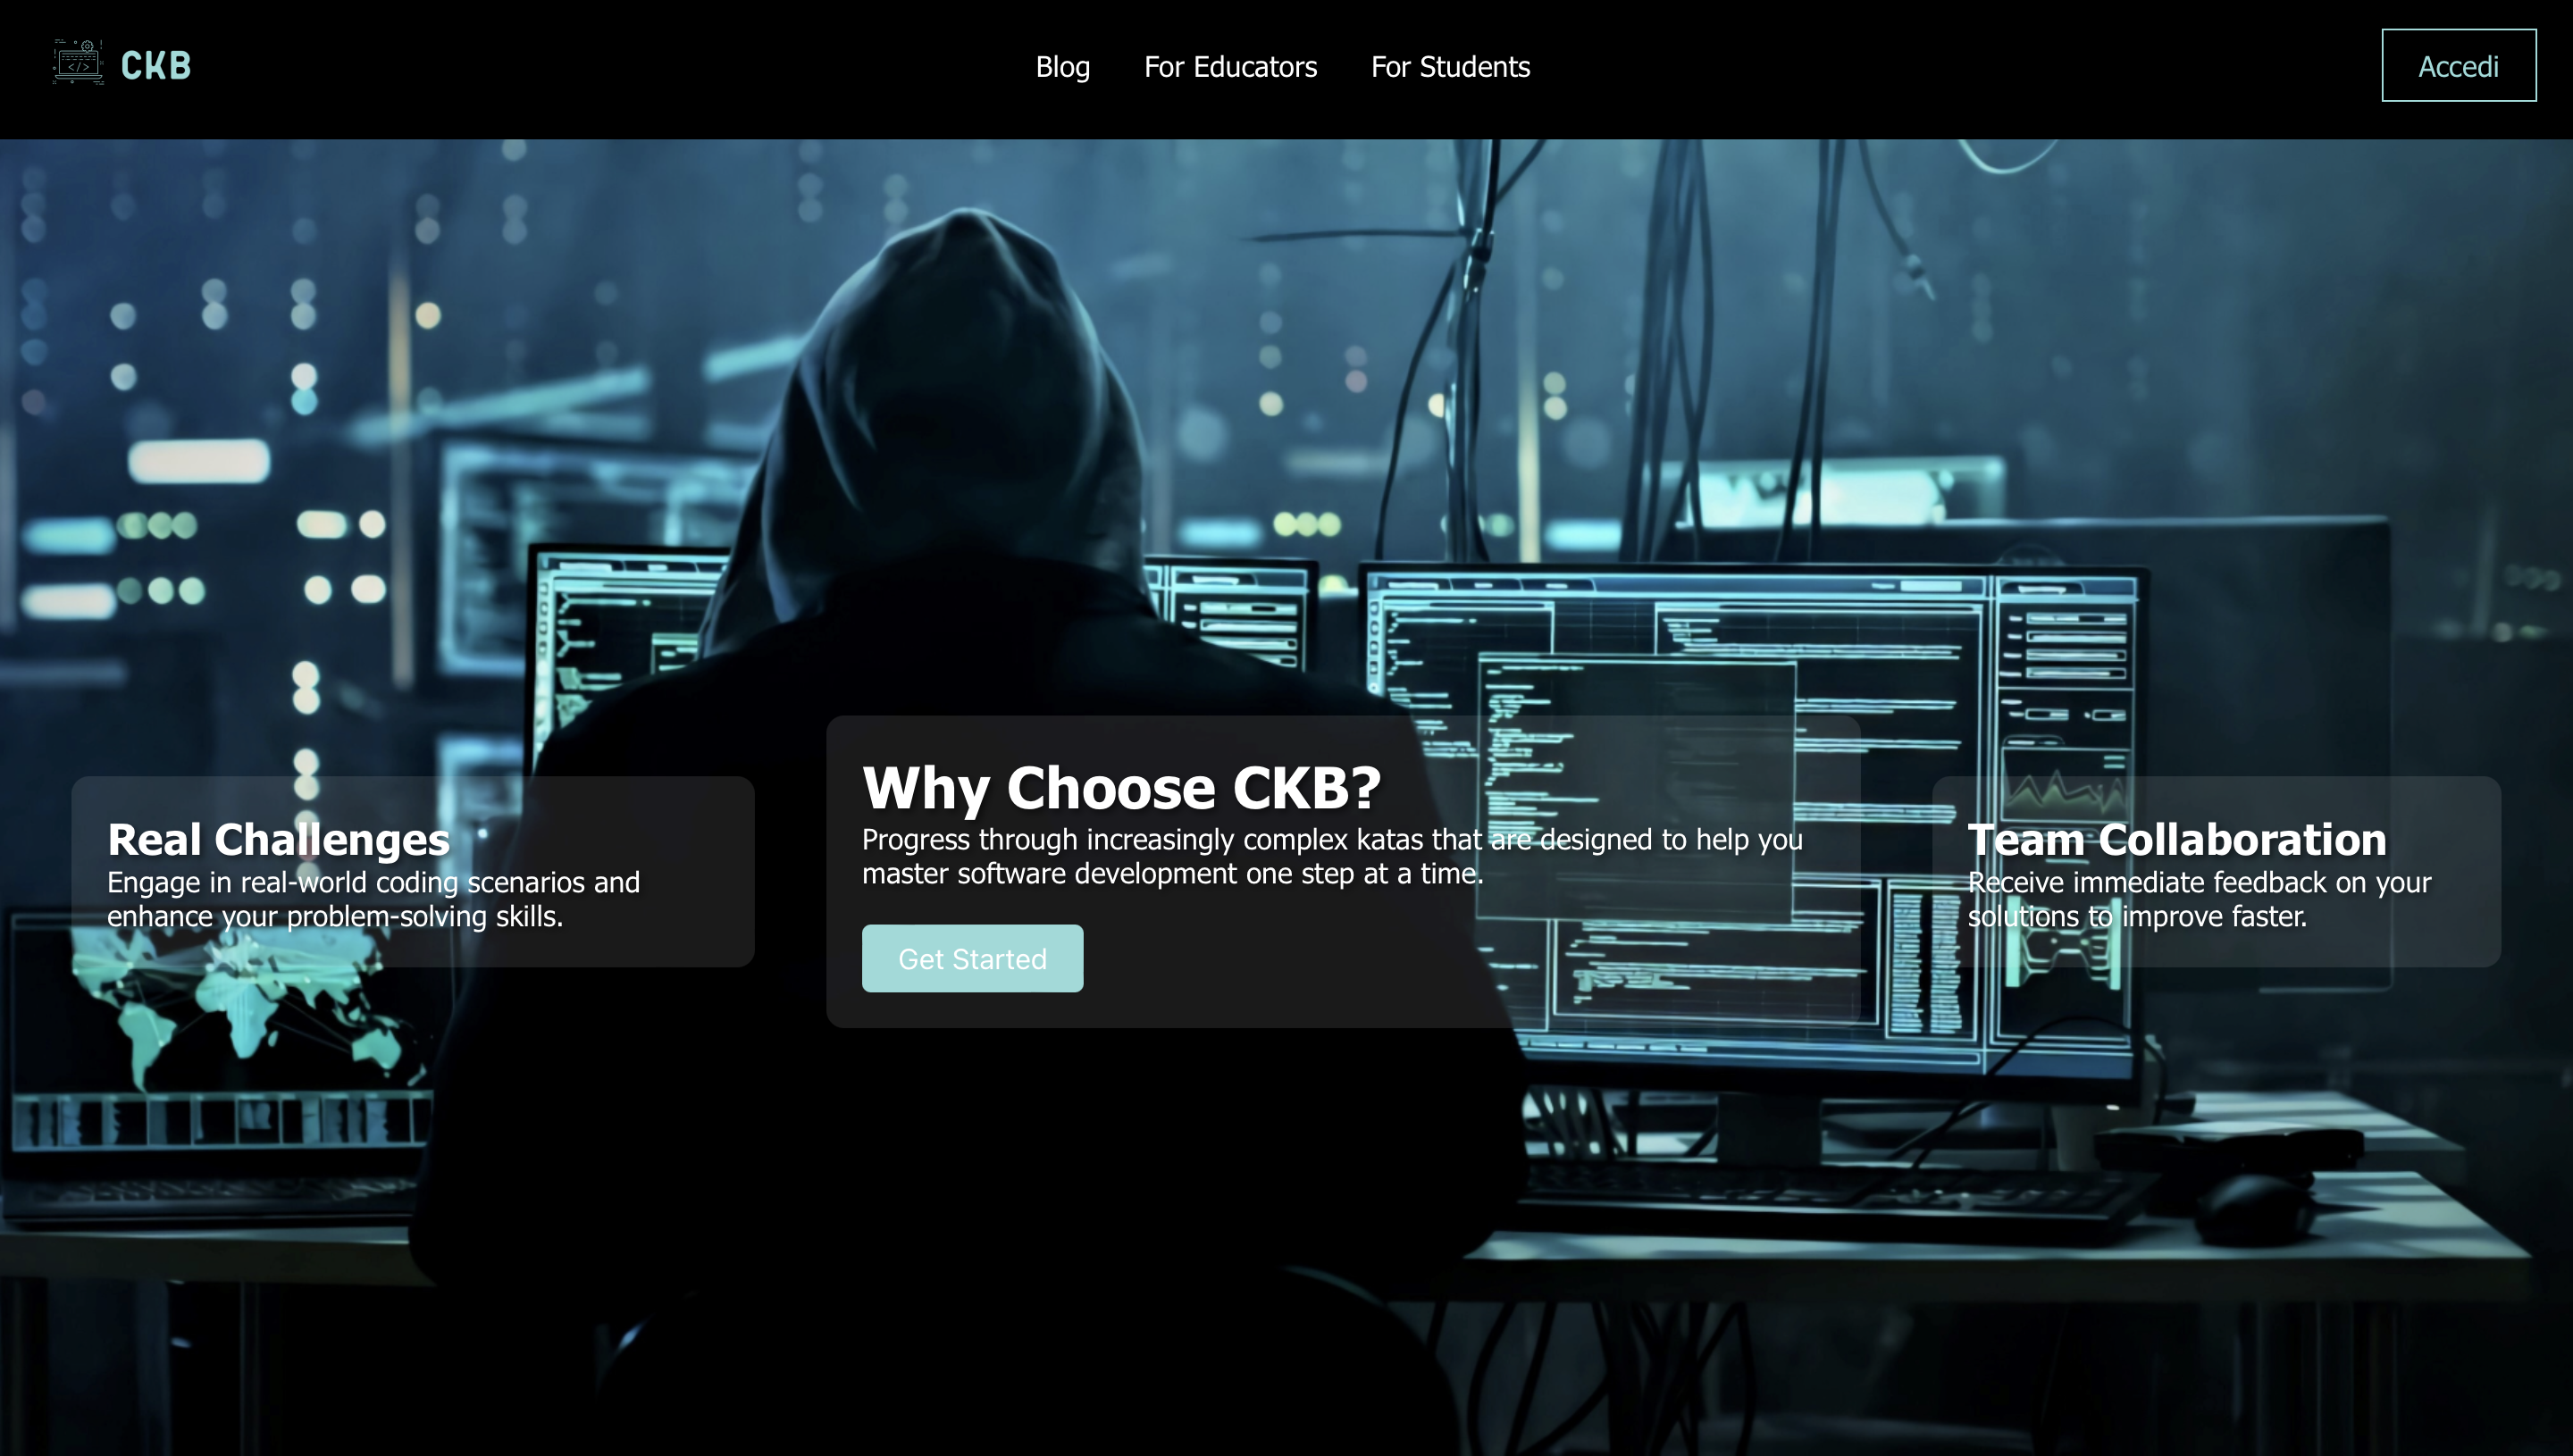
\includegraphics[width=1\linewidth]{Mockup/home.png} 
  \caption{Home Page}
  \label{fig:immagine}
\end{figure}
\\
 \begin{figure}[H]
  %\centering
  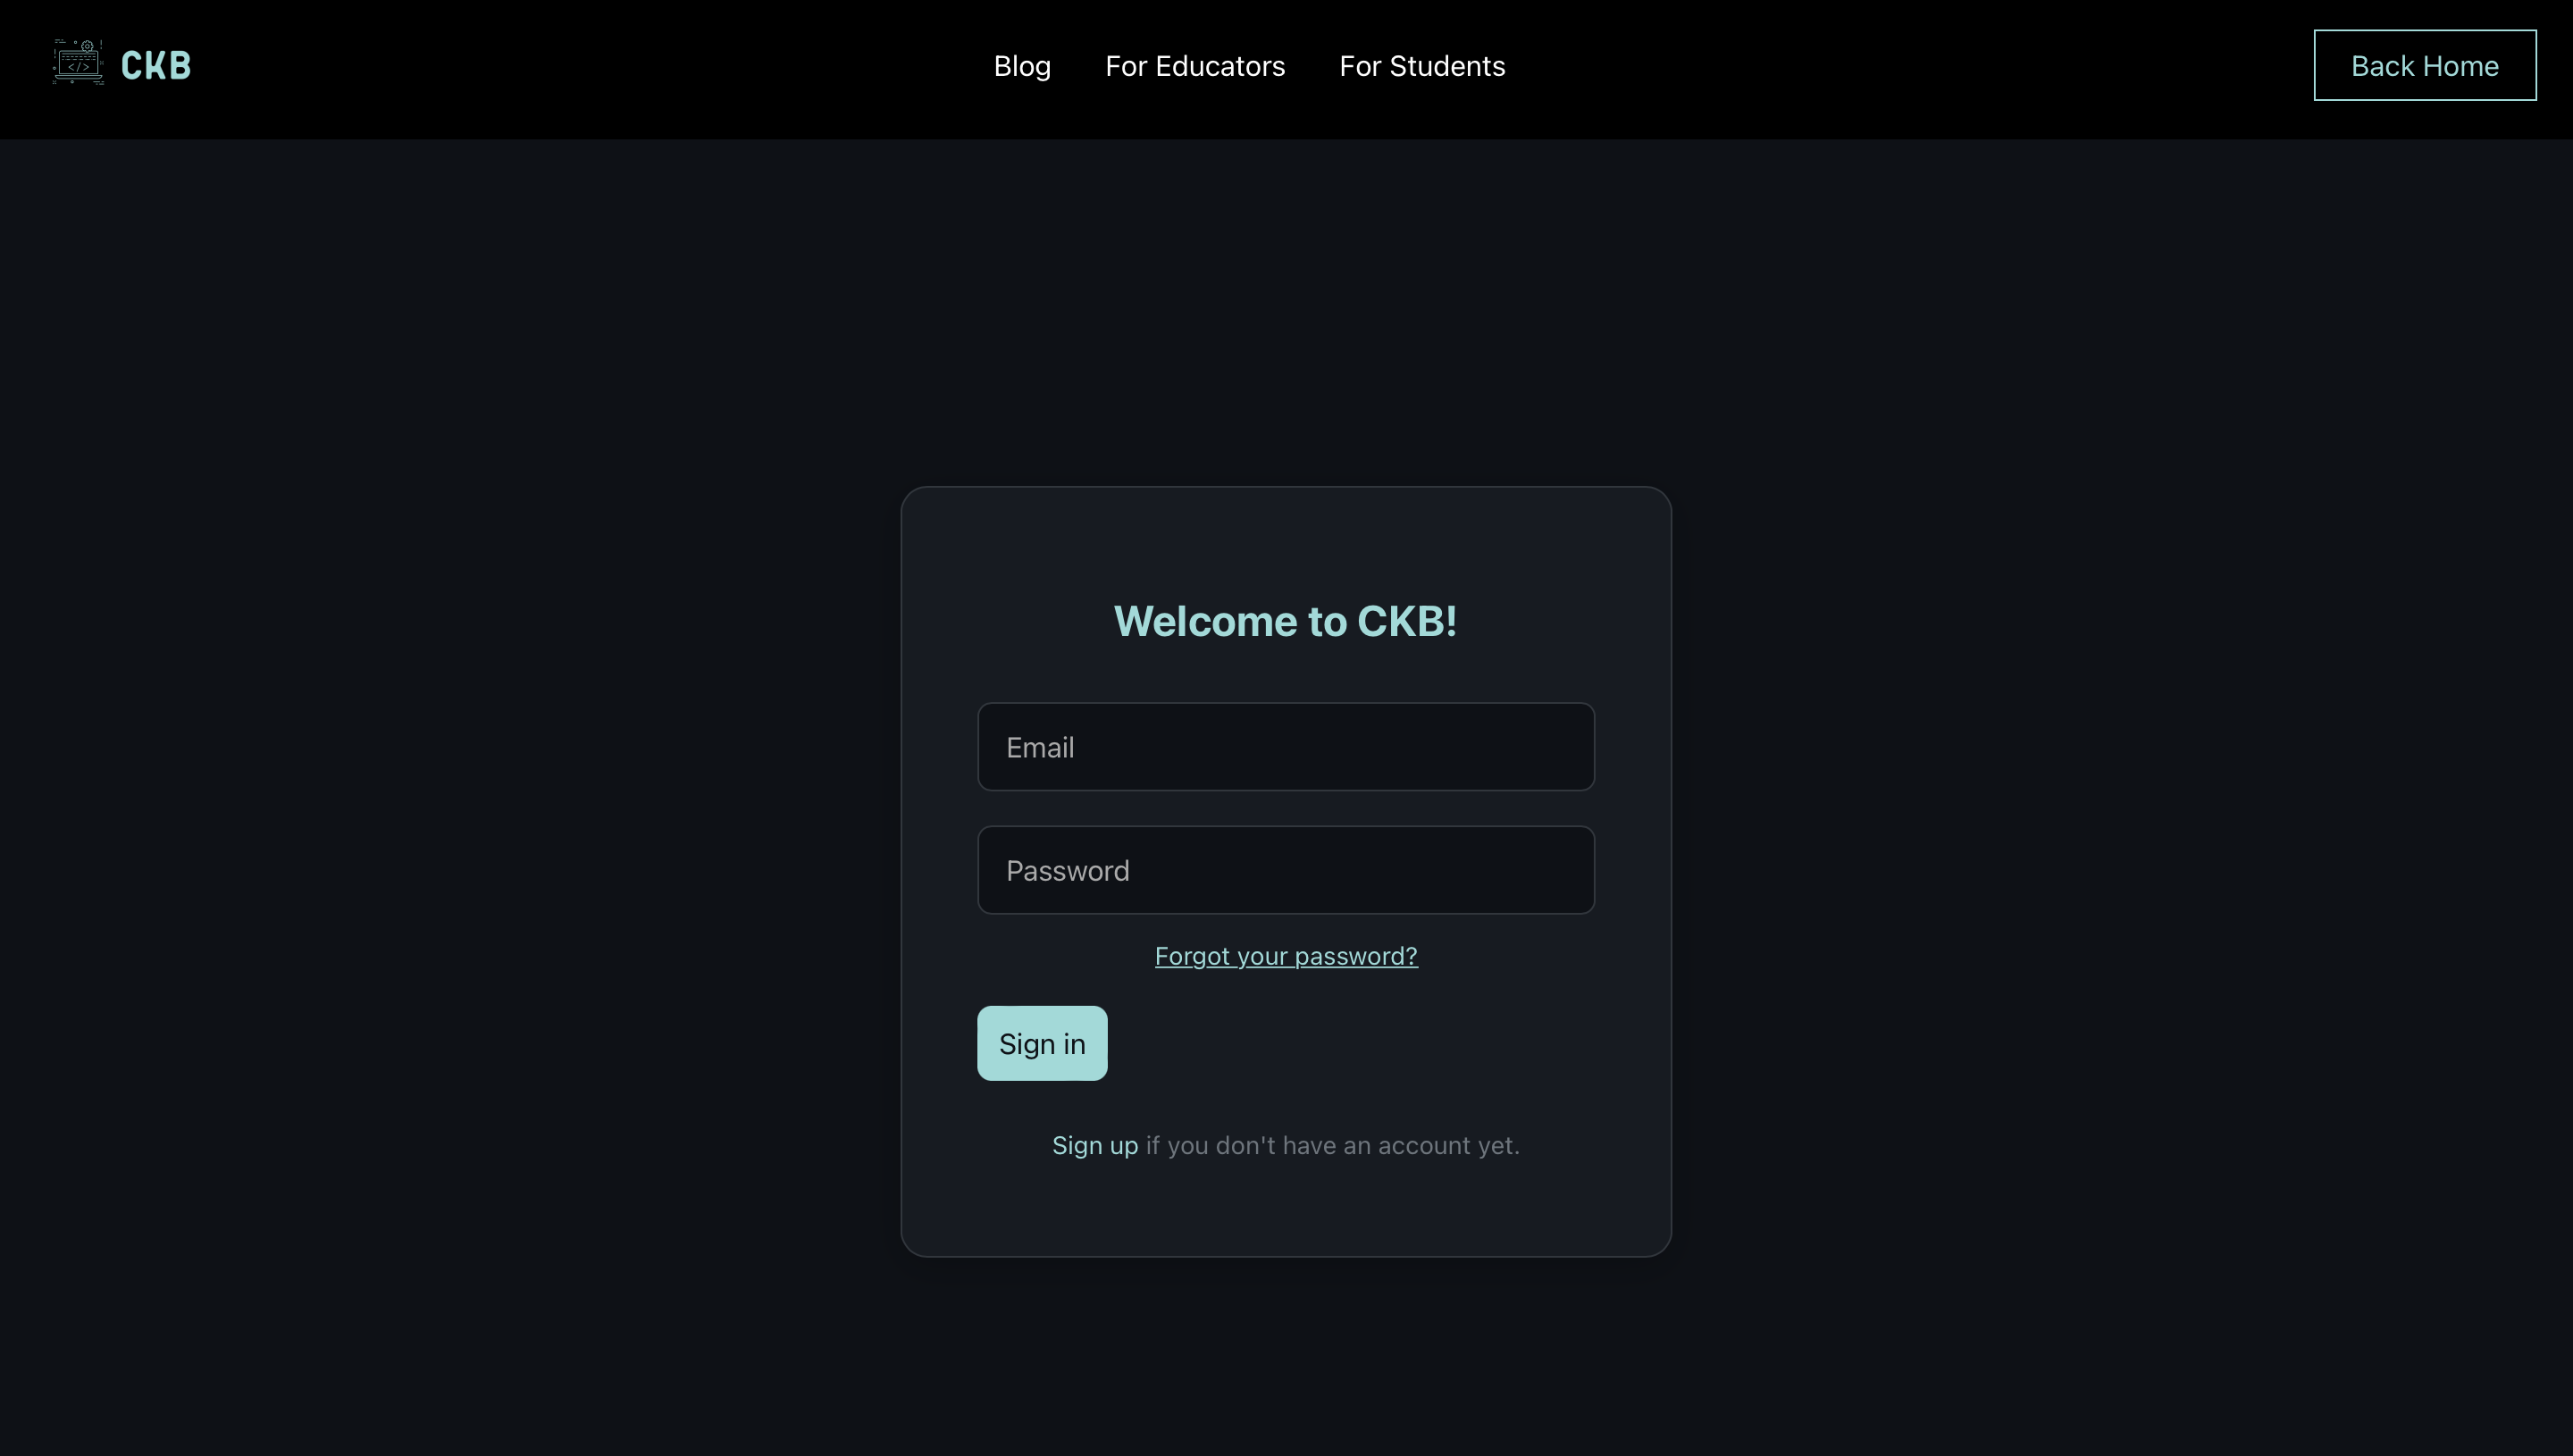
\includegraphics[width=1\linewidth]{Mockup/login.png} 
  \caption{Login Page}
  \label{fig:immagine}
\end{figure}
\\
 \begin{figure}[H]
  %\centering
  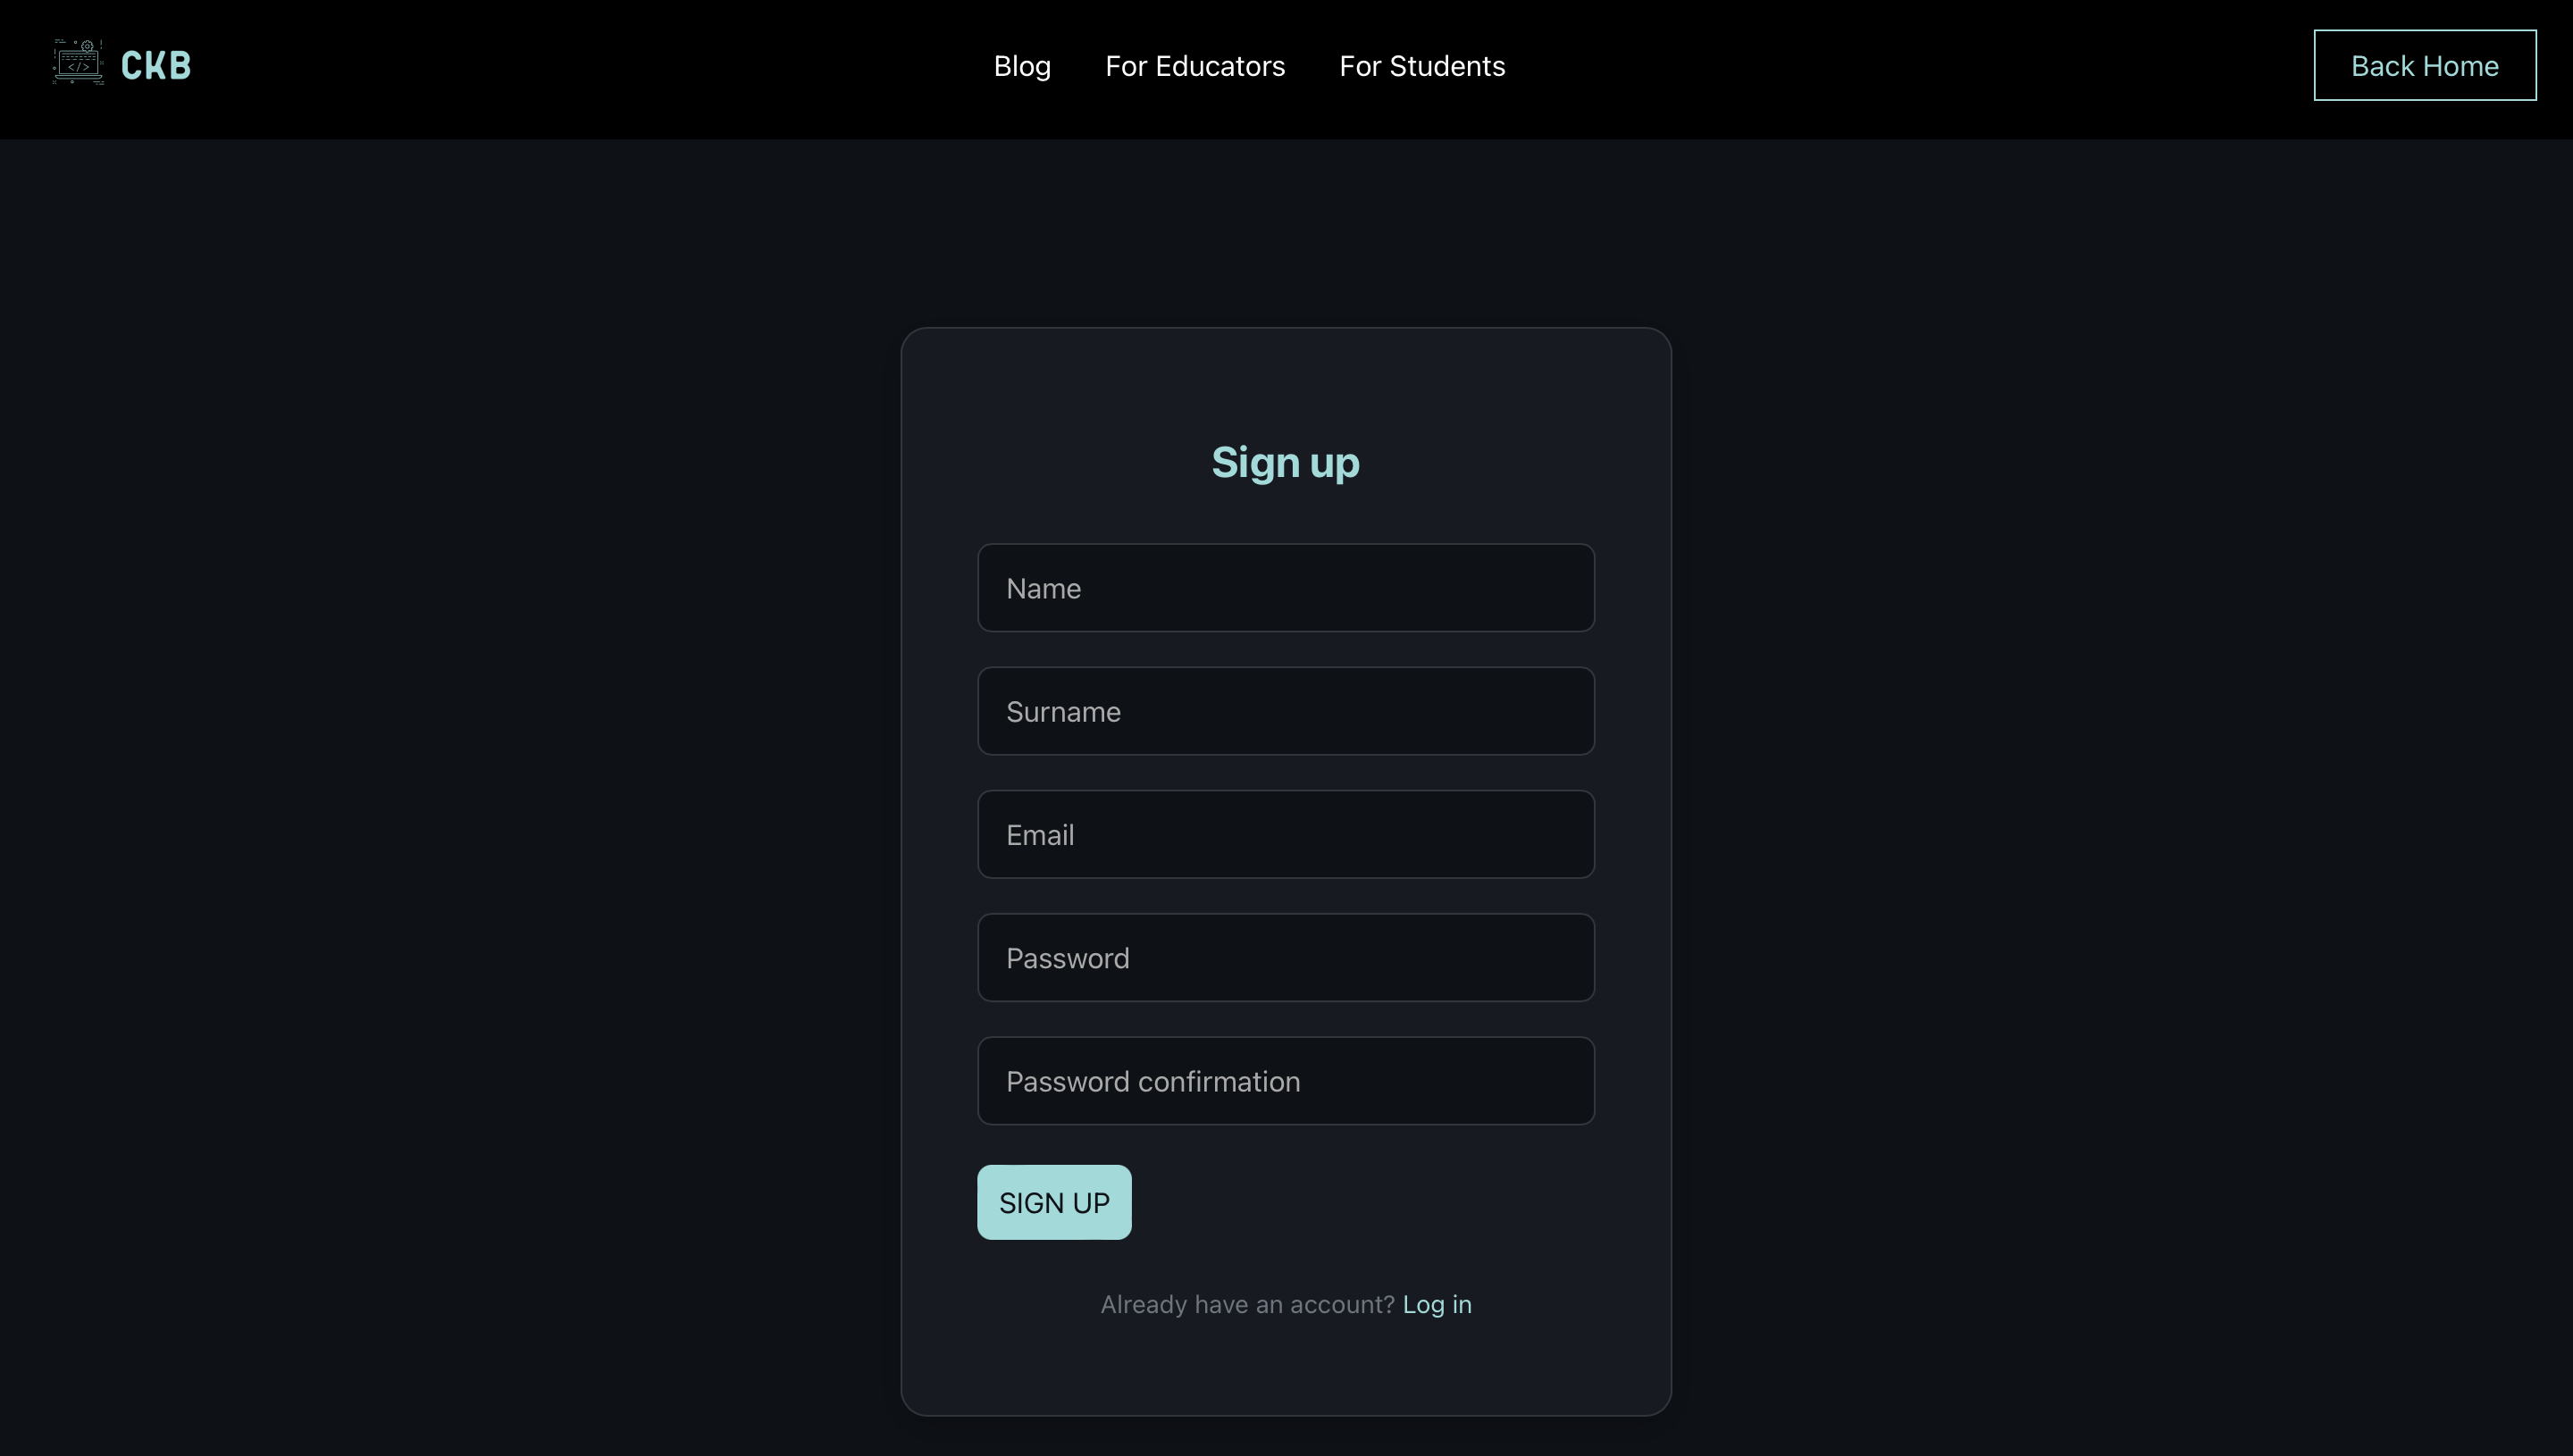
\includegraphics[width=1\linewidth]{Mockup/reg.png} 
  \caption{Registration Page}
  \label{fig:immagine}
\end{figure}


\subsection{Use case diagrams}
The following use case diagrams have been generated based on the scenarios described in paragraph 2.1.1. These diagrams assist in recognizing the individuals or entities engaging with the system and elucidate their responsibilities within each specific use case.
 \begin{figure}[H]
  %\centering
  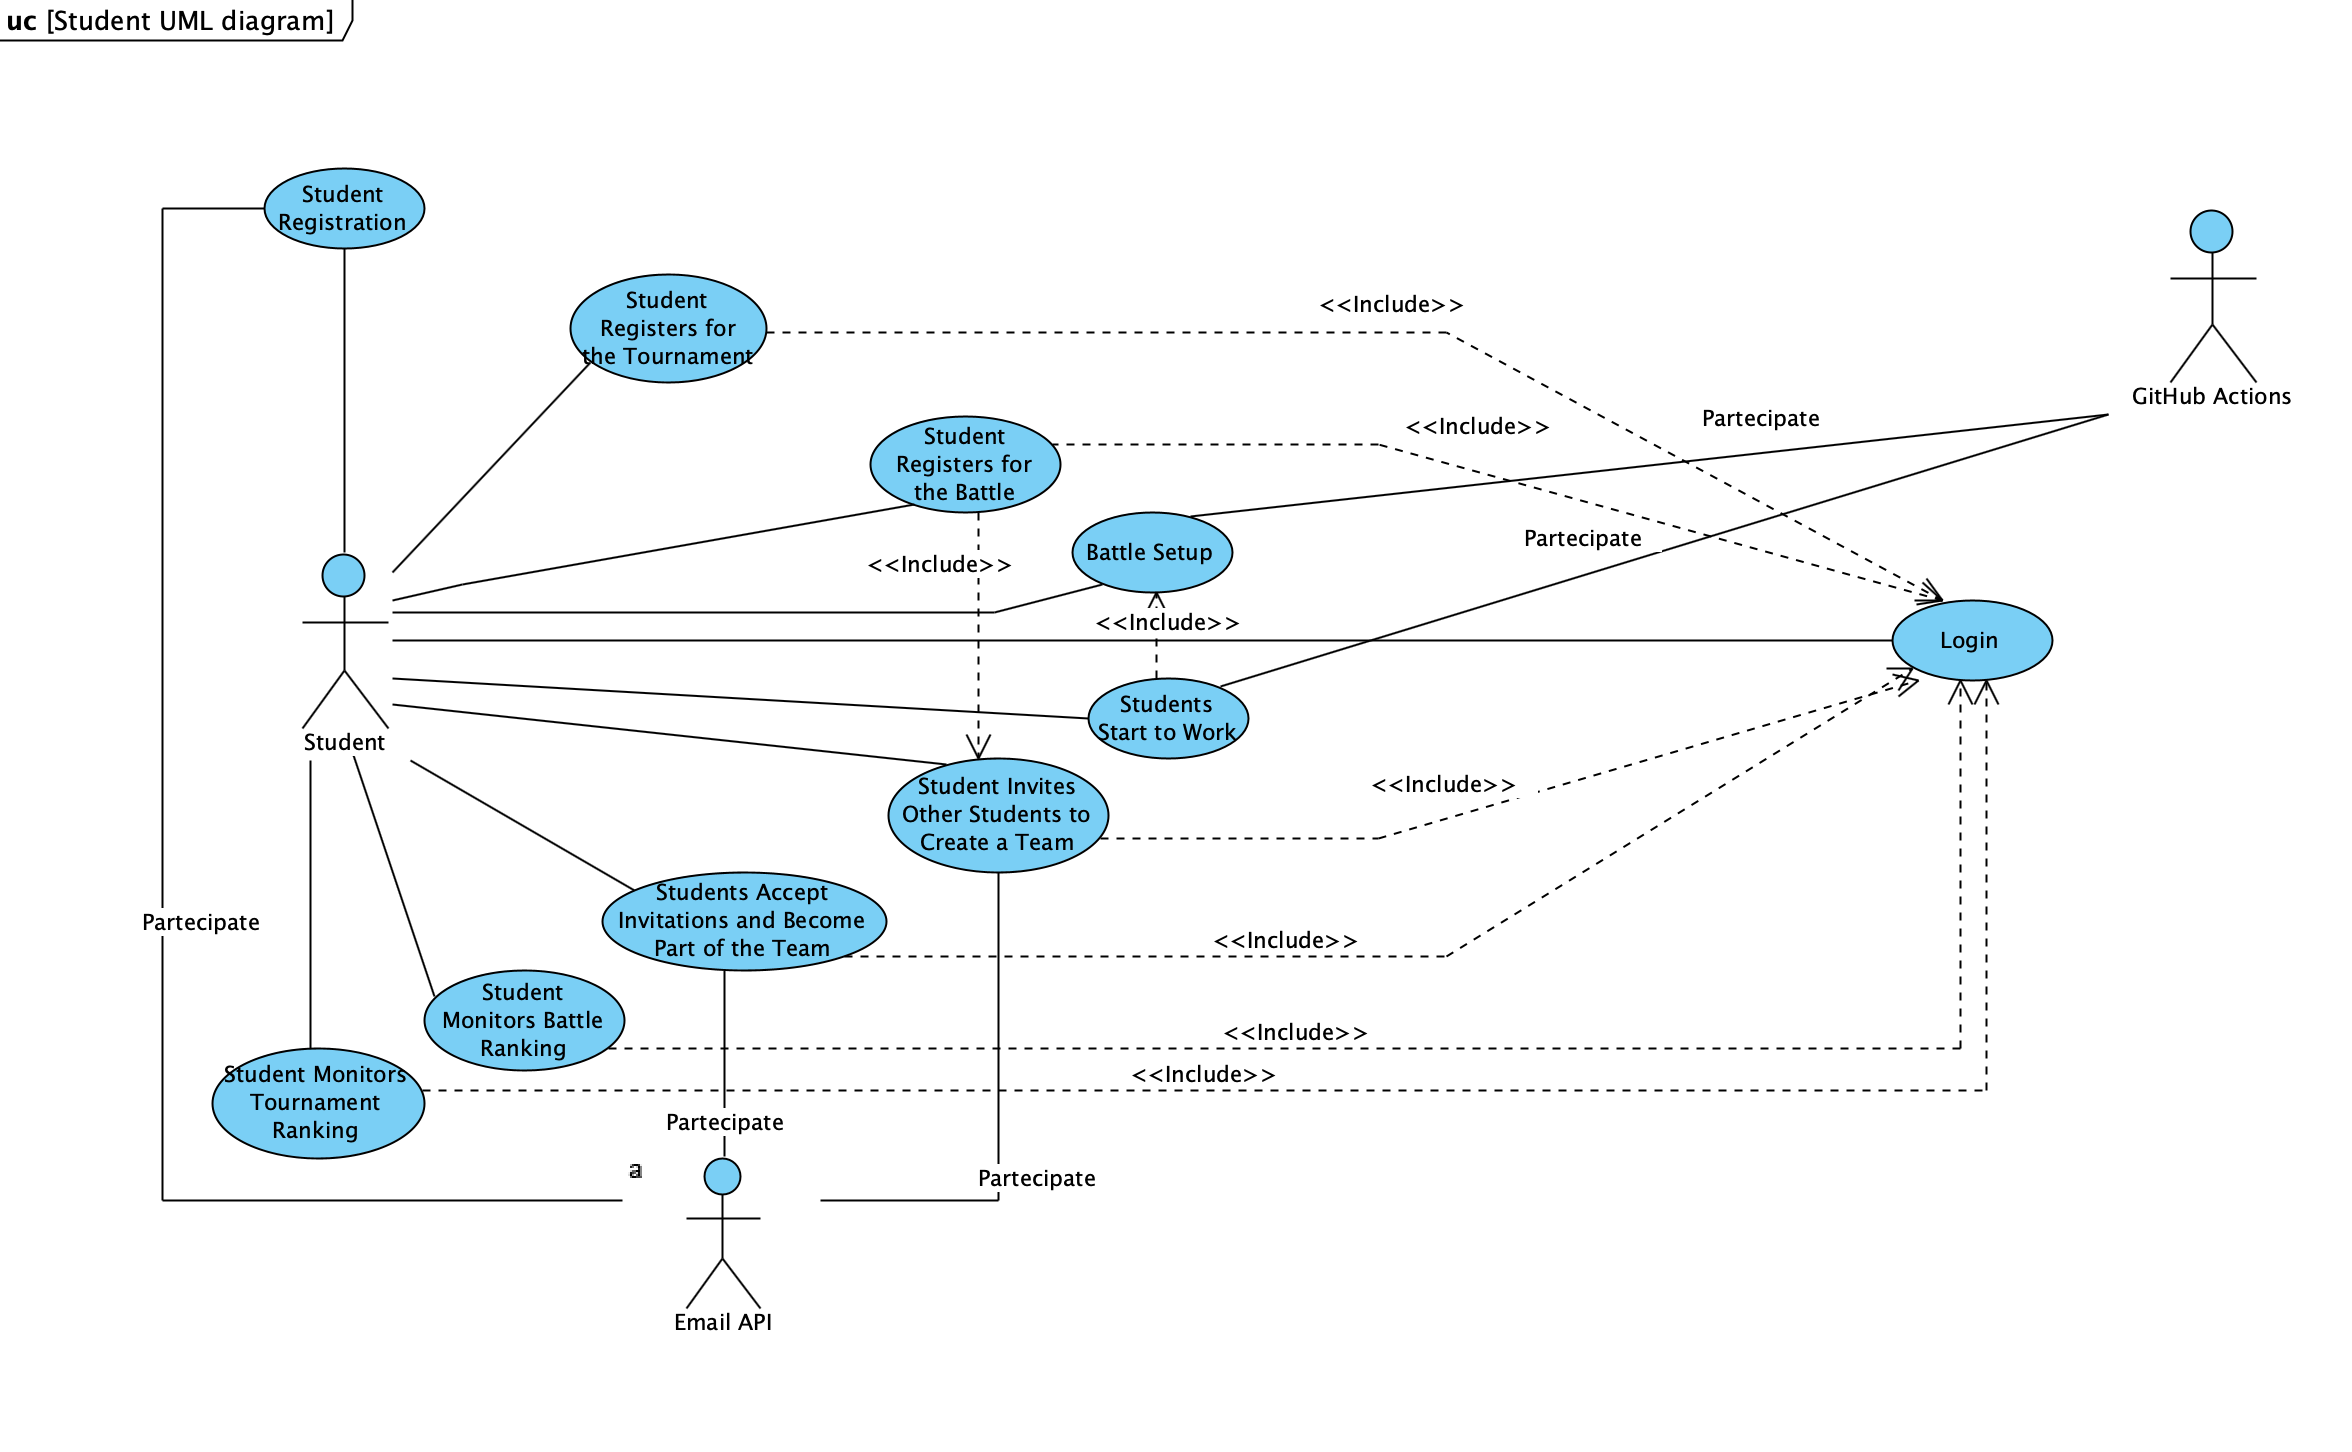
\includegraphics[width=1\linewidth]{UMLDiagram/StudentUMLDiagram.png} 
  \caption{Student use case diagram}
  \label{fig:immagine}
\end{figure}

 \begin{figure}[H]
  %\centering
  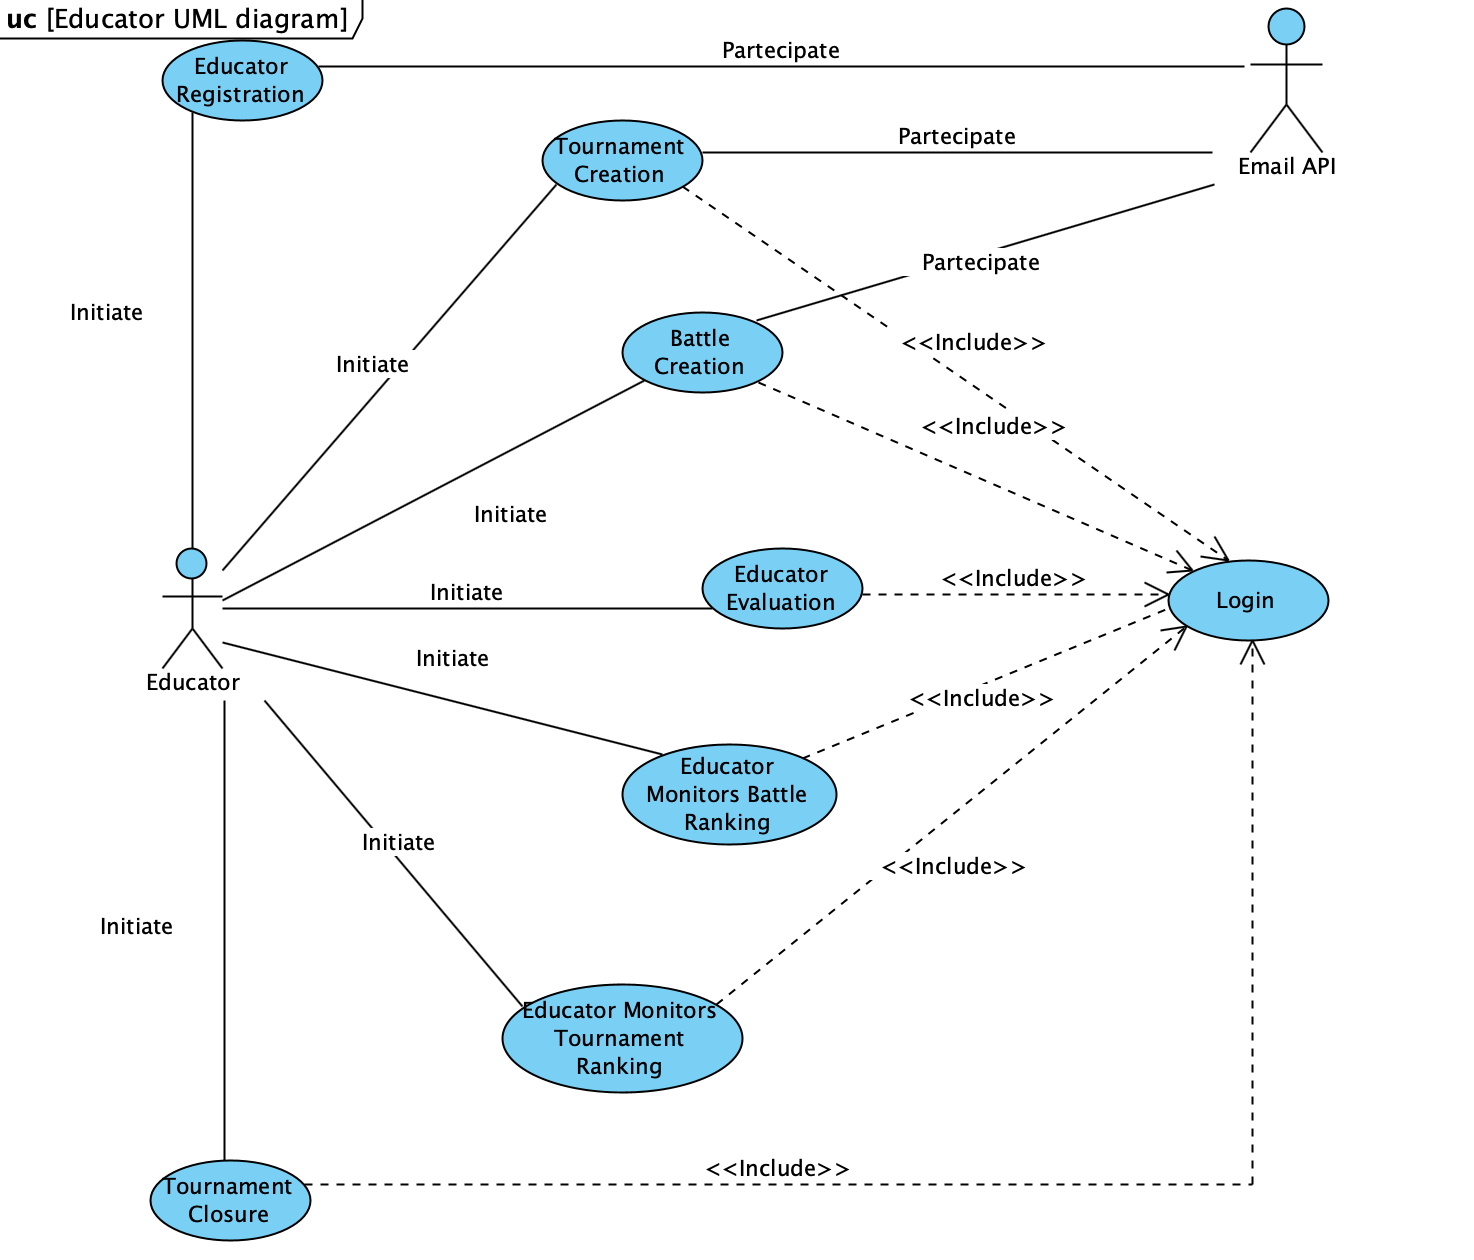
\includegraphics[width=0.8\linewidth]{UMLDiagram/EducatorUMLDiagram.png} 
  \caption{Educator use case diagram}
  \label{fig:immagine}
\end{figure}

\subsection{User's use case}
%%USE CASE EDUCATOR SI REGISTRA
\subsubsection{Educator registration}
\begin{longtable}{|c| p{10cm}|}
\hline
ID & 1 \\
\hline
Name & Educator Registration \\
\hline
Actor & Educator, email API \\
\hline
Entry Conditions &
The educator has opened the web page on his computer\\
\hline
Events Flow & \begin{enumerate}
\item On the homepage, the educator clicks on the "Register/Login" section
\item The system shows two options:
\begin{itemize}
\item Register
\item Login
\end{itemize}
\item Educator selects “Registration”
\item The system shows a list of fields that the educator needs to enter:
\begin{itemize}
\item Name
\item Surname
\item Email
\item Password
\item A checkbox to select only if you are an educator
\end{itemize}
\item Educator enters the data, selects the checkbox and accepts the "Terms of Service"
\item Educator clicks on the "Confirm" button
\item The system shows the acceptance of the registration and invites the educator to go to his mailbox to confirm the registration
\item The educator opens his mailbox, searches for the email sent by the platform and clicks on the "accept registration" link
\end{enumerate} \\
\hline
Exit Conditions &
\begin{itemize}
\item Registration successfully completed: now the educator's data has been entered into the database.
\item The educator clicks on "You already have an account: is redirected to the Login section"
\end{itemize}\\
\hline
Exceptions &
\begin{itemize}
\item The educator enters an email that is already present in the database. So, after the user clicks on the "Confirm" button, the platform shows the same page with an error message inviting the user to change the email since it is already stored in the database
\item Educator enters an incorrect email. So, after the user clicks on the "Confirm" button, the platform shows the same page with an error message inviting the user to modify the email since it is incorrect.
\item The educator does not receive the registration confirmation message in his mailbox. So, he clicks on "Send a new verification email" and the system sends a new registration confirmation link to the educator's email.
\end{itemize}\\
\hline
\end{longtable}

    \begin{figure}[H]
  %\centering
  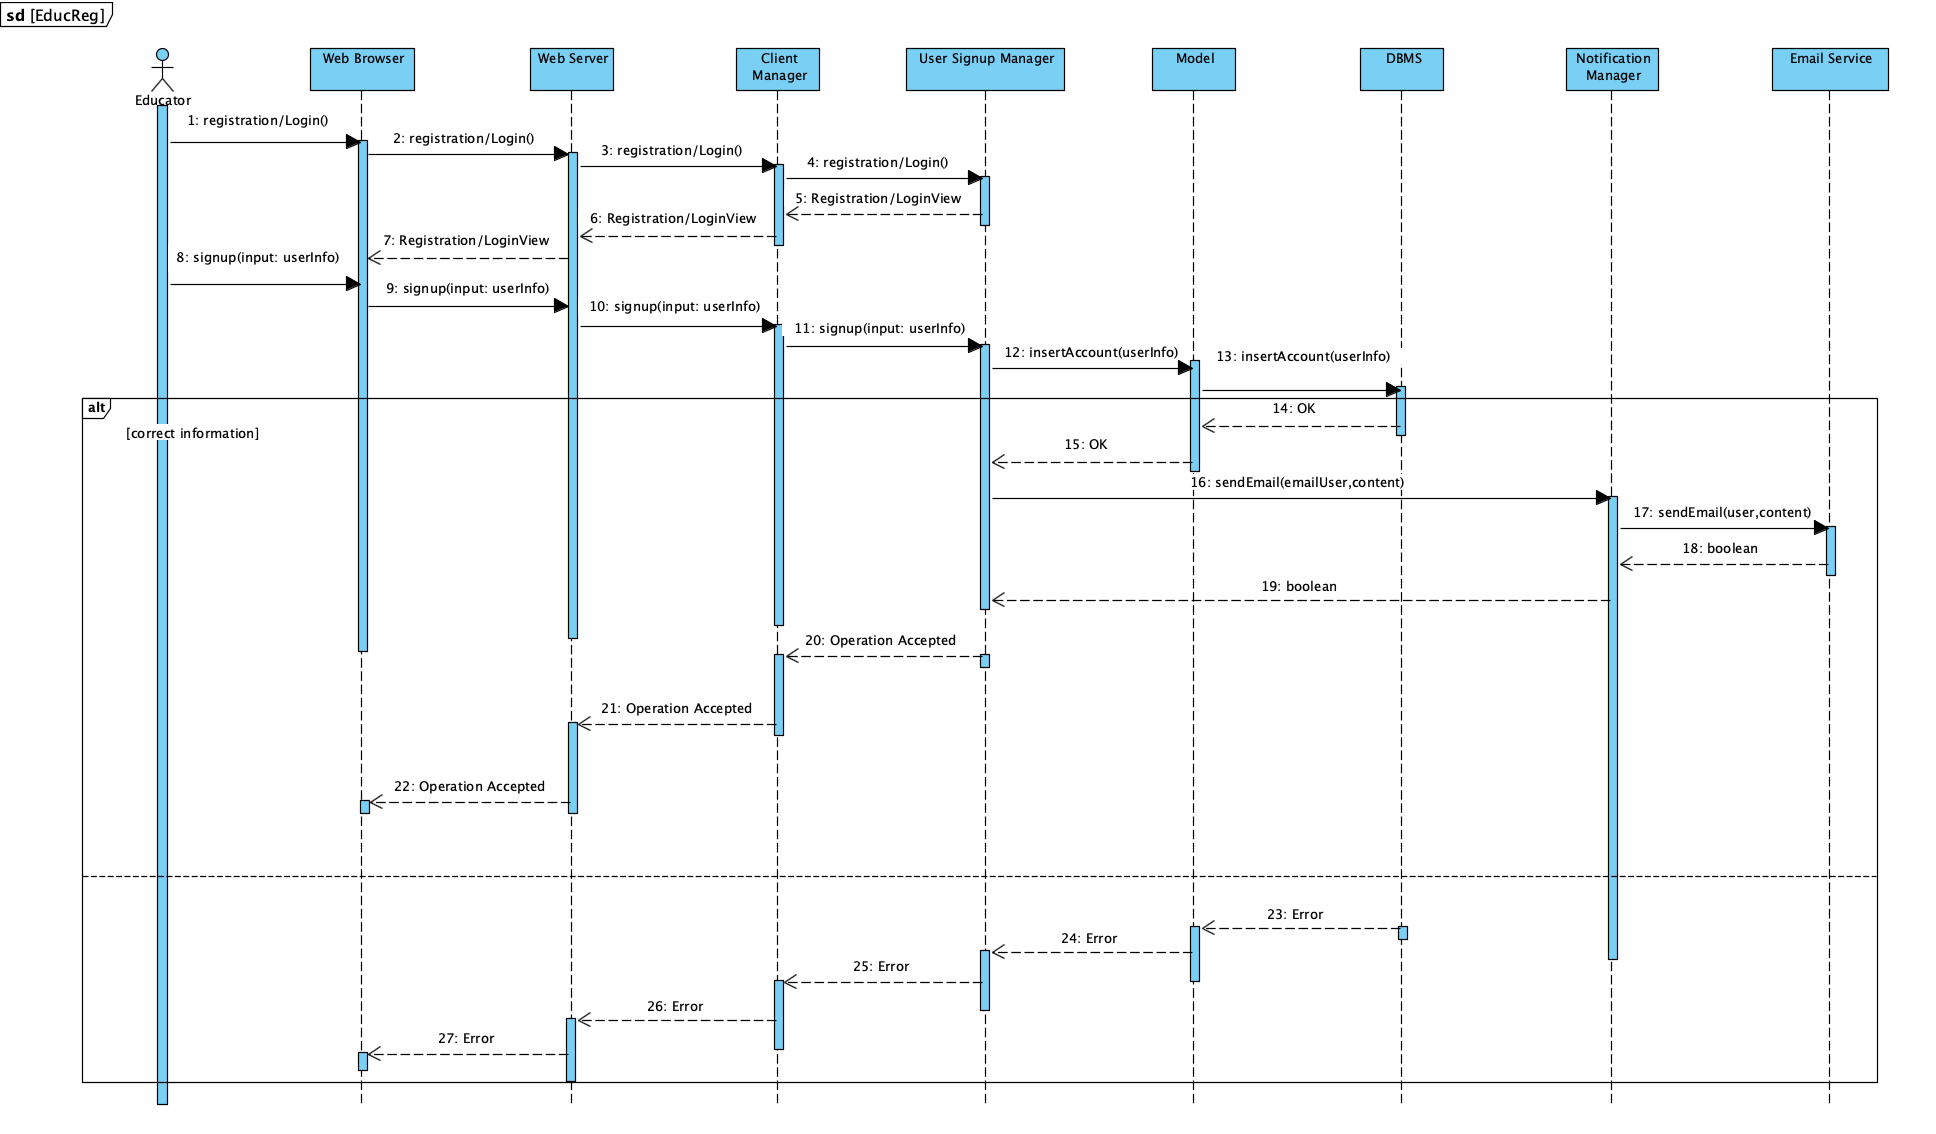
\includegraphics[width=1\linewidth]{SequenceDiagram/EducatorReg.png} 
  \caption{Educator registration}
  \label{fig:immagine}
\end{figure}



\subsubsection{Student registration}
\begin{longtable}{|c| p{10cm}|}
\hline
ID & 2 \\
\hline
Name & Student Registration \\
\hline
Actor & Student, email API \\
\hline
Entry Conditions &
The student has opened the web page on his computer\\
\hline
Events Flow & \begin{itemize}
\item On the homepage, the student clicks on the "Register/Login" section
\item The system shows two options:
\begin{itemize}
\item Register
\item Login
\end{itemize}
\item Student selects “Registration”
\item The system shows a list of fields that the student needs to enter:
\begin{itemize}
\item Name
\item Surname
\item Email
\item Password
\item A checkbox to select only if you are a student
\end{itemize}
\item Student enters the data,does not select the checkbox and accepts the "Terms of Service"
\item Student clicks on the "Confirm" button
\item The system shows the acceptance of the registration and invites the student to go to their mailbox to confirm the registration
\item The student opens their mailbox, searches for the email sent by the platform, and clicks on the "accept registration" link
\end{itemize} \\
\hline
Exit Conditions &
\begin{itemize}
\item Registration successfully completed: now the student's data has been entered into the database.
\item The student clicks on "You already have an account: is redirected to the Login section"
\end{itemize}\\
\hline
Exceptions &
\begin{itemize}
\item The student enters an email that is already present in the database. So, after the user clicks on the "Confirm" button, the platform shows the same page with an error message inviting the user to change the email since it is already stored in the database
\item Student enters an incorrect email. So, after the user clicks on the "Confirm" button, the platform shows the same page with an error message inviting the user to modify the email since it is incorrect.
\item The student does not receive the registration confirmation message in his mailbox. So, he clicks on "Send a new verification email", and the system sends a new registration confirmation link to the student's email.
\end{itemize}\\
\hline
\end{longtable}

    \begin{figure}[H]
  %\centering
  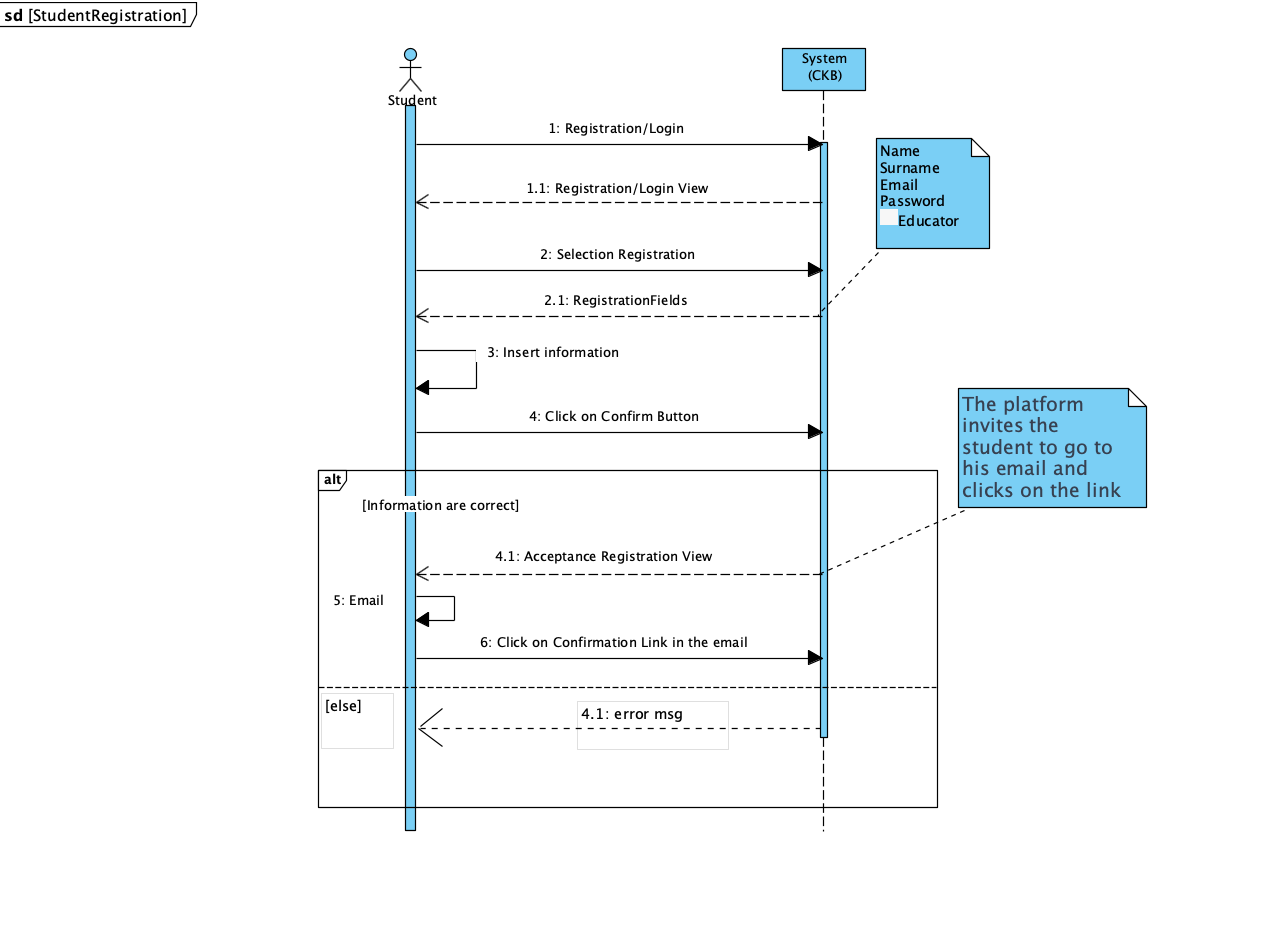
\includegraphics[width=1\linewidth]{SequenceDiagram/StudReg.png} 
  \caption{Student registration}
  \label{fig:immagine}
\end{figure}

\newpage
\subsubsection{User Login}
\begin{longtable}{|c| p{10cm}|}
\hline
ID & 3 \\
\hline
Name & User Login \\
\hline
Actor & Educator or Student \\
\hline
Entry Conditions &
The user has opened the web page on his computer
\\
\hline
Events Flow &
\begin{enumerate}
\item On the homepage, the user clicks on the "Register/Login" section.
\item The system shows two options:
\begin{itemize}
\item Register
\item Login
\end{itemize}
\item User selects Login.
\item The system shows a list of fields that the user needs to enter:
\begin{itemize}
\item Email
\item Password
\end{itemize}
\item The user clicks the "Confirm" button.
\item The system verifies the credentials.
\end{enumerate} \\
\hline
Exit Conditions &
\begin{itemize}
\item Login is successfully completed, and the platform displays the user's profile dashboard.
\end{itemize}\\
\hline
Exceptions &
\begin{itemize}
\item The user enters incorrect credentials. So, after the user clicks the "Confirm" button, the platform displays the same page with an error message explaining that the credentials are incorrect.
\item If the user makes too many login attempts, the platform redirects them to the initial homepage with an error message specifying that they have made too many attempts and blocks the login for 30 minutes.
\end{itemize} \\
\hline
\end{longtable}

    \begin{figure}[H]
  %\centering
  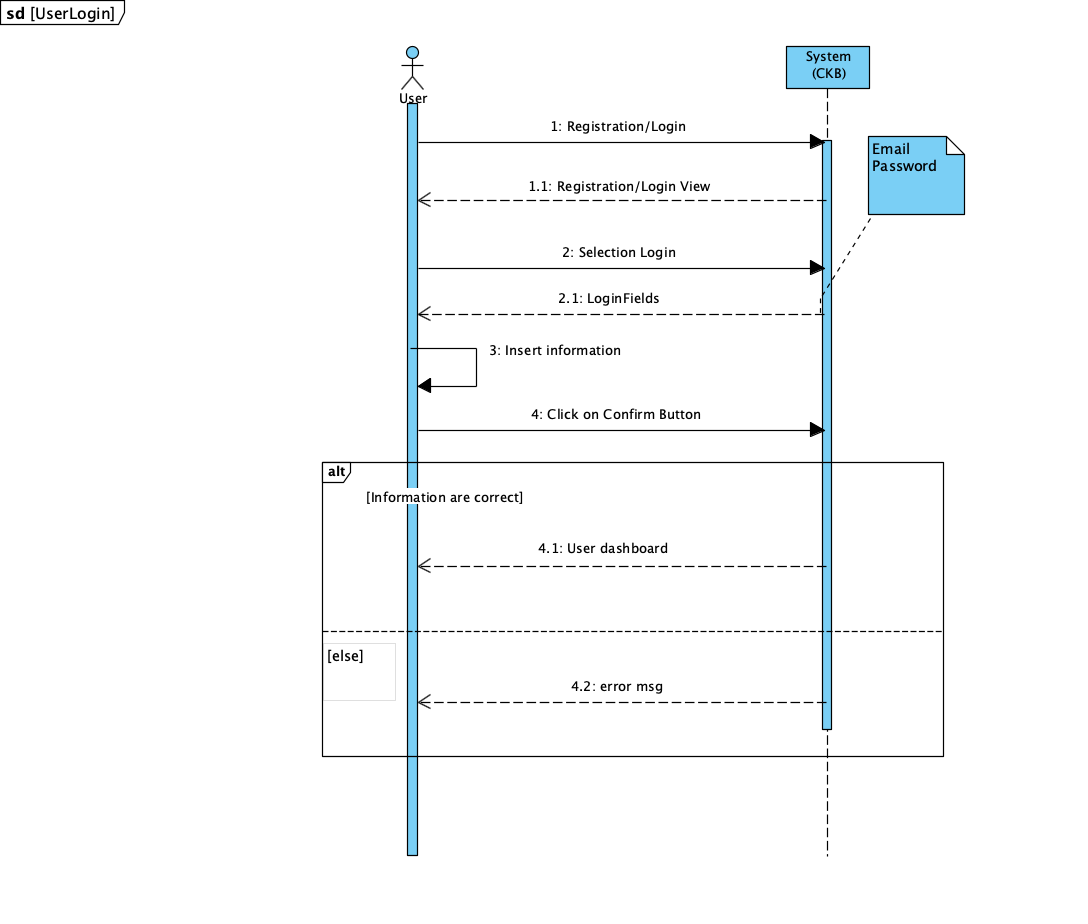
\includegraphics[width=1\linewidth]{SequenceDiagram/UserLogin.png} 
  \caption{User Login}
  \label{fig:immagine}
\end{figure}

%% TOURNAMENT CREATION
\subsubsection{Tournament creation}

\begin{longtable}{|c| p{10cm}|}
        \hline
            ID & 4 \\
        \hline
            Name & Tournament creation \\
        \hline
            Actor & Educator, email API \\
        \hline
            Entry Conditions & 
                                The educator has logged into the system.
                                \\
        \hline
            Events Flow &   \begin{enumerate}
                                \item The educator, through the homepage, clicks on the "Tournament" section.
                                \item The system presents a control dashboard that displays the tournaments created by the educator or those for which they have permission to organize battles.
                                \item The educator clicks on "Create tournament."
                                \item The system shows a list of fields that the educator needs to enter:
                                \begin{itemize}
                                    \item Tournament name
                                    \item Tournament description
                                    \item Registration Deadline
                                    \item List of email addresses of educators who have permission to create battles within the tournament
                                \end{itemize}
                                \item The educator fills in the various fields and clicks the "Confirm" button.
                                \item The system checks that the email addresses entered by the educator are valid and exist in the database.
                                \item The tournament creation is successfully completed: the platform stores the tournament information in the database and displays the following message to the user: "Tournament created successfully."
                            \end{enumerate} \\
                            \hline
            Exit Conditions &
            \begin{itemize}
                                    \item The tournament is added to the educator's tournaments section dashboard.
                                    \item The system notified via email all students subscribed to the platform.
                                \end{itemize}\\
        \hline
            Exceptions & \begin{itemize}
                \item The tournament name entered by the educator is already assigned to another tournament. Therefore, once the educator clicks the "Confirm" button, the platform displays the same page with an error message instructing the educator to change the name as it already exists.
                \item One of the email addresses entered by the educator is incorrect. Therefore, the system displays the same page to the educator but with an error message explaining that at least one of the entered emails is incorrect.
                \item One of the email addresses entered by the educator is not present in the database. Therefore, the system displays the same page to the educator but with an error message explaining that at least one of the educators is not registered on the platform.
            \end{itemize} \\
        \hline
    \end{longtable}

    \begin{figure}[H]
  %\centering
  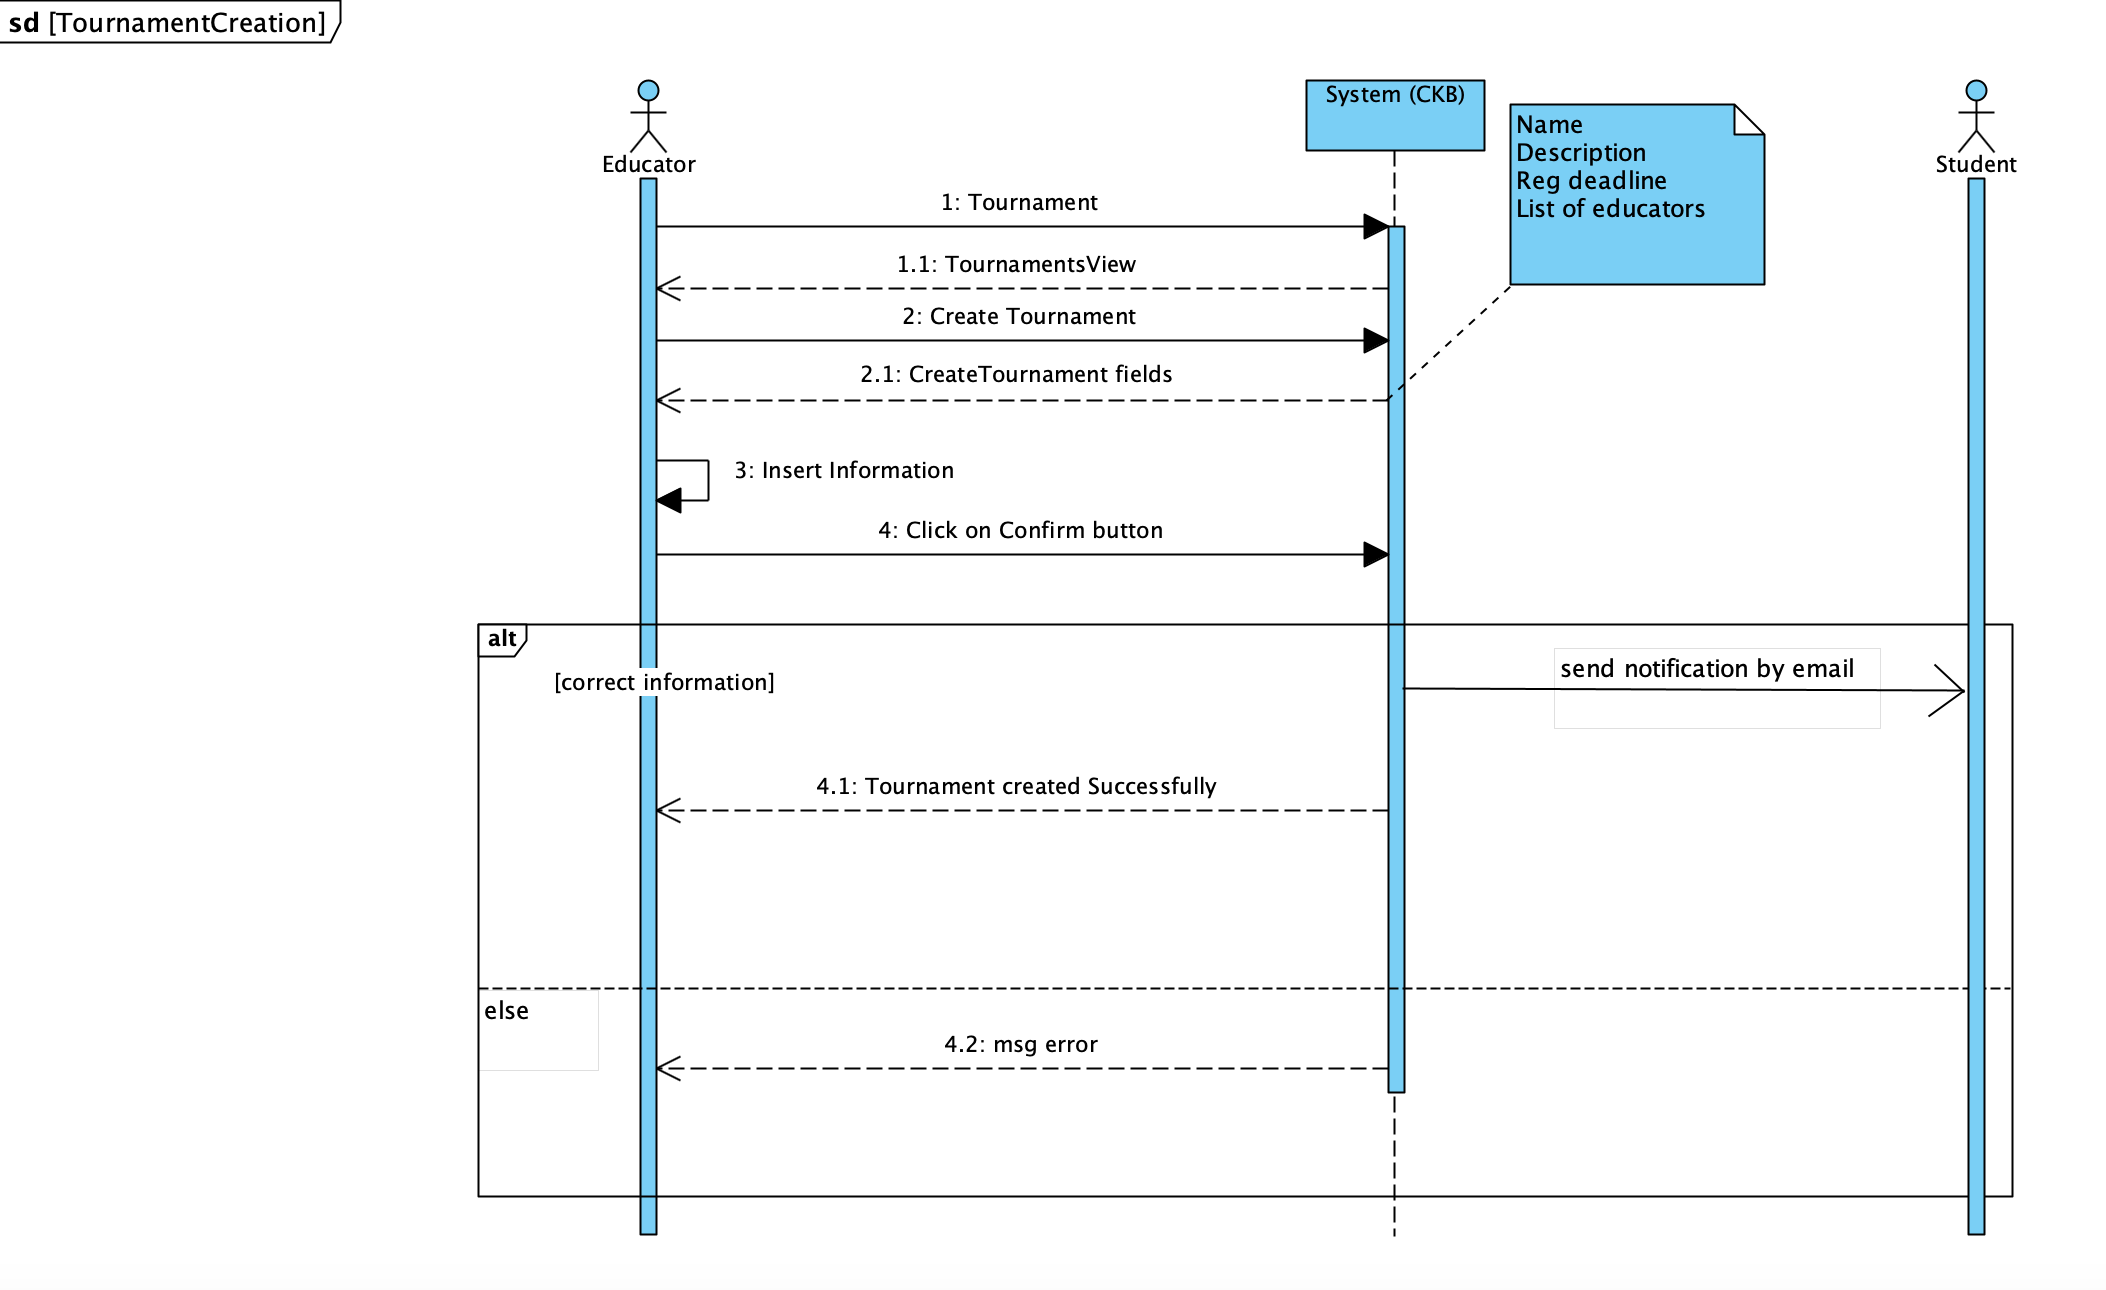
\includegraphics[width=1\linewidth]{SequenceDiagram/TournamentCreation.png} 
  \caption{Tournament creation}
  \label{fig:immagine}
\end{figure}
%% BATTLE CREATION
\subsubsection{Battle creation}

\begin{longtable}{|c| p{10cm}|}
    \hline
        ID & 5 \\
    \hline
        Name & Battle creation \\
    \hline
        Actor & Educator, email API \\
    \hline
        Entry Conditions & 
            
            The educator has logged into the system.
            \\
    \hline
        Events Flow &   \begin{enumerate}
                            \item The educator, through the homepage, clicks on the "Tournament" section.
                            \item The system presents a control dashboard that displays the tournaments created by the educator or those for which they have permission to organize battles.
                            \item The educator clicks on a specific tournament (for which they have permission to create battles).
                            \item The system displays the dashboard containing battles for the selected tournament to the educator.
                            \item The educator clicks on "Create a new battle"
                            \item The system shows a list of fields that the educator needs to enter:
                            \begin{itemize}
                                \item Upload Code Kata
                                \item Minimum number of students to form a team
                                \item Maximum number of students to form a team
                                \item A checkbox to enable the manual evaluation of the educator on the projects
                                \item A checkbox to select only if security considerations are required in the static analysis of the project submitted by the students.
                                \item A checkbox to select only if reliability considerations are required in the static analysis of the project submitted by the students.
                                \item A checkbox to select only if maintainability considerations are required in the static analysis of the project submitted by the students.
                            \end{itemize}
                            \item The educator fills in the various fields, selects the checkboxes of interest and clicks the "Confirm" button.
                            \item The system checks that the battle name is not already in use.
                            \item The battle creation is successfully completed: the platform stores the battle information in the database and displays the following message to the user: "Battle created successfully."
                        \end{enumerate} \\
    \hline
        Exit Conditions &
        \begin{itemize}
            \item The battle is added to the dashboard of the specific tournament.
            \item All students registered for the specific tournament selected by the educator are notified of the battle creation via email.
        \end{itemize}\\
    \hline
        Exceptions & 
            The battle name entered by the educator is already assigned to another battle in the same tournament. Therefore, when the educator clicks the "Confirm" button, the platform displays the same page with an error message instructing the educator to change the name as it already exists.
        \\
    \hline
\end{longtable}

    \begin{figure}[H]
  %\centering
  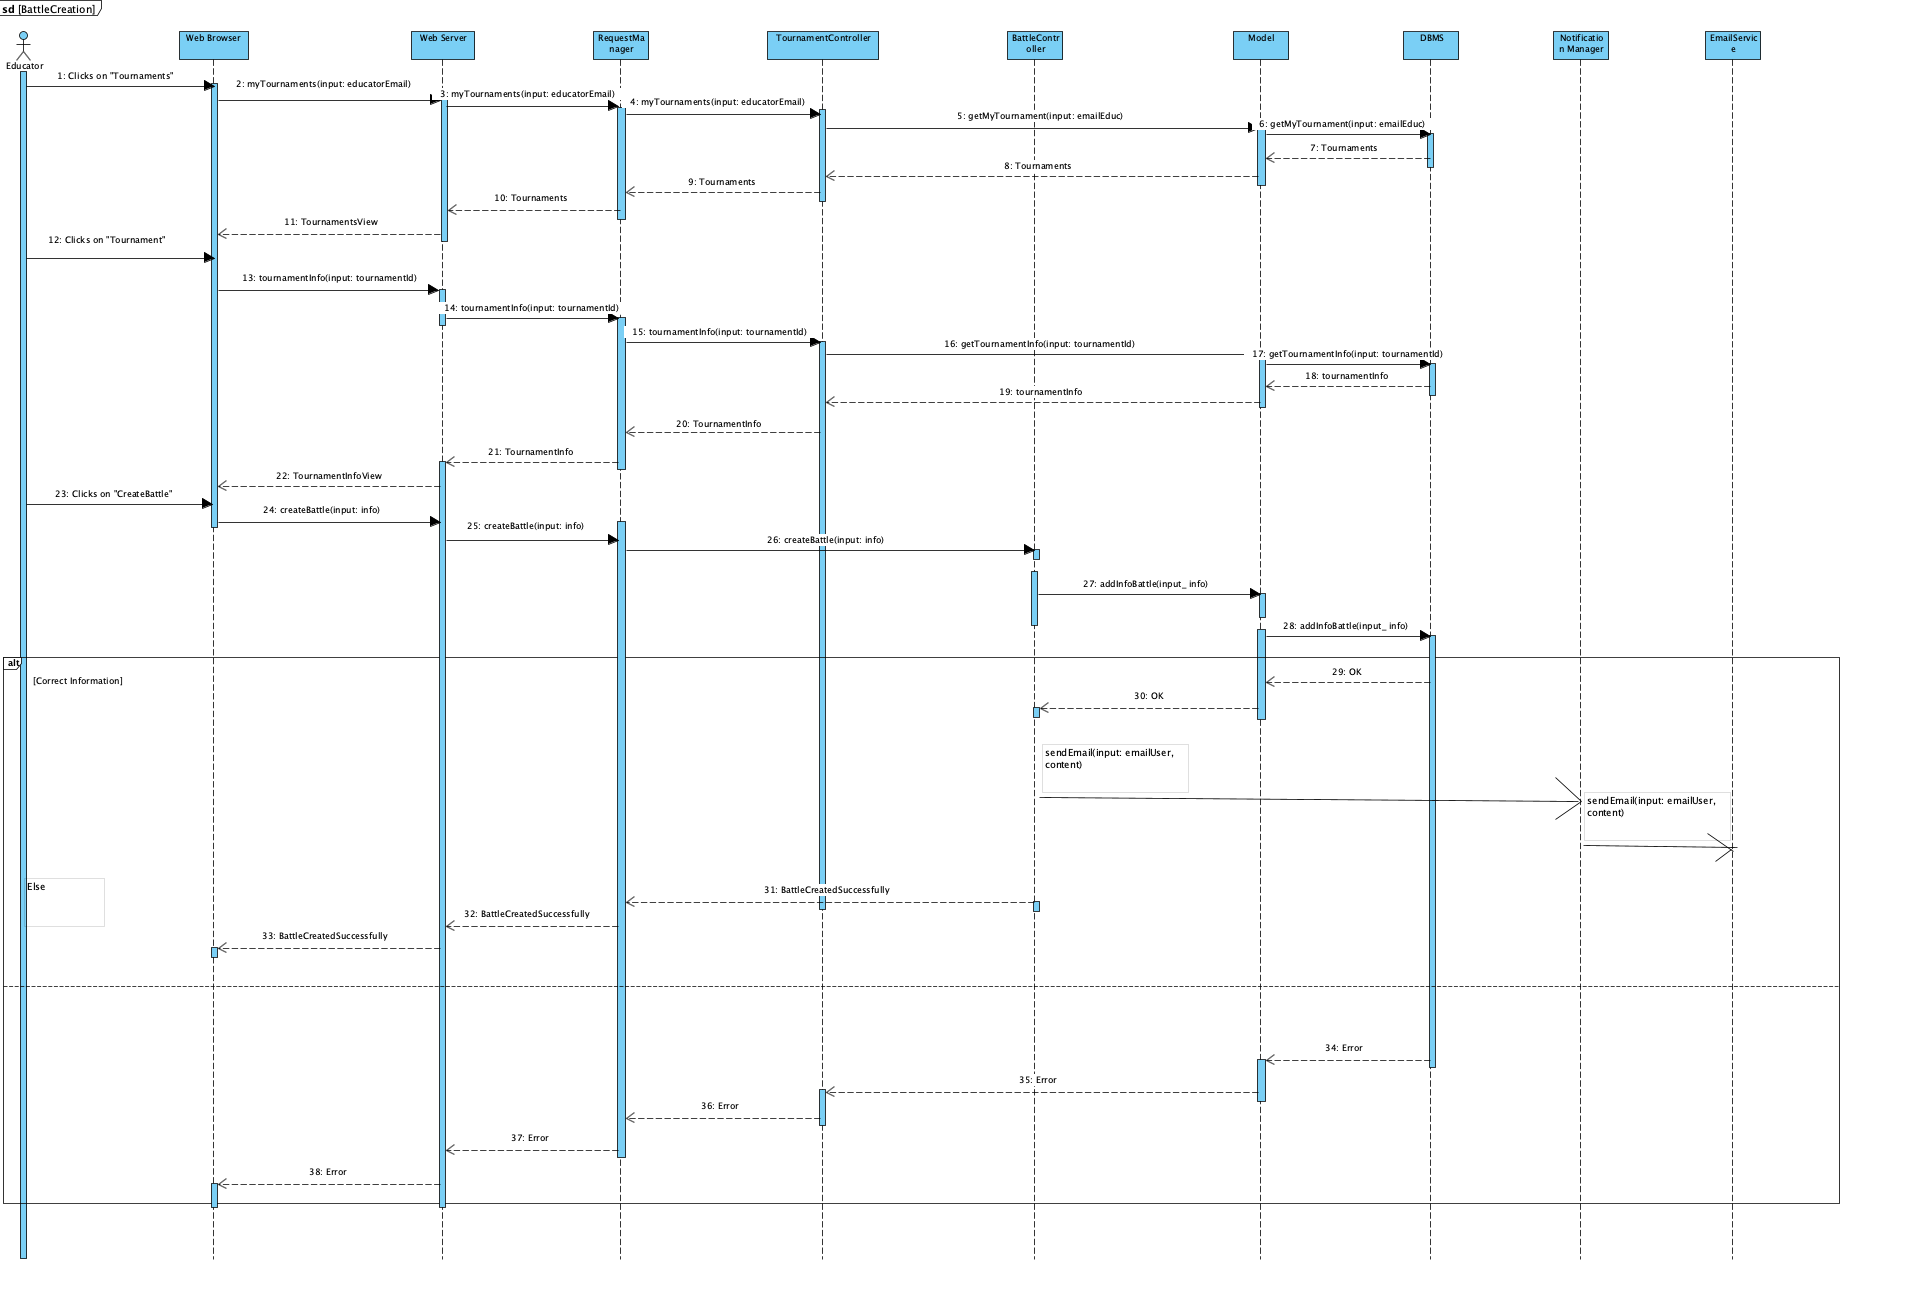
\includegraphics[width=1\linewidth]{SequenceDiagram/BattleCreation.png} 
  \caption{Battle creation}
  \label{fig:immagine}
\end{figure}


\newpage
%%%%USE CASE  ISCRIZIONE AL TORNO
\subsubsection{Student registers for the tournament}
\begin{longtable}{|c| p{10cm}|}
        \hline
            ID & 6 \\
        \hline
            Name & Student registers for the tournament  \\
        \hline
            Actor & Student \\
        \hline
            Entry Conditions & 
                          
                        The student  has logged in the system.\\
                                   
                    
        \hline
            Events Flow &   \begin{enumerate}
            
                                \item The student clicks on the "Tournaments" section of the dashboard
                                \item The system displays the page containing the list of available tournaments
                                \item The student browses through the list  and selects one he is interested in.
                                \item The system displays the specific tournament page.
                                \item The student clicks on the "Register" button to begin the registration process. 
                                \item The student successfully registers for a tournament.
                                
                            \end{enumerate} \\
        \hline
            Exit Conditions &
 
                                    The student receives a confirmation message, confirming their participation in the tournament and the system updates the database, recording the student’s participation in the tournament.
                                \\
        \hline
            Exceptions & 
                 If the registration for the tournament is closed or the tournament is closed , the student will simply not be allowed to register.
            \\
        \hline
    \end{longtable}
    \begin{figure}[H]
  %\centering
  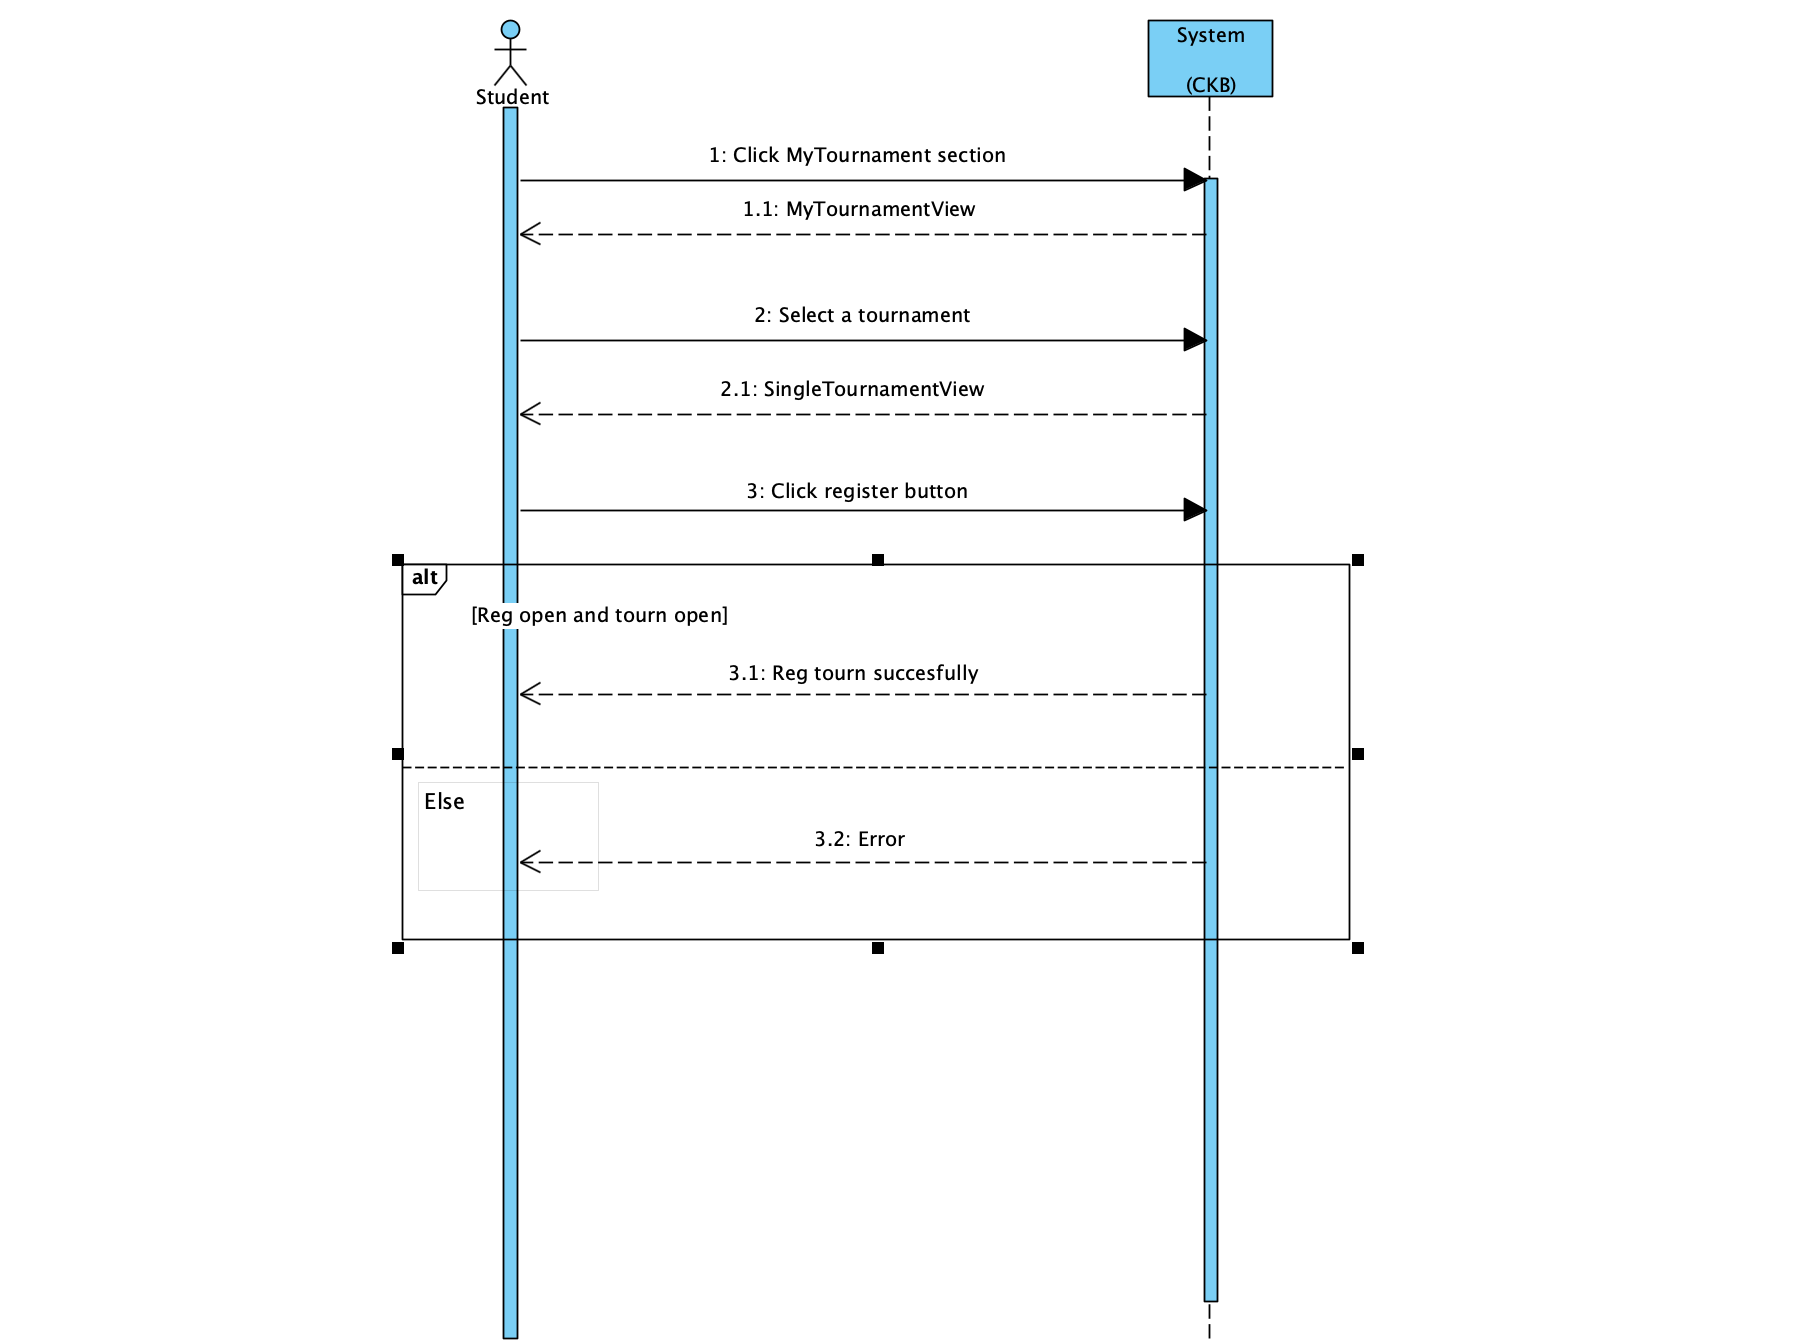
\includegraphics[width=1\linewidth]{SequenceDiagram/StudRegTourn.png} 
  \caption{Student registers for the tournament}
  \label{fig:immagine}
\end{figure}

%%USE CASE ISCRIZIONE ALLA BATTAGLIA

\newpage
\subsubsection{Student registers for the battle}
\begin{longtable}{|c| p{10cm}|}
        \hline
            ID & 7 \\
        \hline
            Name & Student registers for the battle  \\
        \hline
            Actor & Student \\
        \hline
            Entry Conditions & 
                                    The student  has logged in the system.
\\
        \hline
            Events Flow &   \begin{enumerate}
                
                                \item The student clicks on the "My tournament" section to view all the tournaments in which he is registered.
                                \item The system displays the page containing the list of the tournament in which the student is subscribed.
                                \item The student selects a tournament from within the "My tournament" section.

                                \item The system displays the specific tournament page.
                                \item Within the tournament, the student reviews available battles and selects the one they wish to participate in.
                                \item  The system displays the specific battle section.
                                \item The student reads through the battle details, the code kata description, deadlines, and specific rules or requirements. 
                                \item The student clicks on the “Register for Battle” button.
                                \item The system shows a section who allows student to invite other students to join his team and set information about the team.
                                \item  The student forms a team by inviting his friends.
                            \end{enumerate} \\
        \hline
            Exit Conditions &
                                     The student successfully registers for the selected battle, and the system updates the database, recording the team’s participation in the battle
                               \\
        \hline
            Exceptions & 
            \begin{itemize}
                \item If a student invites one or more students who are already participating in a team within that battle, the system displays an error message.
                \item If the registration for the battle is closed, the student will simply not be allowed to register.
                \item If the student tries to register for a battle in a tournament they are not enrolled in, the platform displays an error message explaining that they are not registered for the tournament.
                
            \end{itemize}\\
        \hline
    \end{longtable}
    \begin{figure}[H]
  %\centering
  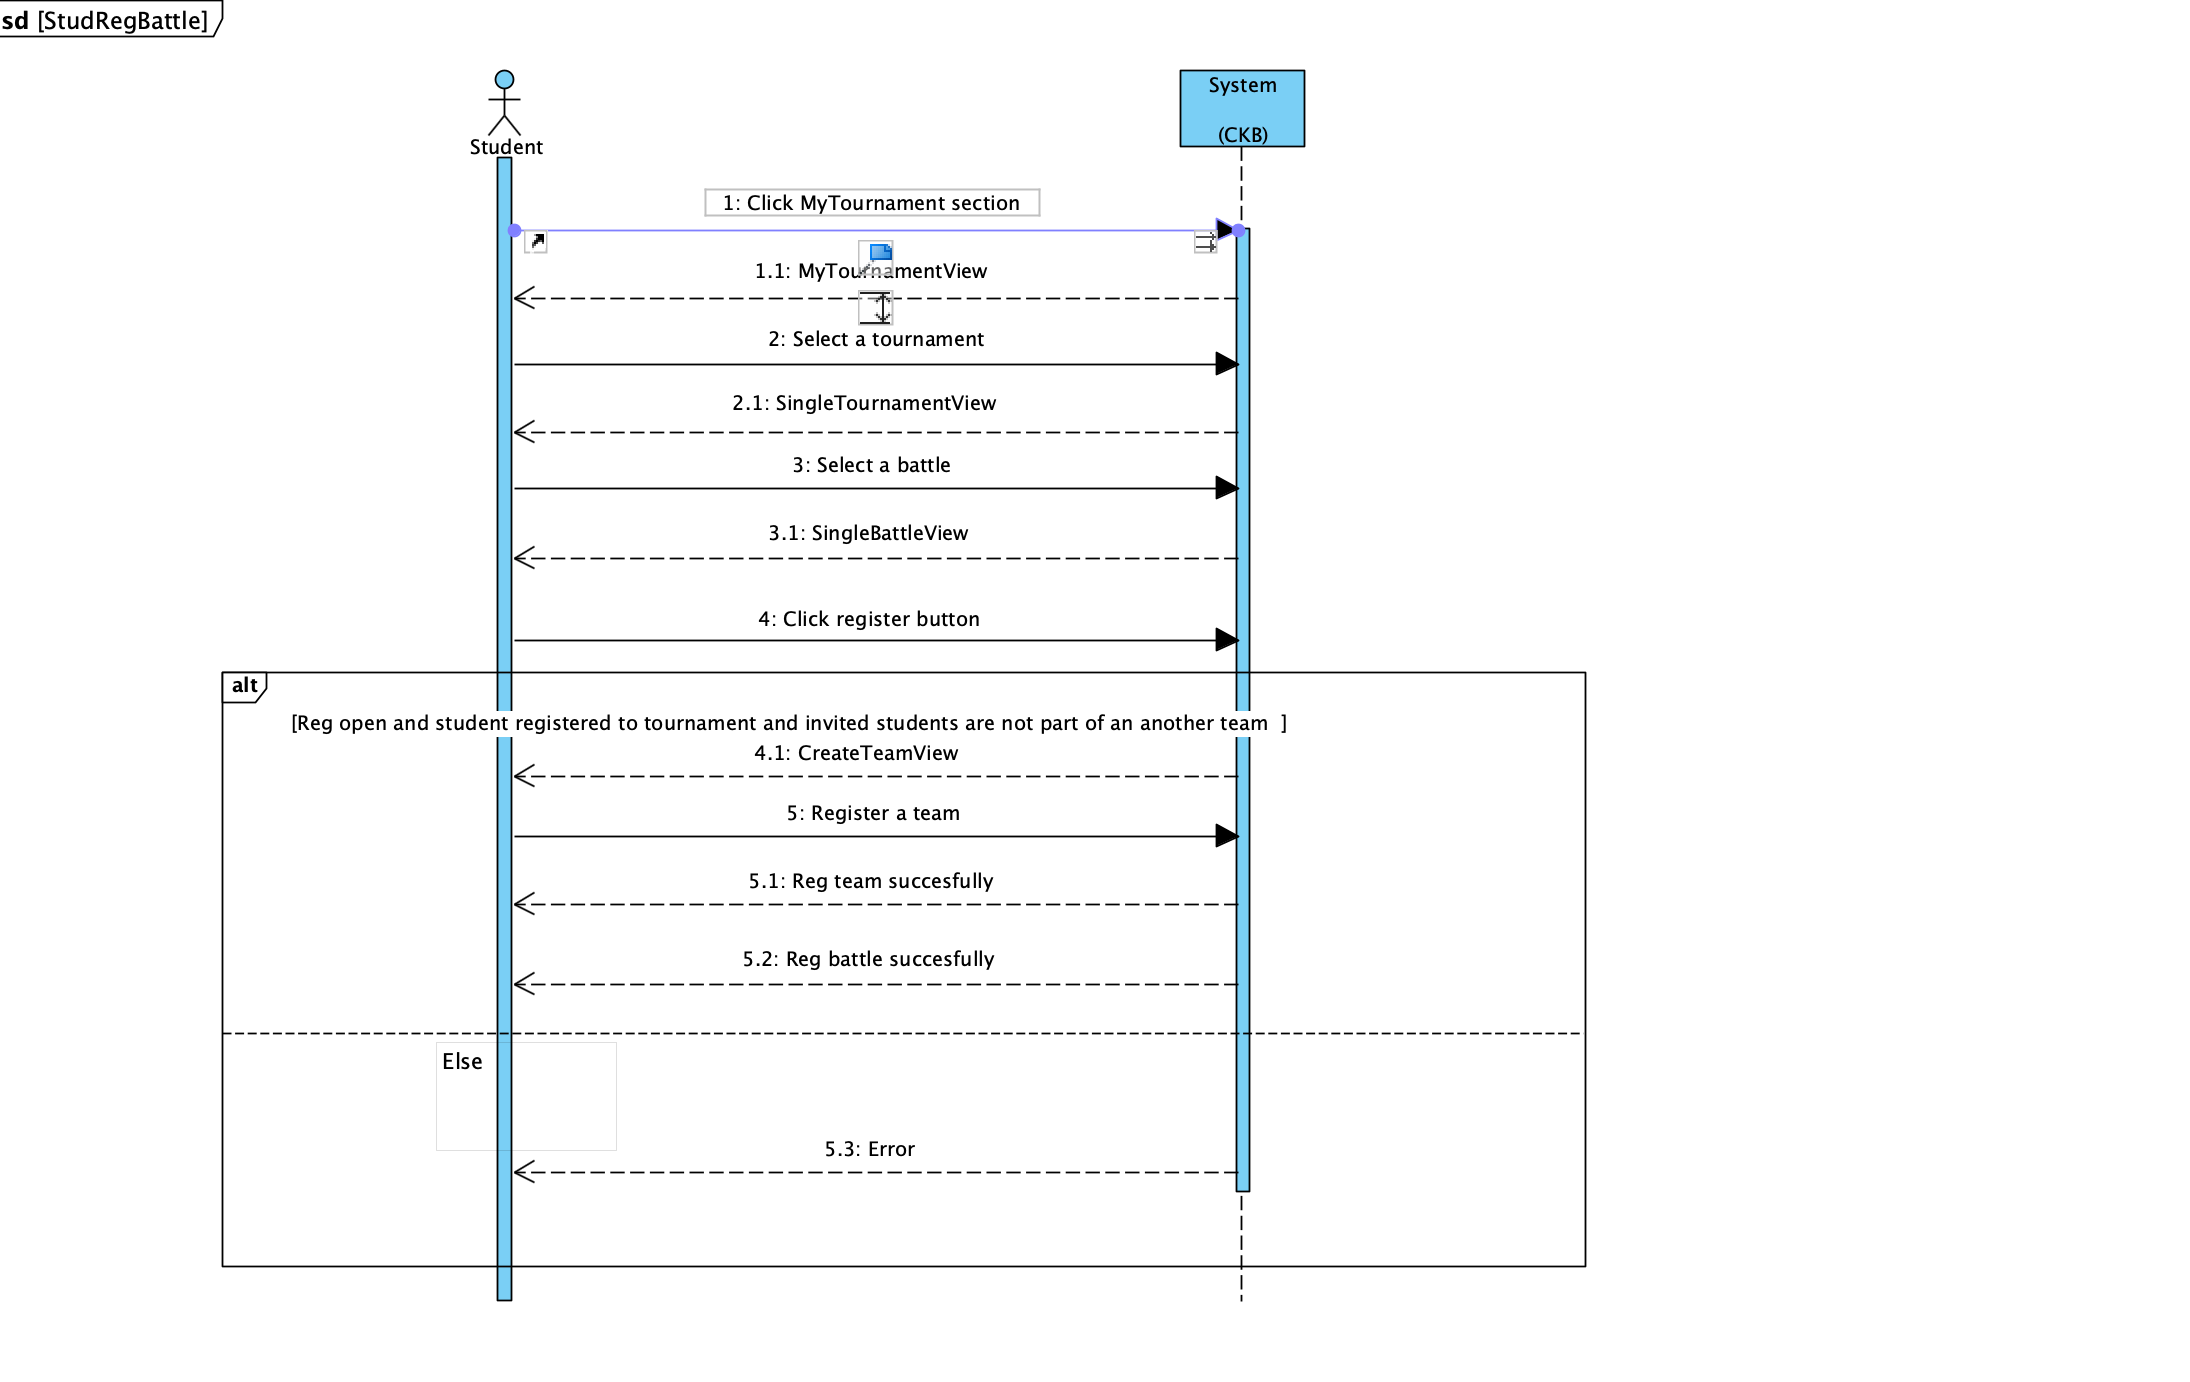
\includegraphics[width=1\linewidth]{SequenceDiagram/StudRegBattle.png} 
  \caption{Student registers for the battle}
  \label{fig:immagine}
\end{figure}


%% USE CASE FORMAZIONE TEAM
\subsubsection{Student invites other students to create a team}
\begin{longtable}{|c| p{10cm}|}
        \hline
            ID & 8 \\
        \hline
            Name & Student invite other student to create a team  \\
        \hline
            Actor & Student, email API \\
        \hline
            Entry Conditions & 

                                 The student has clicked "Register" for a specific battle on the platform and is at the section for  forming a team.
\\
        \hline
            Events Flow &   \begin{enumerate}
            
                                \item The student inserts a team name.
                                \item The student select the students  to form the team 
                                \item  The student click on "Create team"
                                
                            \end{enumerate} \\
        \hline
            Exit Conditions &
            The system creates team and notify all the students invited via email . 
\\
        \hline
    \end{longtable}

\begin{figure}[H]
  %\centering
  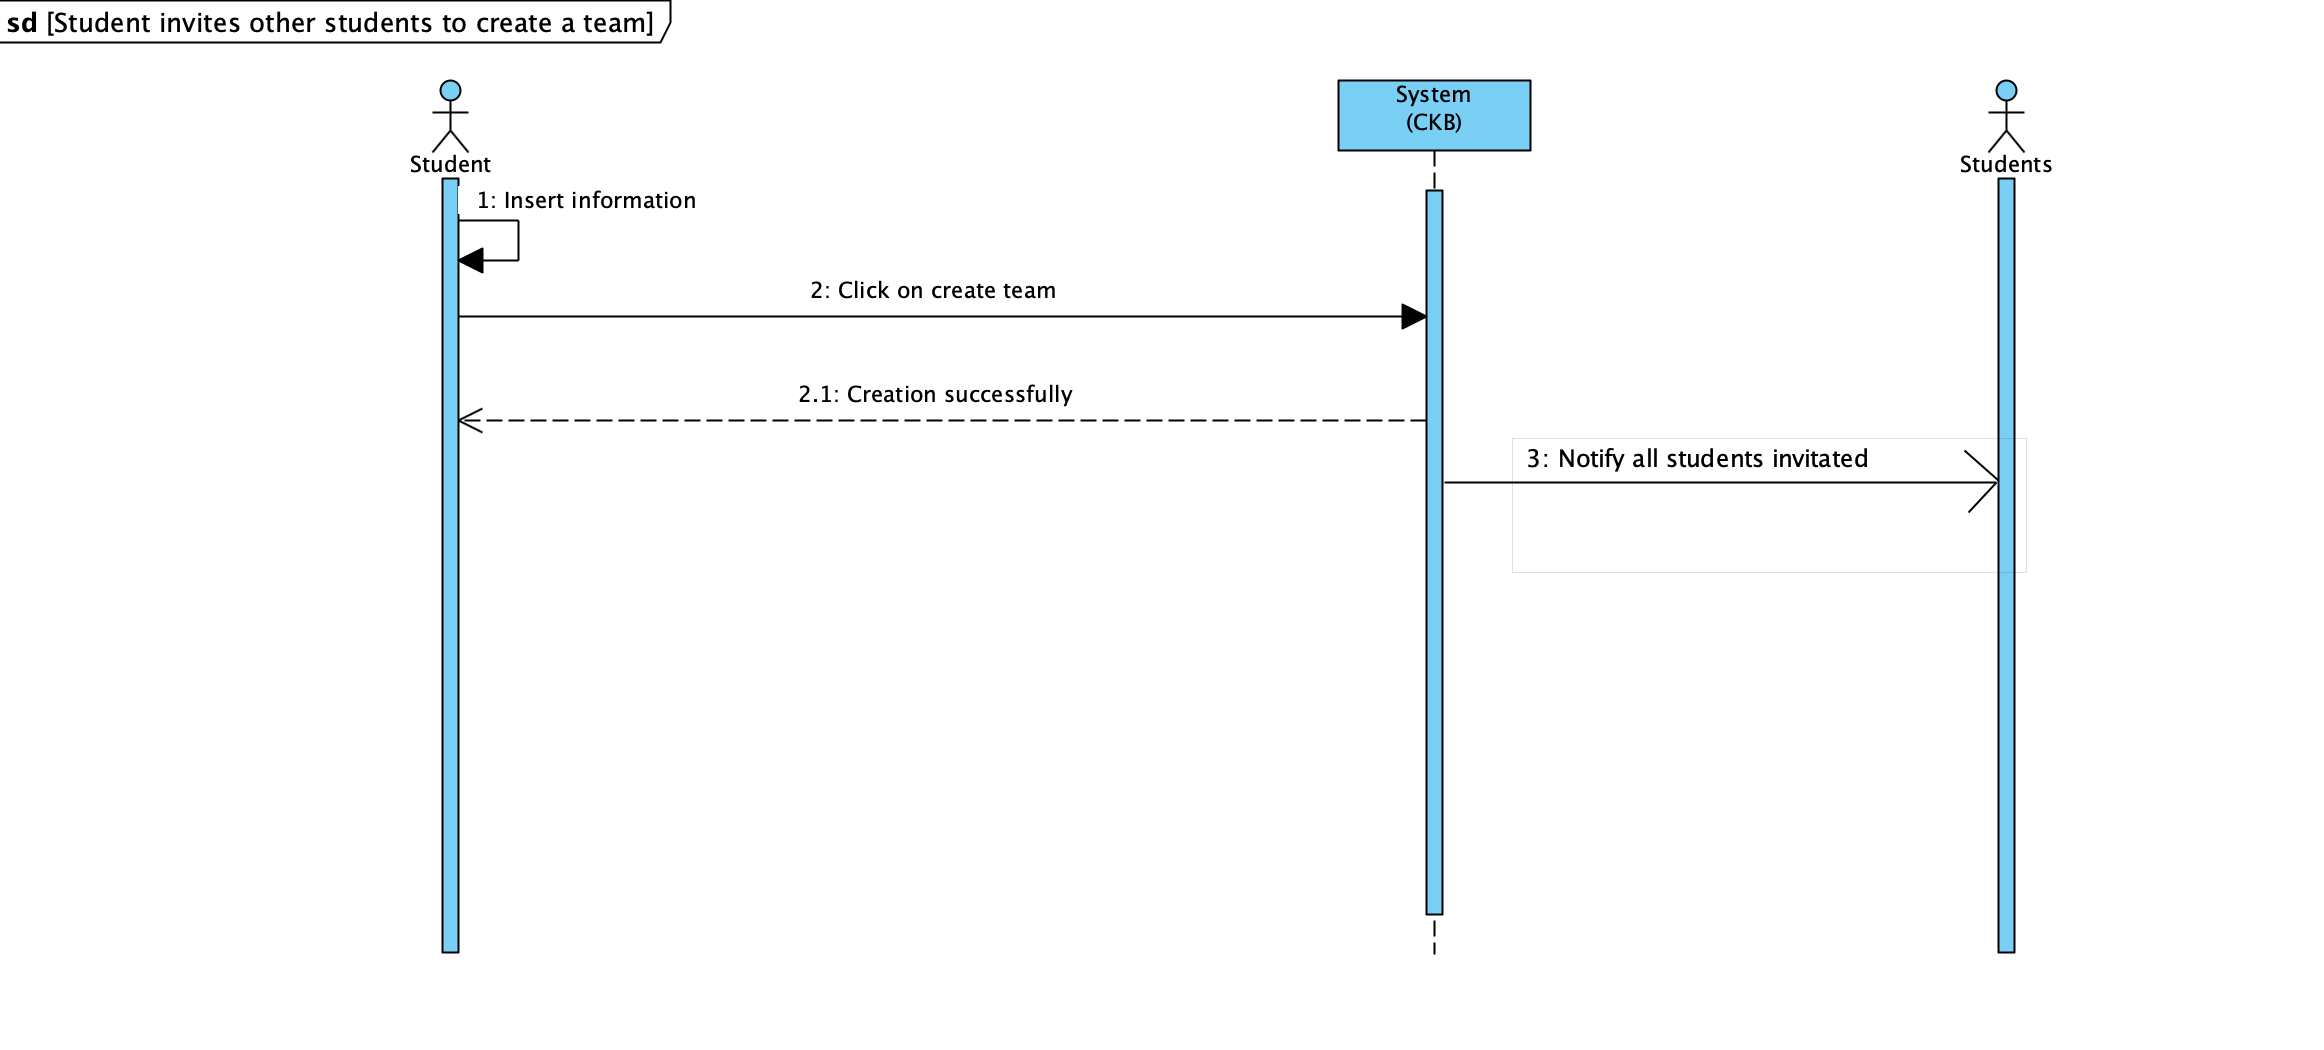
\includegraphics[width=1\linewidth]{SequenceDiagram/Invite.png} 
  \caption{Student invites other students to create a team}
  \label{fig:immagine}
\end{figure}


%%USE CASE ACCETTA INVITO DEL TEAM
\subsubsection{Students accept invitations and become part of the team}

\begin{longtable}{|c| p{10cm}|}
        \hline
            ID & 9 \\
        \hline
            Name & Students accept invitations and become part of the team \\
        \hline
            Actor & Student, email API \\
        \hline
            Entry Conditions & 

                                    The student  has logged in the system.
\\
        \hline
            Events Flow &   \begin{enumerate}
                
                                \item The students receive a link via email from the system.
                                \item  The students click on the link and is reported to CKB home page.
                                \item The system displays a confirmation message, in which the student can choose "Yes" to accept the invitation.
                                \item Once the students have accepted the invitation, they are ufficialy part of the team.
                                \item  System send a confirmation notifications via email to all team members.
                            \end{enumerate} \\
        \hline
            Exit Conditions &
            \begin{itemize}
                                    \item Students join the team and  system updates the database accordingly.
                                \end{itemize}\\
        \hline
            Exceptions & \begin{itemize}
                \item The students select "No" to decline the invitation. In this case, the system will notify the team's creator about this event.
                \item If the student tries to join a team for a battle in a tournament they are not enrolled in, the system displays an error message explaining that the user must first register for the tournament.
            \end{itemize} \\
        \hline
    \end{longtable}

\begin{figure}[H]
  %\centering
  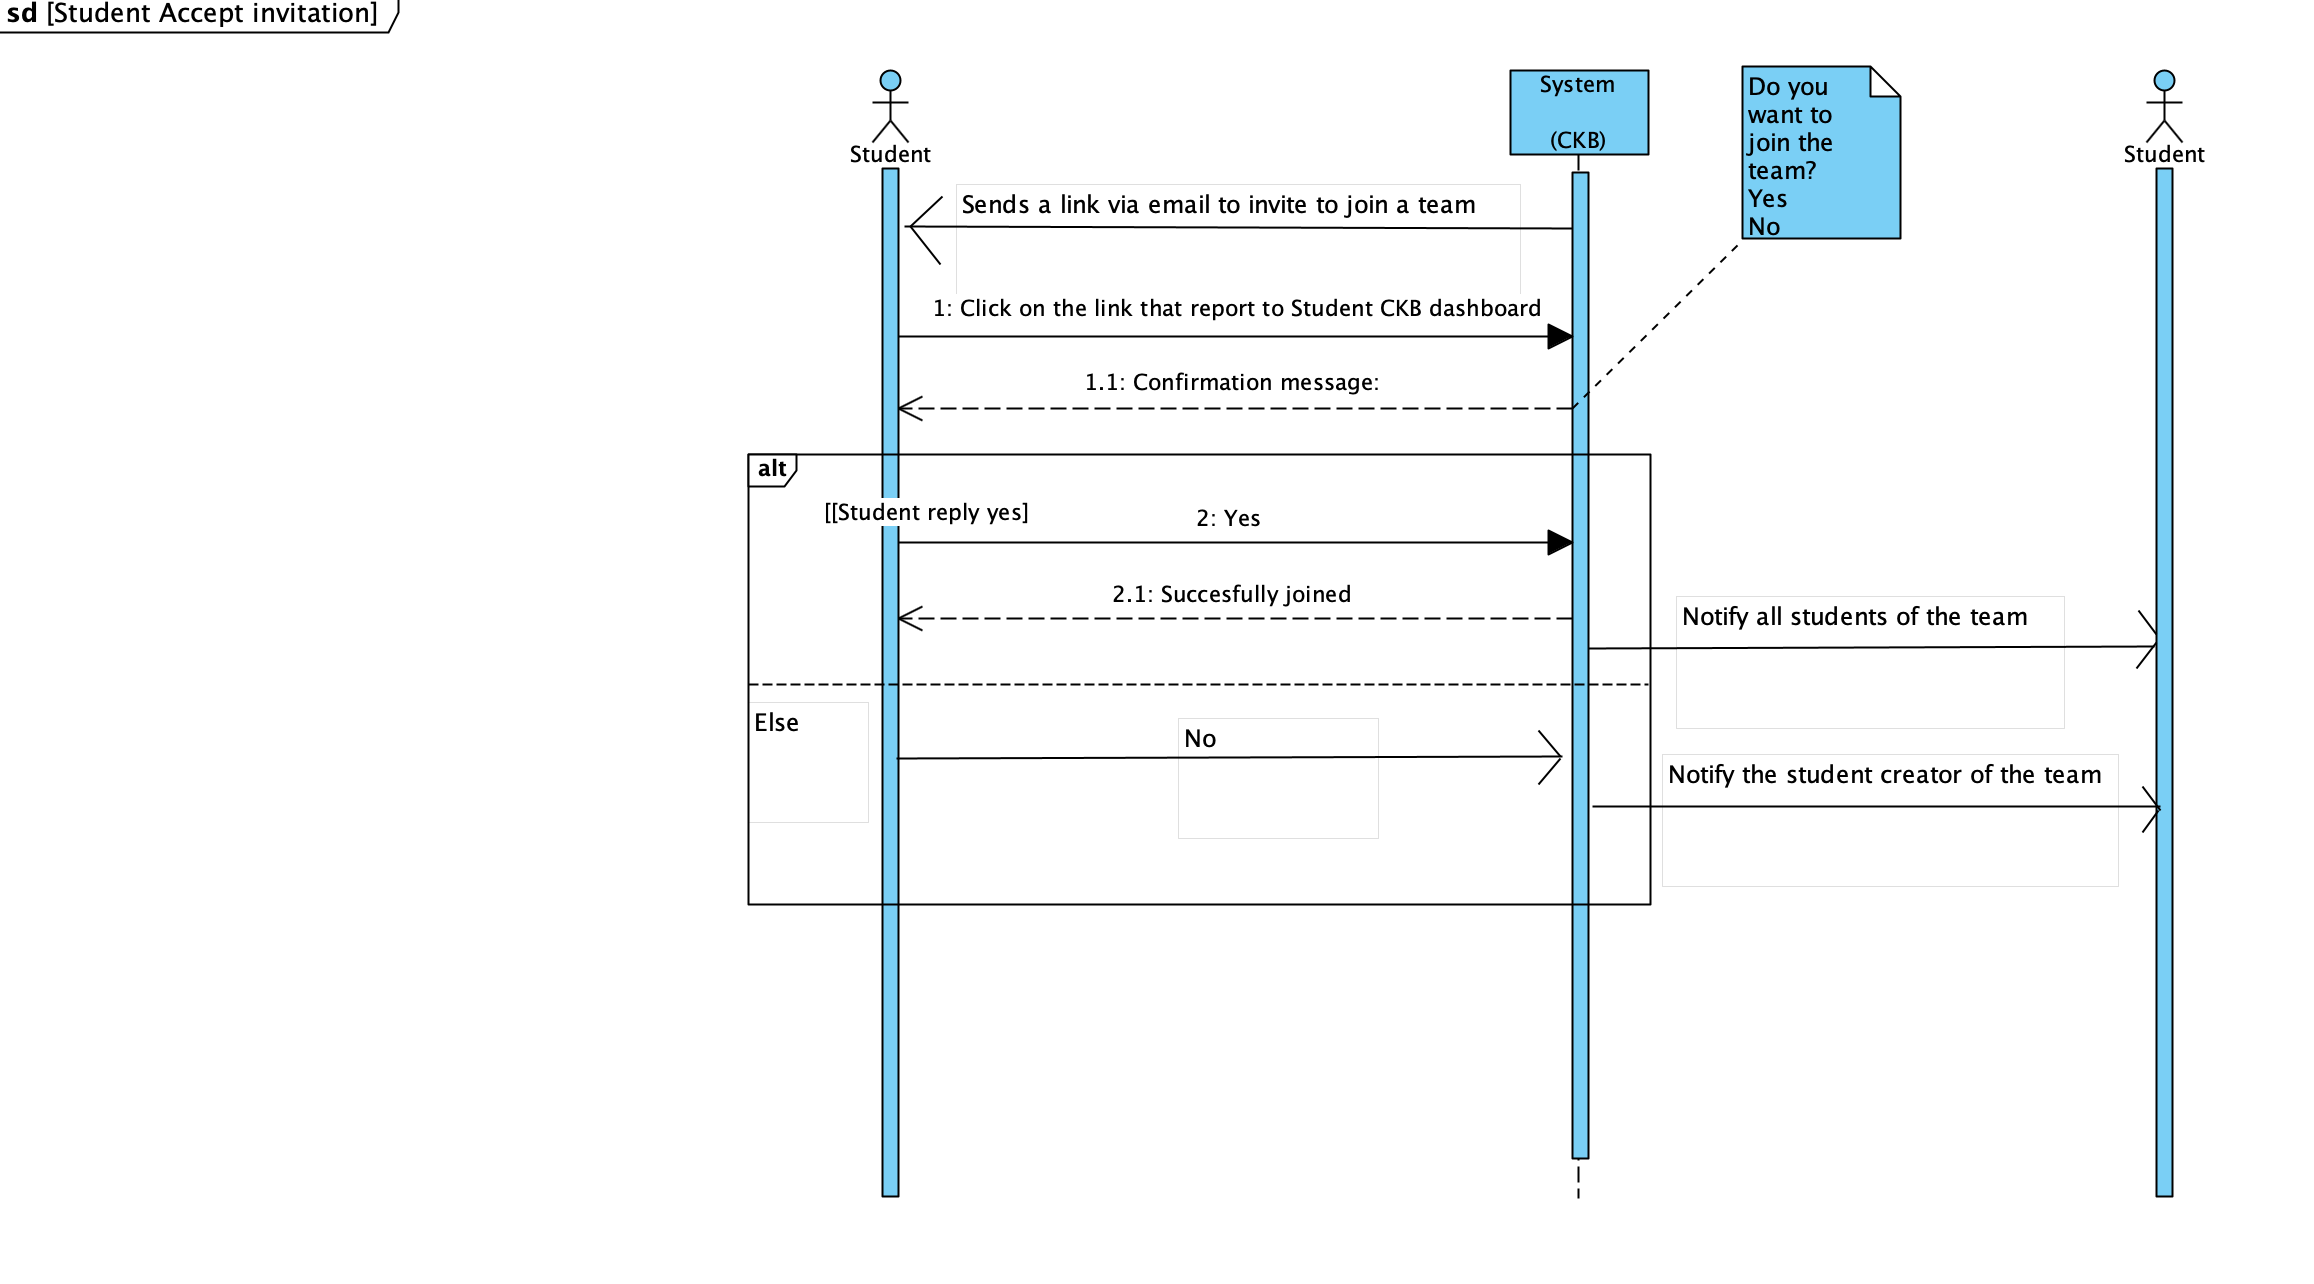
\includegraphics[width=1\linewidth]{SequenceDiagram/Students Accepts invitation.png} 
  \caption{Students accept invitations and become part of the team}
  \label{fig:immagine}
\end{figure}


\newpage
%%  USE CASE INIZIO DELLA BATTAGLIA
\subsubsection{Battle Setup}

\begin{longtable}{|c| p{10cm}|}
        \hline
            ID & 10 \\
        \hline
            Name & Battle Setup \\
        \hline
            Actor & Student, GitHub Actions \\
        \hline
            Entry Conditions & 
                     The registration deadline  for the battle expires
        
         \\
        \hline
            Events Flow &   \begin{enumerate}
                                \item The platform creates a GitHub repository containing the code kata(the project)
                                \item The system emails all students who have registered for the battle the link to the GitHub repository and instructions for setting up an automated workflow through GitHub Actions.
                                \item  Students fork the repository they've been sent
                                \item  Students  set up an automated workflow through GitHub Actions 
                            \end{enumerate} \\
                            \hline
            Exit Conditions &
    
                             
                                    The battle environment  is successfully setted up and  students start coding.
                                \\
        \hline
            
    \end{longtable}

    \begin{figure}[H]
  %\centering
  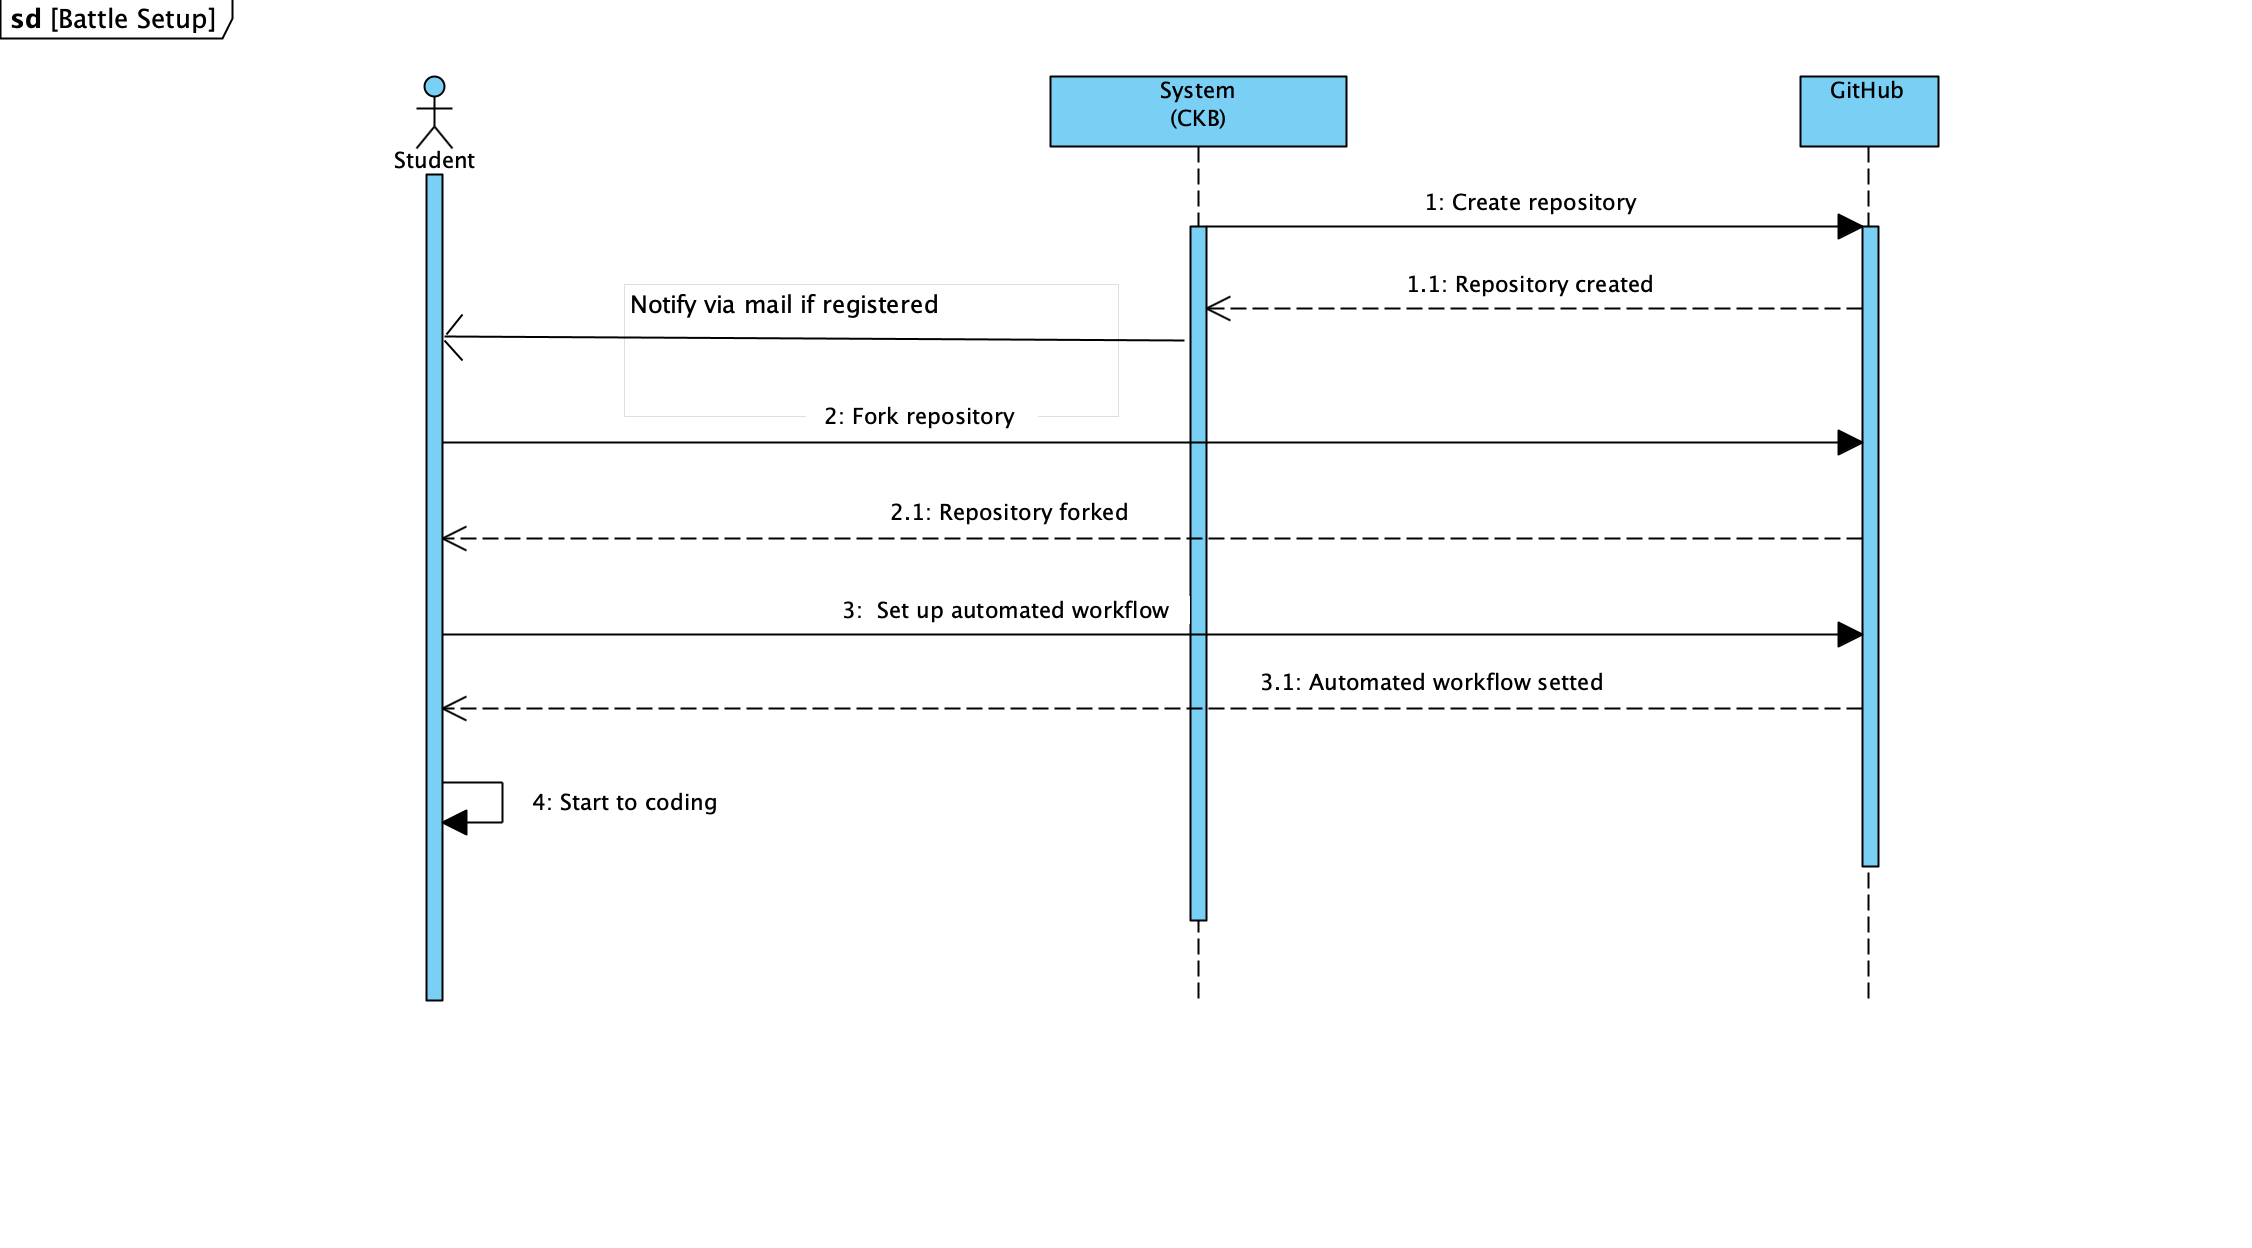
\includegraphics[width=1\linewidth]{SequenceDiagram/Battle setup.png} 
  \caption{Battle Setup}
  \label{fig:immagine}
\end{figure}




\newpage
\subsubsection{Students start to work}
\begin{longtable}{|c| p{10cm}|}
        \hline
            ID & 11 \\
        \hline
            Name & Students start to work \\
        \hline
            Actor & Student, GitHub Actions\\
        \hline
            Entry Conditions & 
              The battle environment has been successfully set up.
            
                     
        
         \\
        \hline
            Events Flow &   \begin{enumerate}
                              \item Students start coding the project 
                              \item Students commit to GitHub every time they want to update a change.
                                \item GitHub Actions notifies the CKB platform (via appropriate API calls) immediately when students push a new commit.
                                \item The CKB platform  pull the latest source code.
                                \item  The CKB platform calculates the team's score using automated tools configured during the battle creation
                                \item  The CKB platform updates the score of the team
                                \item Upon the submission deadline, the  platform stops monitoring for further pushes
                                \item The system close  the battle 
                            \end{enumerate} \\
                            \hline
            Exit Conditions &
    
                               The battle has been successfully concluded, and a consolidation process starts to finalize the scores.
                                \\
        \hline
            
    \end{longtable}

    \begin{figure}[H]
  %\centering
  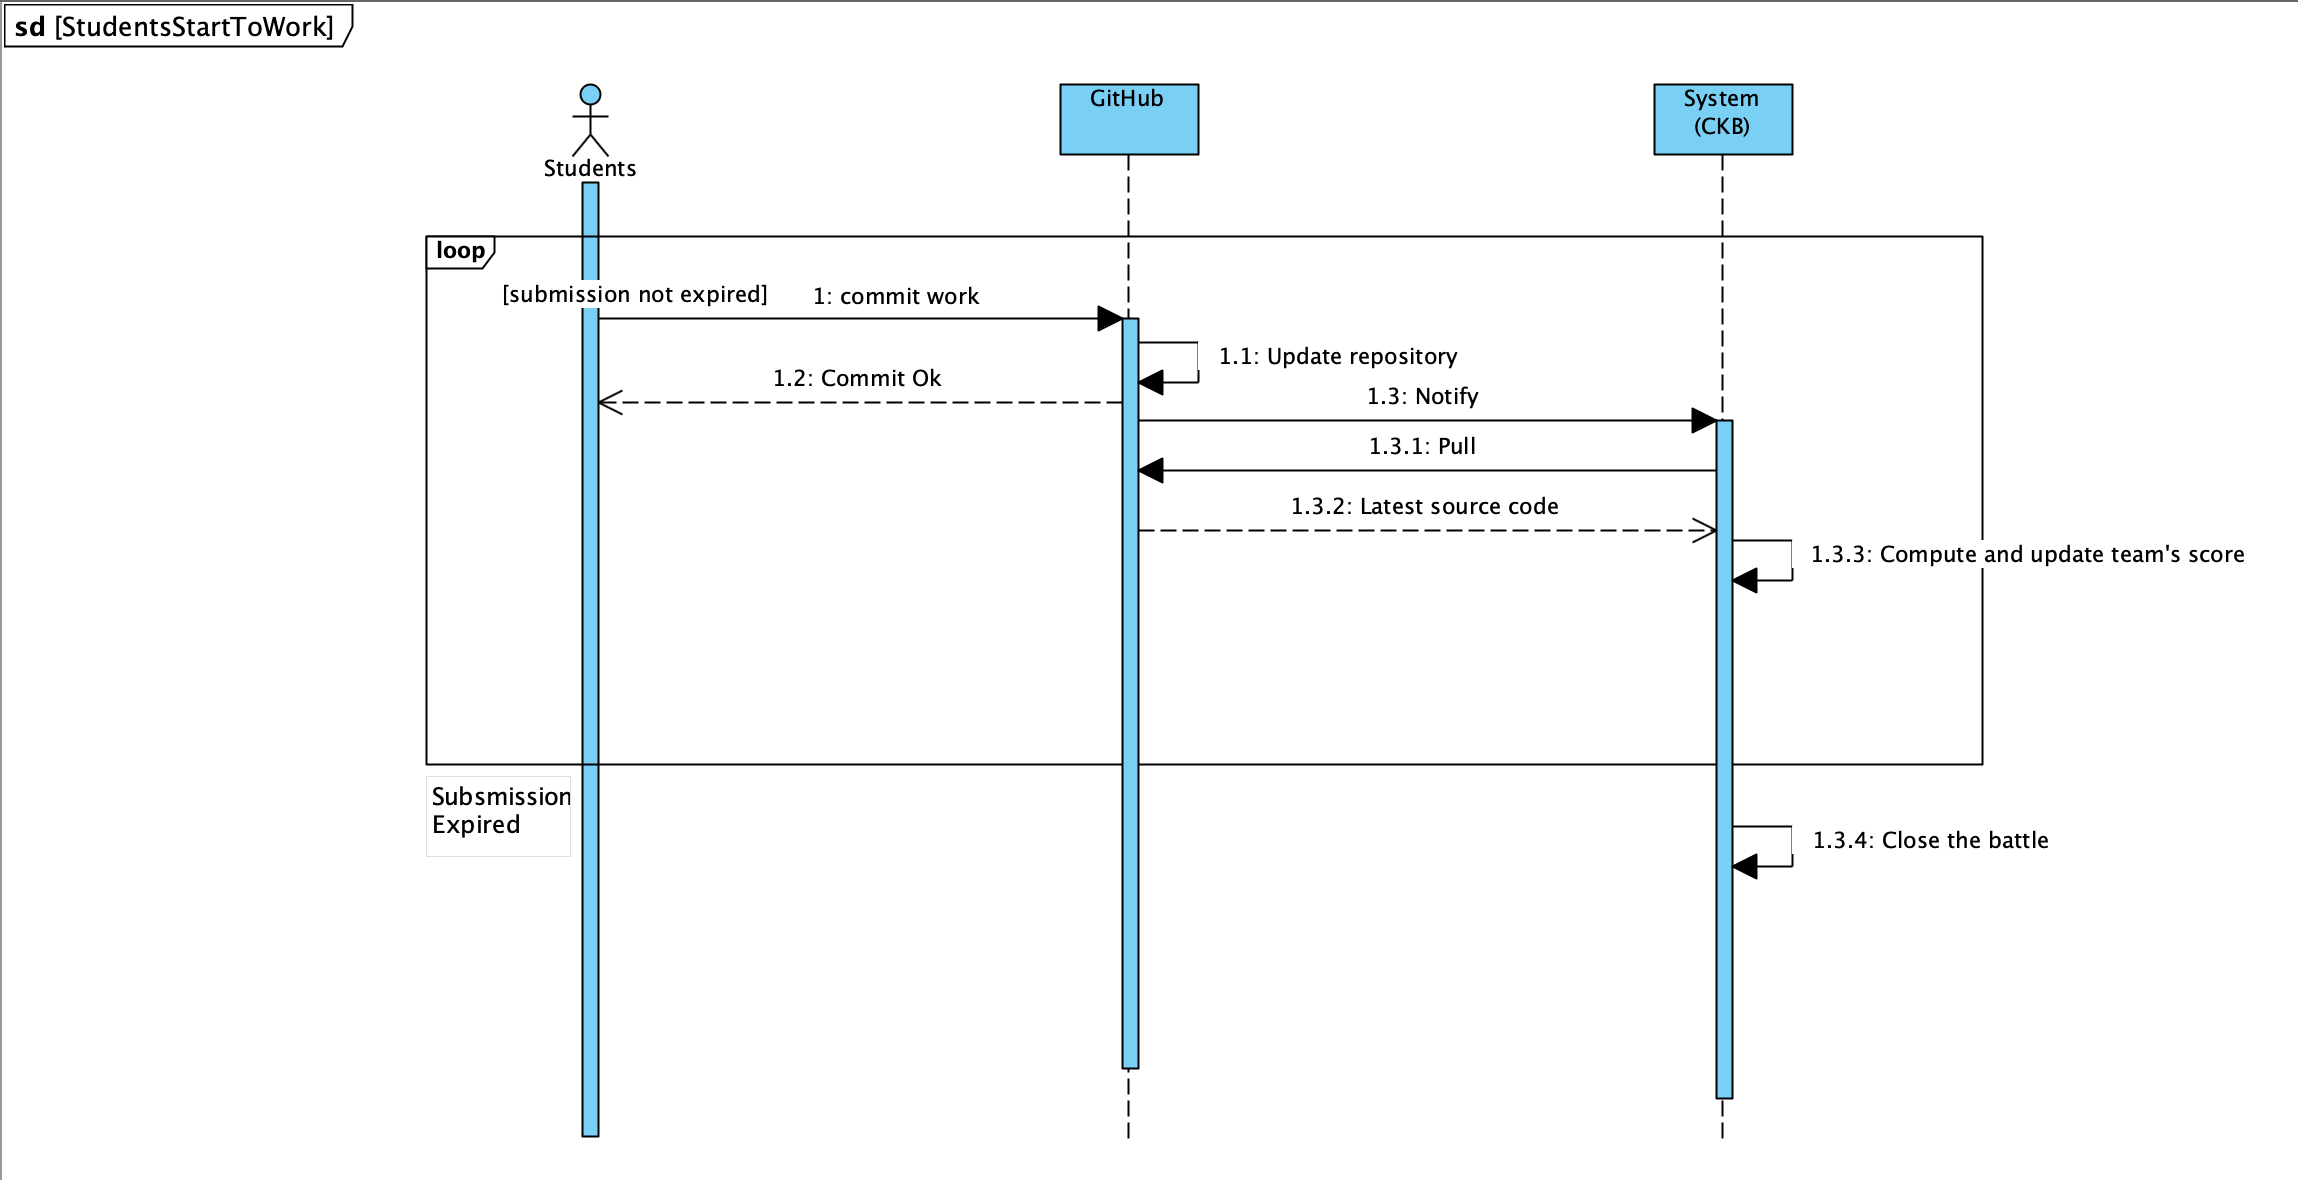
\includegraphics[width=1\linewidth]{SequenceDiagram/StudentsStartWorking.png} 
  \caption{Students start to work}
  \label{fig:immagine}
\end{figure}

\newpage
\subsubsection{Educator evaluation during the consolidation process}
\begin{longtable}{|c| p{10cm}|}
        \hline
            ID & 12 \\
        \hline
            Name & Educator evaluation during the consolidation process \\
        \hline
            Actor & Educator\\
        \hline
            Entry Conditions &
            The Code Kata Battle has reached its submission deadline
                

        
         \\
        \hline
            Events Flow &   \begin{enumerate}
                              \item The system updates all project files in the 'Final Submission' section of the respective Battle section.
                              \item Educator clicks on the "Final Submission" section 
                              \item The system displays "Final Submission" section
                              \item  Educator clicks on a project
                              \item The system open a new page referred to the project
                              \item The educator download the project by clicking on "Download".
                                \item The educator reviews the project and assigns a personal score (ranging from 0 to 100) to it.
                                \item Educator,after completing the review, click on "Submit evaluation".
                                \item  The educator repeats the process for all submitted projects.
                                \item The  platform calculates the final rankings by averaging the evaluations provided by educators and those generated through automated processes.
                            \end{enumerate} \\
                            \hline
            Exit Conditions & The platform notify via email   all students registered for the battle, informing them about the available rankings.
    
                             
                                \\
        \hline
         Exceptions & If manual evaluation is disabled, the platform will not upload the project to the 'Final Submission' section; instead, it will calculate the final rankings directly based on its automated evaluation.\\
             \hline
         
            
    \end{longtable}

\begin{figure}[H]
  %\centering
  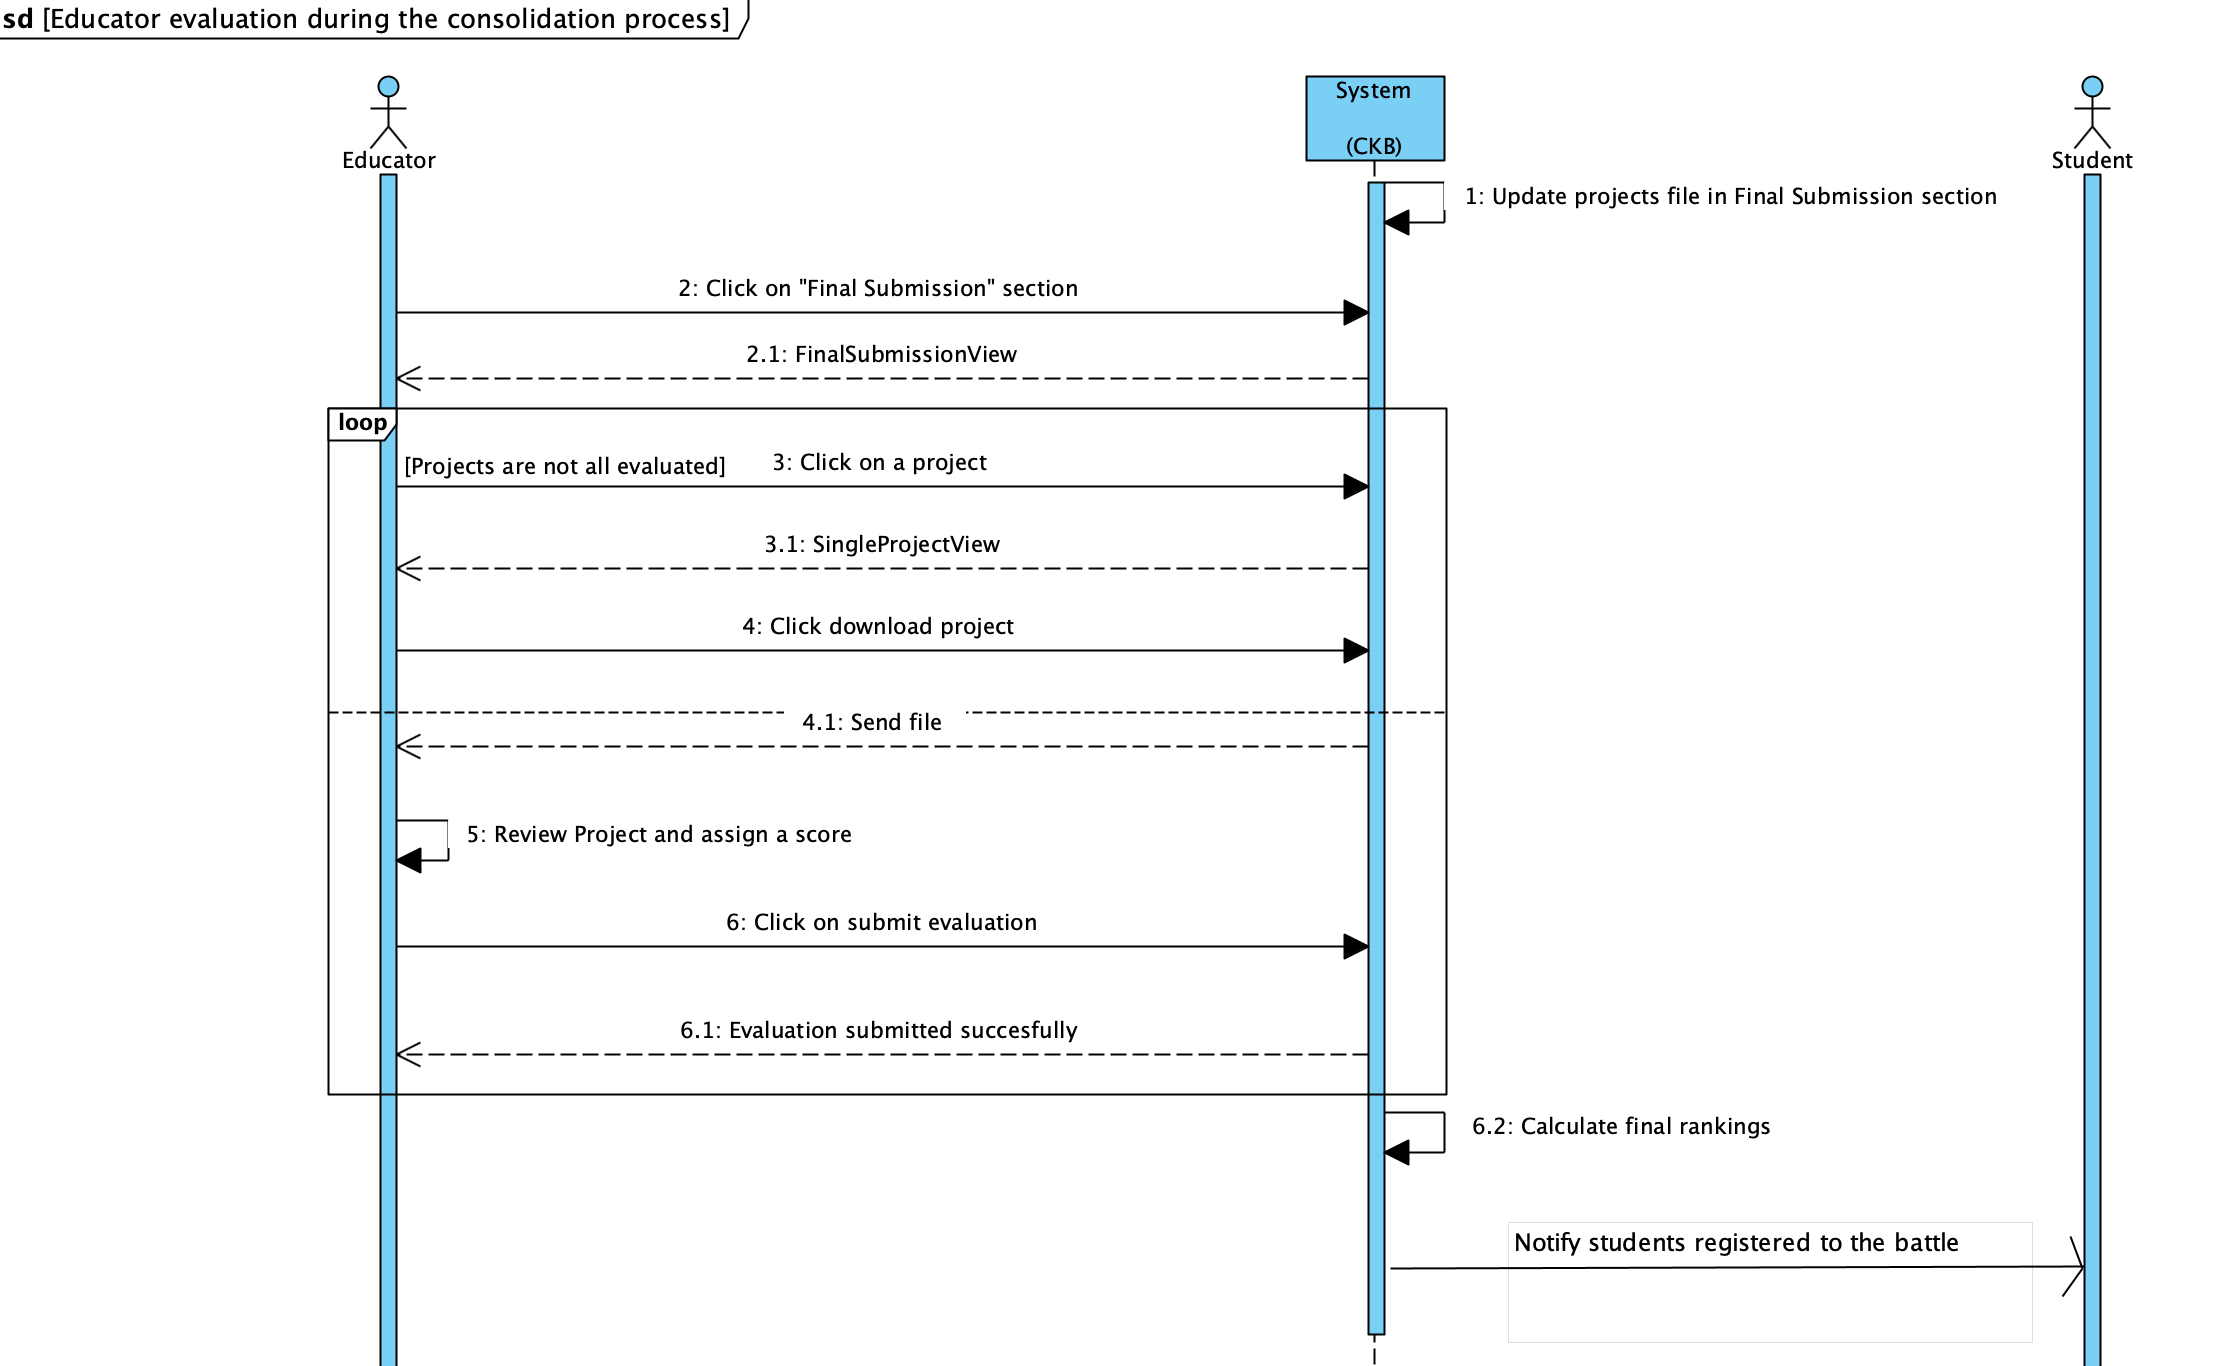
\includegraphics[width=1\linewidth]{SequenceDiagram/Educator evaluation during the consolidation process.png} 
  \caption{Educator evaluation during the consolidation process}
  \label{fig:immagine}
\end{figure}




\newpage
%% Educator monitors battle ranking
\subsubsection{Educator monitors battle ranking}

\begin{longtable}{|c| p{10cm}|}
    \hline
        ID & 13 \\
    \hline
        Name & Educator monitors battle ranking \\
    \hline
        Actor & Educator \\
    \hline
        Entry Conditions & 

                The educator has logged into the system.
\\
    \hline
        Events Flow &   \begin{enumerate}
                            \item The educator, through the homepage, clicks on the "Tournament" section.
                            \item The system presents a control dashboard that displays the tournaments created by the educator or those for which they have permission to organize battles.
                            \item The educator clicks on "All Tournaments".
                            \item The system displays a page that includes all tournaments of the platform, even those for which the educator does not have permission to create battles.
                            \item The educator clicks on a specific tournament.
                            \item The system displays the dashboard containing battles for the selected tournament to the educator.
                            \item The educator selects the battle they want to view the ranking of.
                        \end{enumerate} \\
    \hline
        Exit Conditions &

            The system displays the battle ranking to the educator, containing the following fields:
            \begin{itemize}
                                \item Team ID
                                \item Team name
                                \item Team Score calculated in real-time by the system
                            \end{itemize}
\\
    \hline
\end{longtable}

    \begin{figure}[H]
  %\centering
  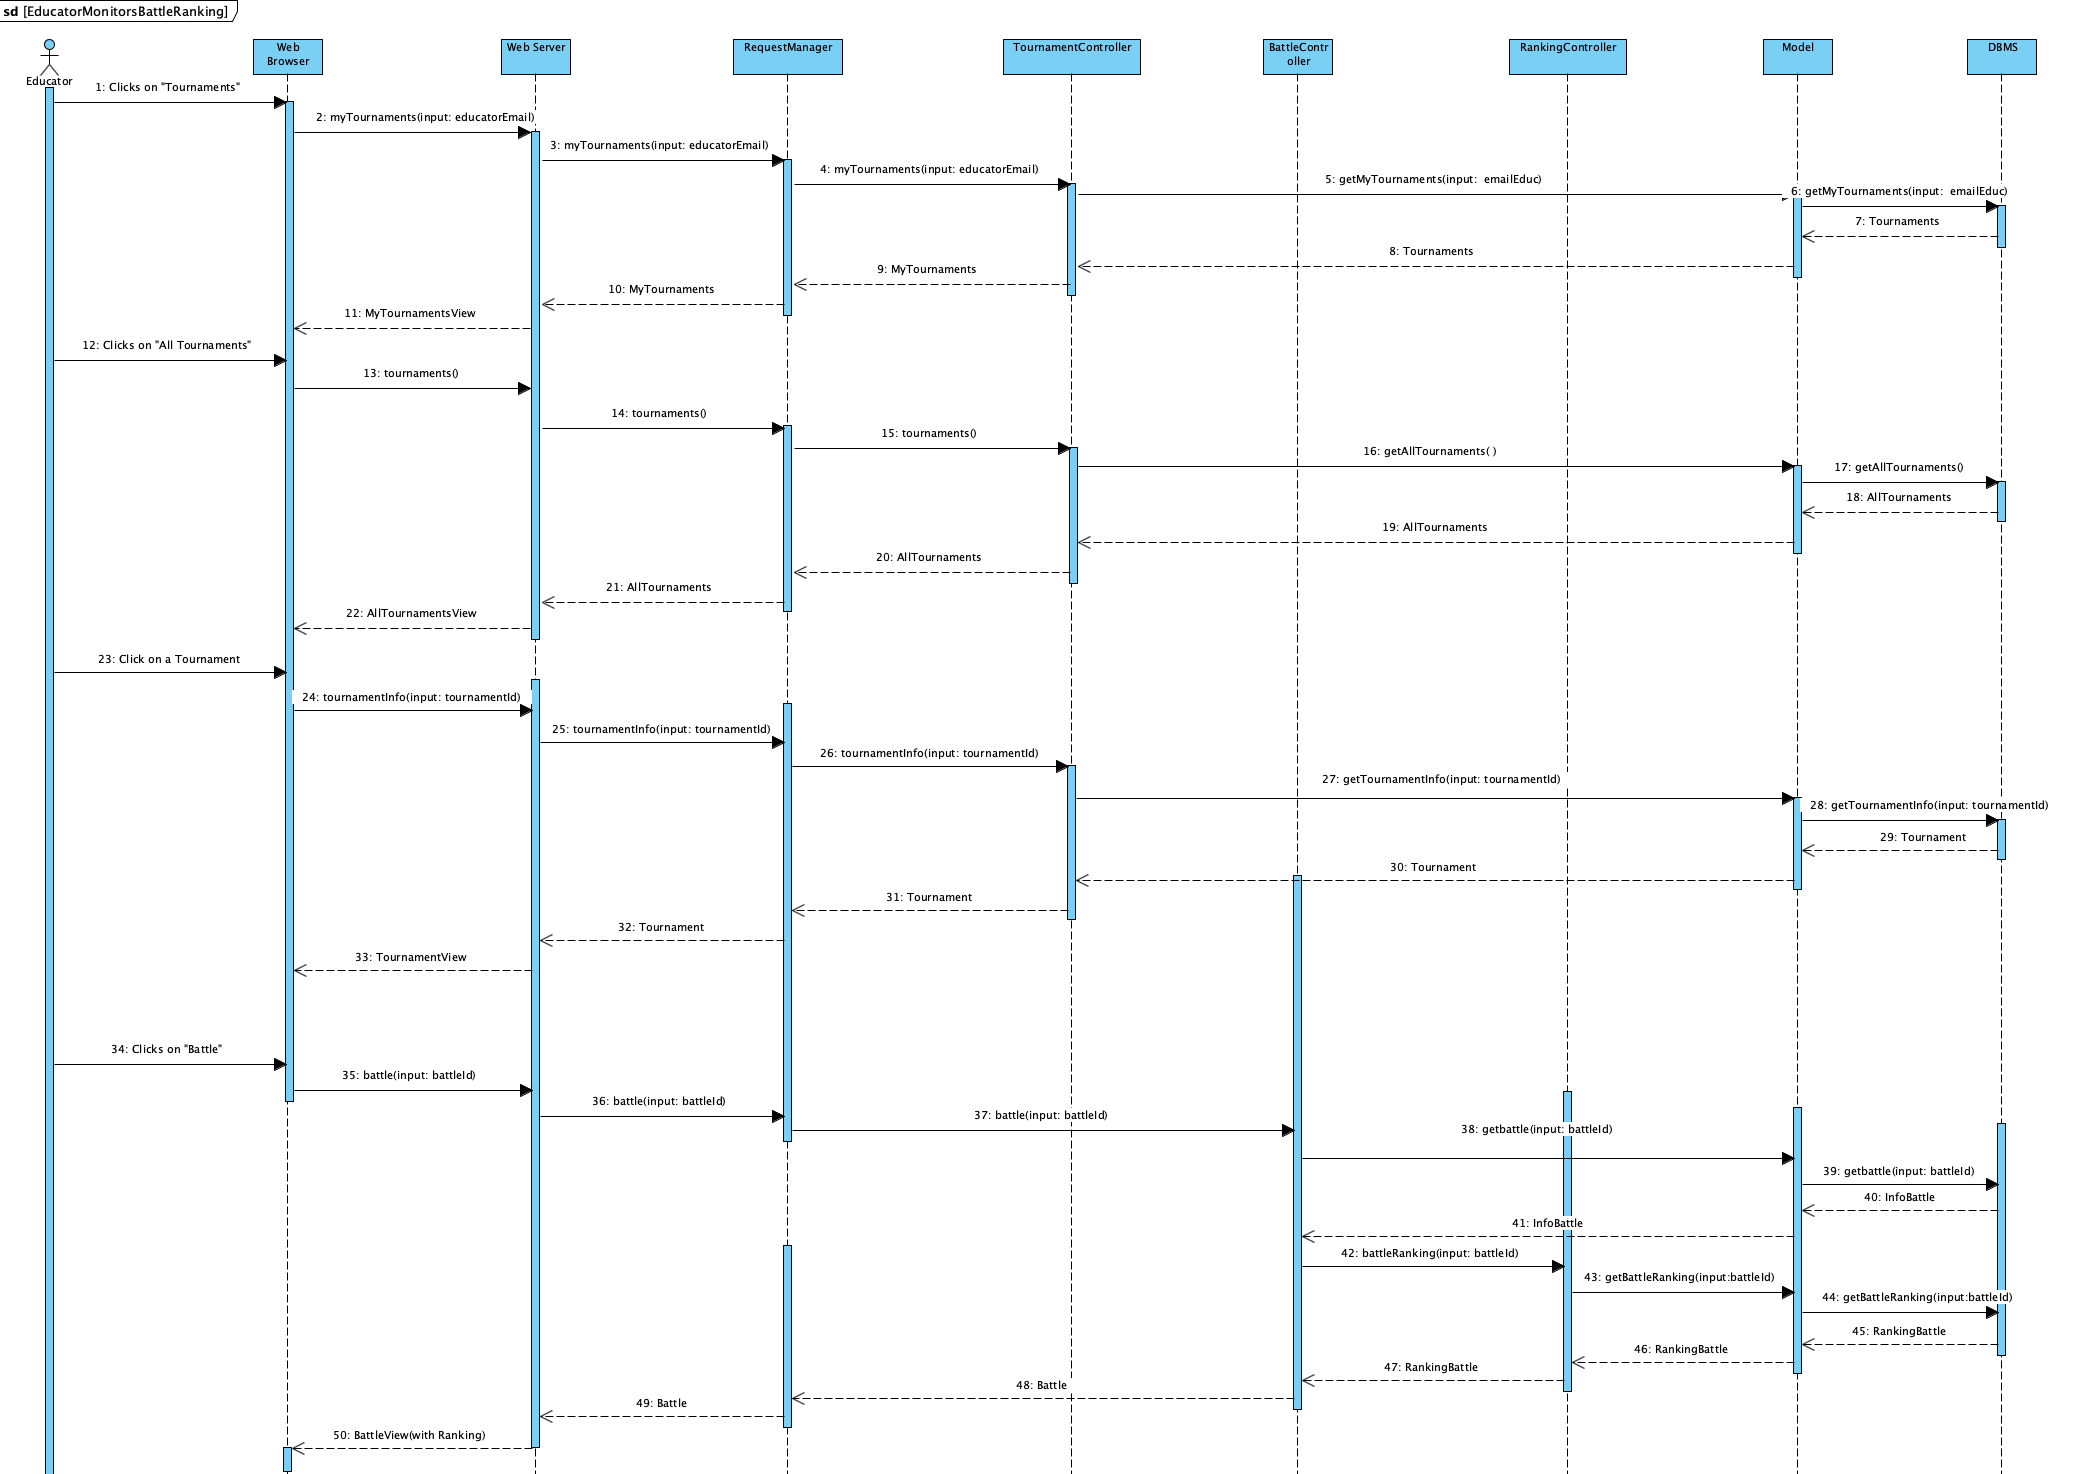
\includegraphics[width=1\linewidth]{SequenceDiagram/EducatorMonitorsBattleRanking.png} 
  \caption{Educator monitors battle ranking}
  \label{fig:immagine}
\end{figure}
%% Student monitors battle ranking

\newpage
\subsubsection{Student monitors battle ranking}

\begin{longtable}{|c| p{10cm}|}
    \hline
        ID & 14 \\
    \hline
        Name & Student monitors battle ranking \\
    \hline
        Actor & Student \\
    \hline
        Entry Conditions & 

                The student has logged into the system.
\\
    \hline
        Events Flow &   \begin{enumerate}
                            \item The student, through the homepage, clicks on the "Tournament" section.
                            \item The system presents a list of all the tournaments available on the platform.
                            \item The student clicks on a specific tournament.
                            \item The system displays the dashboard containing battles for the selected tournament to the student.
                            \item The student selects the battle they want to view the ranking of.
                        \end{enumerate} \\
    \hline
        Exit Conditions &

The system displays the battle ranking to the student, containing the following fields:
            \begin{itemize}
                                \item Team ID
                                \item Team name
                                \item Team Score calculated in real-time by the system
                            \end{itemize}
\\
    \hline
\end{longtable}

    \begin{figure}[H]
  %\centering
  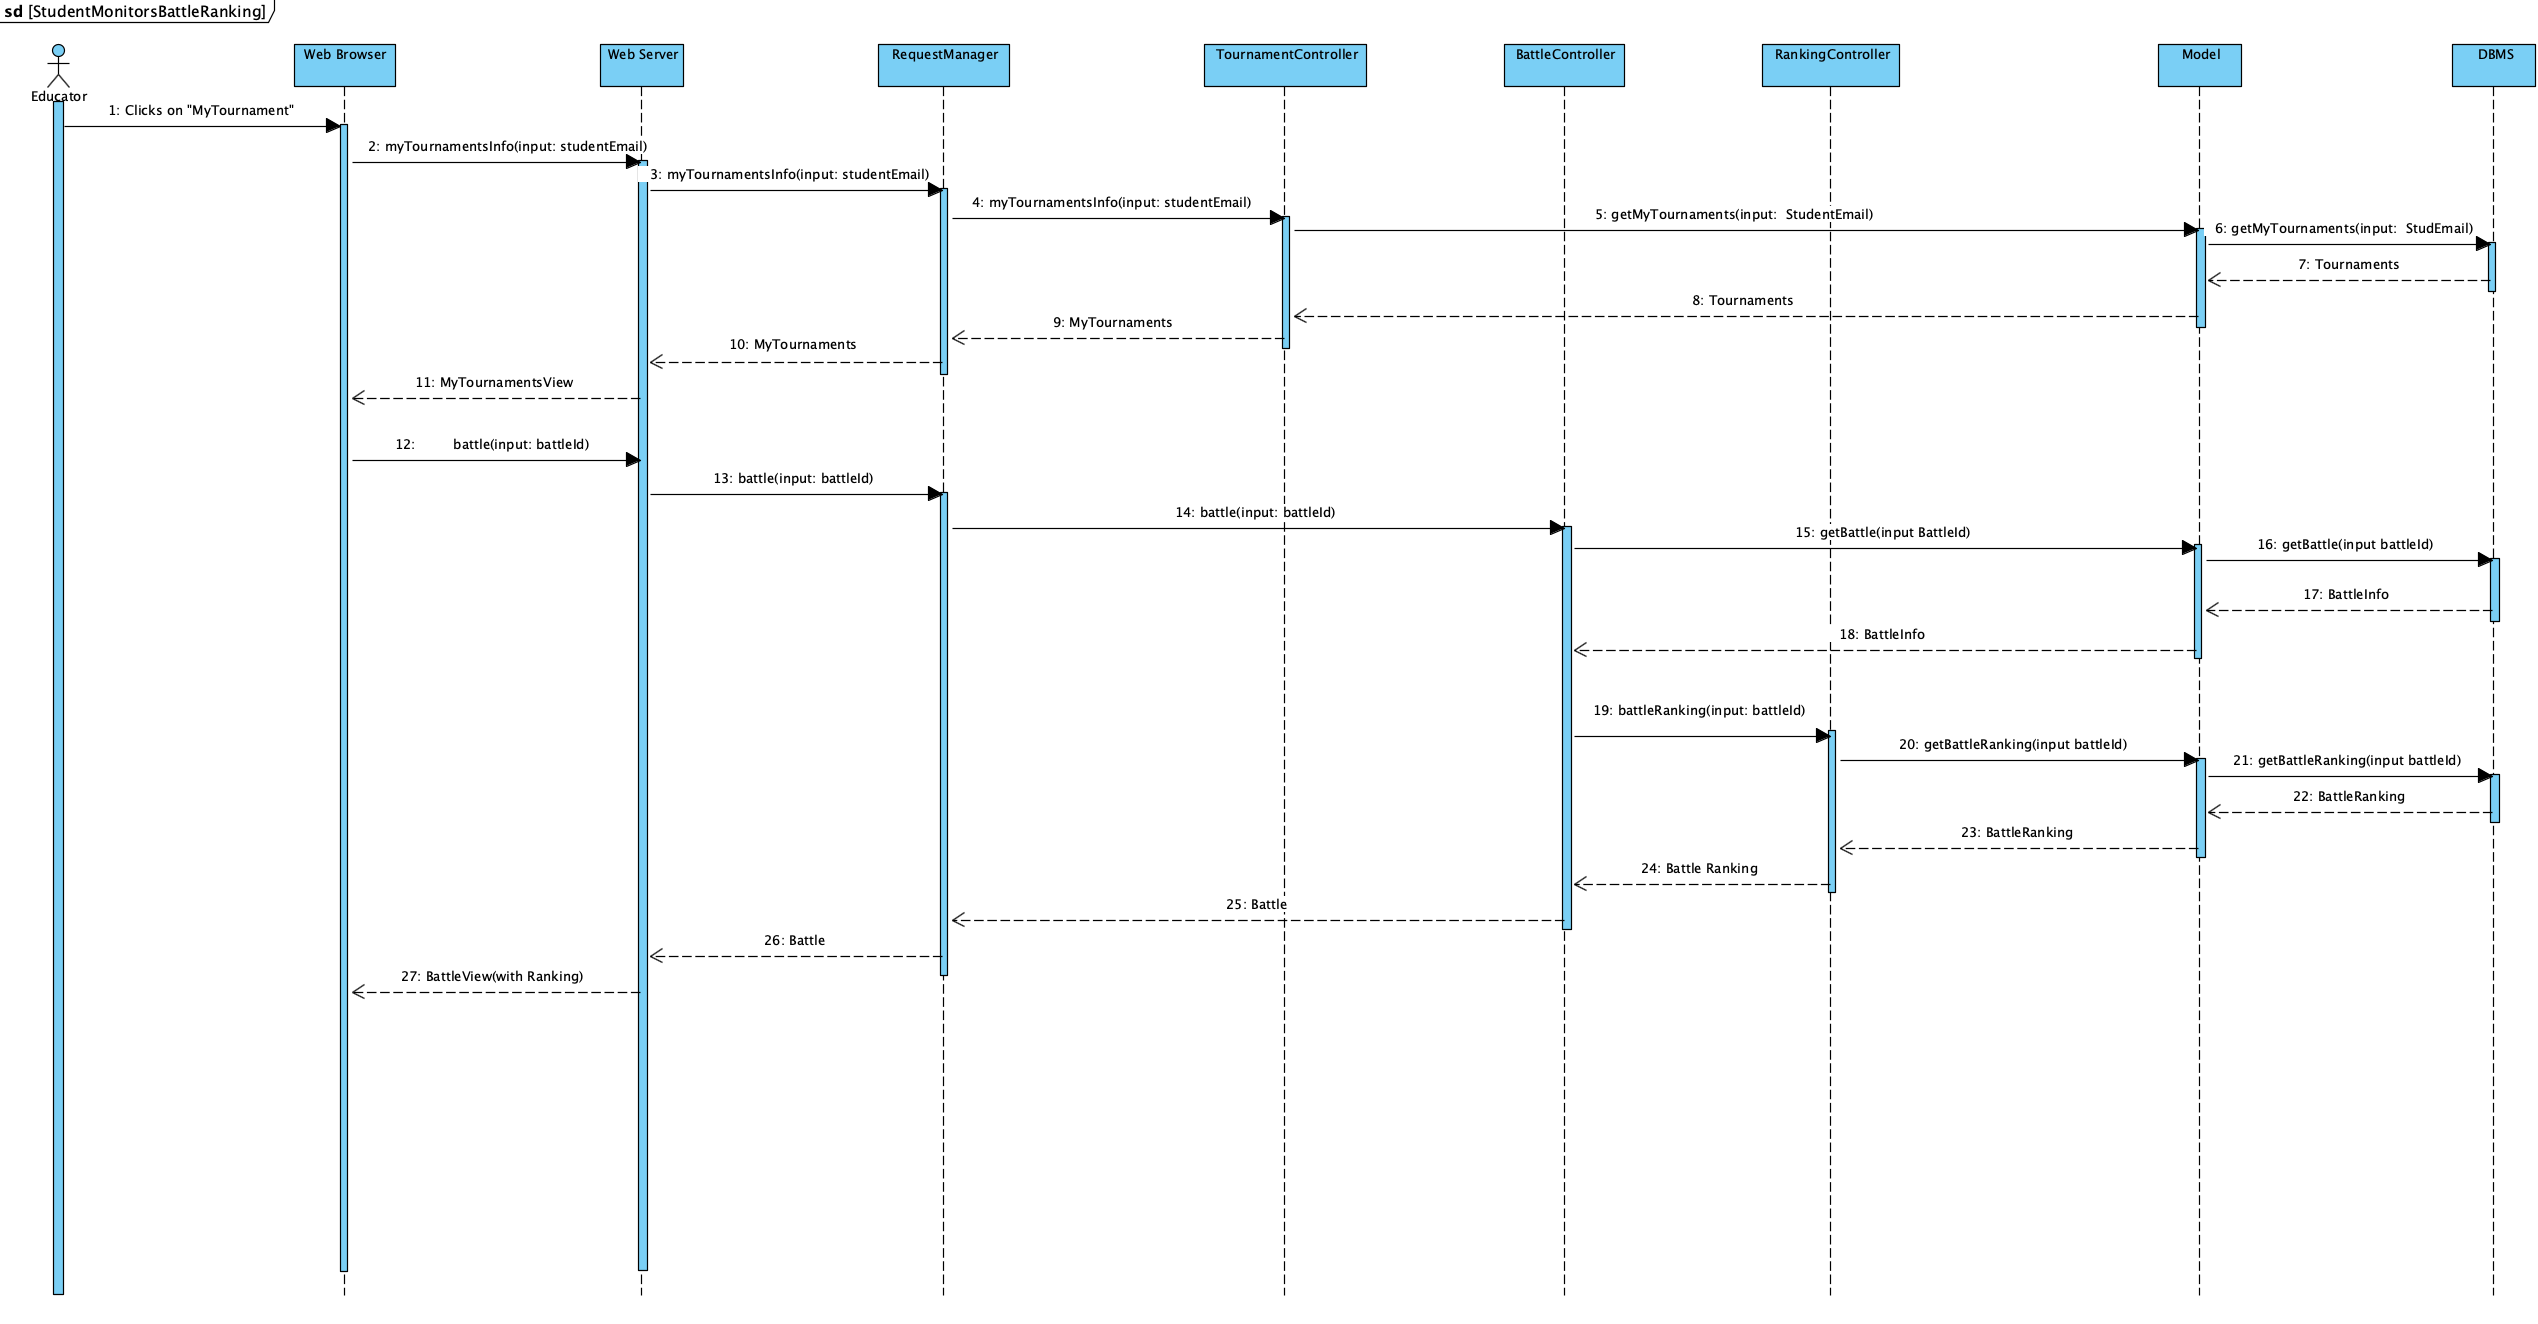
\includegraphics[width=1\linewidth]{SequenceDiagram/StudentMonitorsBattleRanking.png} 
  \caption{Student monitors battle ranking}
  \label{fig:immagine}
\end{figure}

\newpage
%% Educator monitors tournament ranking
\subsubsection{Educator monitors tournament ranking}

\begin{longtable}{|c| p{10cm}|}
    \hline
        ID & 15 \\
    \hline
        Name & Educator monitors tournament ranking \\
    \hline
        Actor & Educator \\
    \hline
        Entry Conditions & 
            \begin{itemize}
                \item The educator has logged into the system.
                \item The tournament of interest has been created, and the educator has the necessary permissions.
            \end{itemize}\\
    \hline
        Events Flow &   \begin{enumerate}
                            \item The educator, through the homepage, clicks on the "Tournament" section.
                            \item The system presents a control dashboard that displays the tournaments created by the educator or those for which they have permission to organize battles.
                            \item The educator clicks on "All Tournaments".
                            \item The system displays a page that includes all tournaments of the platform, even those for which the educator does not have permission to create battles.
                            \item The educator clicks on a specific tournament.
                            \item The system displays the dashboard containing battles for the selected tournament to the educator and the "Tournament ranking" button.
                            \item The educator clicks on "Tournament ranking".
                        \end{enumerate} \\
    \hline
        Exit Conditions &

            The system displays the tournament ranking containing various fields:
            \begin{itemize}
                                \item Student ID
                                \item Student Name
                                \item Student Surname
                                \item Student Score 
                            \end{itemize}
\\
    \hline
\end{longtable}


    \begin{figure}[H]
  %\centering
  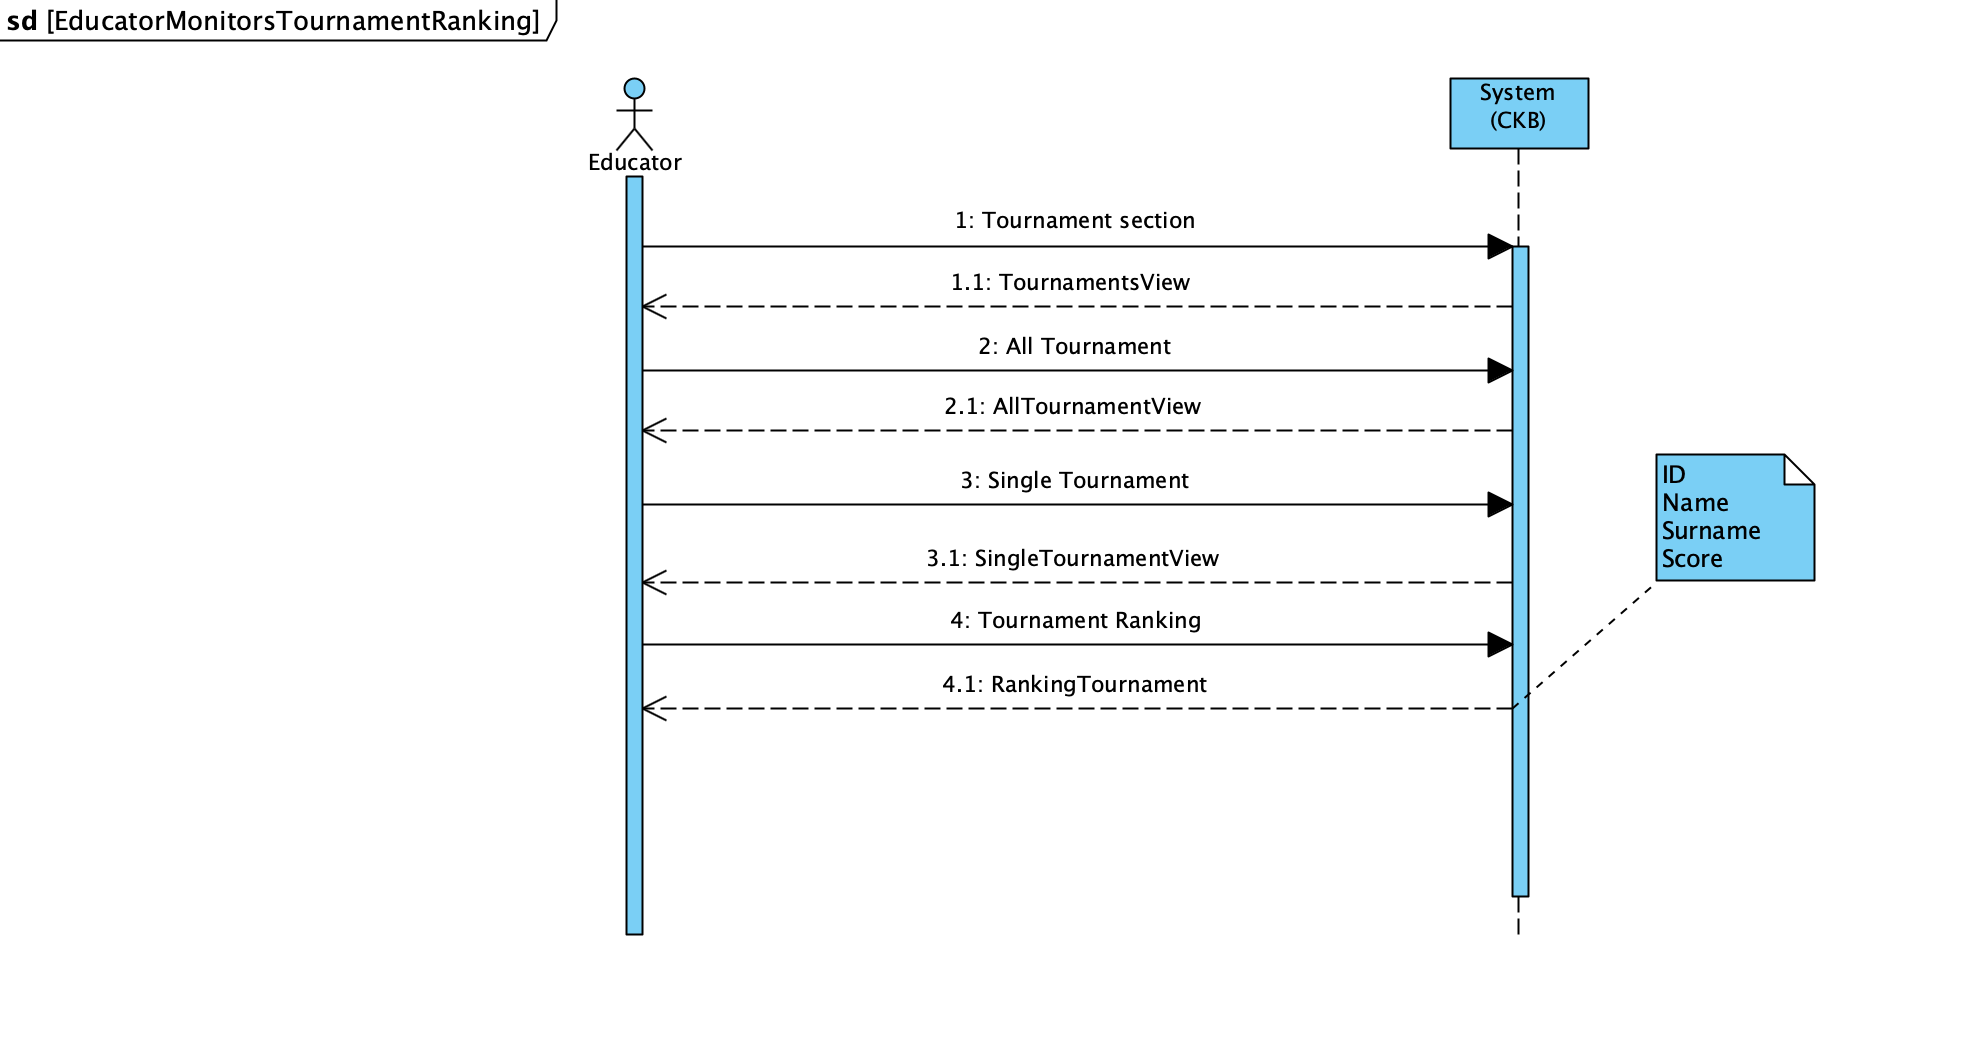
\includegraphics[width=1\linewidth]{SequenceDiagram/EducTournamentRanking.png} 
  \caption{Educator monitors tournament ranking}
  \label{fig:immagine}
\end{figure}

%% Student monitors tournament ranking
\subsubsection{Student monitors tournament ranking}

\begin{longtable}{|c| p{10cm}|}
    \hline
        ID & 16 \\
    \hline
        Name & Student monitors tournament ranking \\
    \hline
        Actor & Student \\
    \hline
        Entry Conditions & 
The student has logged into the system.
\\
    \hline
        Events Flow &   \begin{enumerate}
                            \item The student, through the homepage, clicks on the "Tournament" section.
                            \item The system presents a control dashboard that displays all the tournaments available on the platform.
                            \item The student clicks on a specific tournament.
                            \item The system displays the dashboard containing battles for the selected tournament to the student and the "Tournament ranking" button.
                            \item The student clicks on "Tournament ranking".
                        \end{enumerate} \\
    \hline
        Exit Conditions &

The system displays the tournament ranking containing various fields:
            \begin{itemize}
                                \item Student ID
                                \item Student Name
                                \item Student Surname
                                \item Student Score
                            \end{itemize}
\\
    \hline
\end{longtable}

    \begin{figure}[H]
  %\centering
  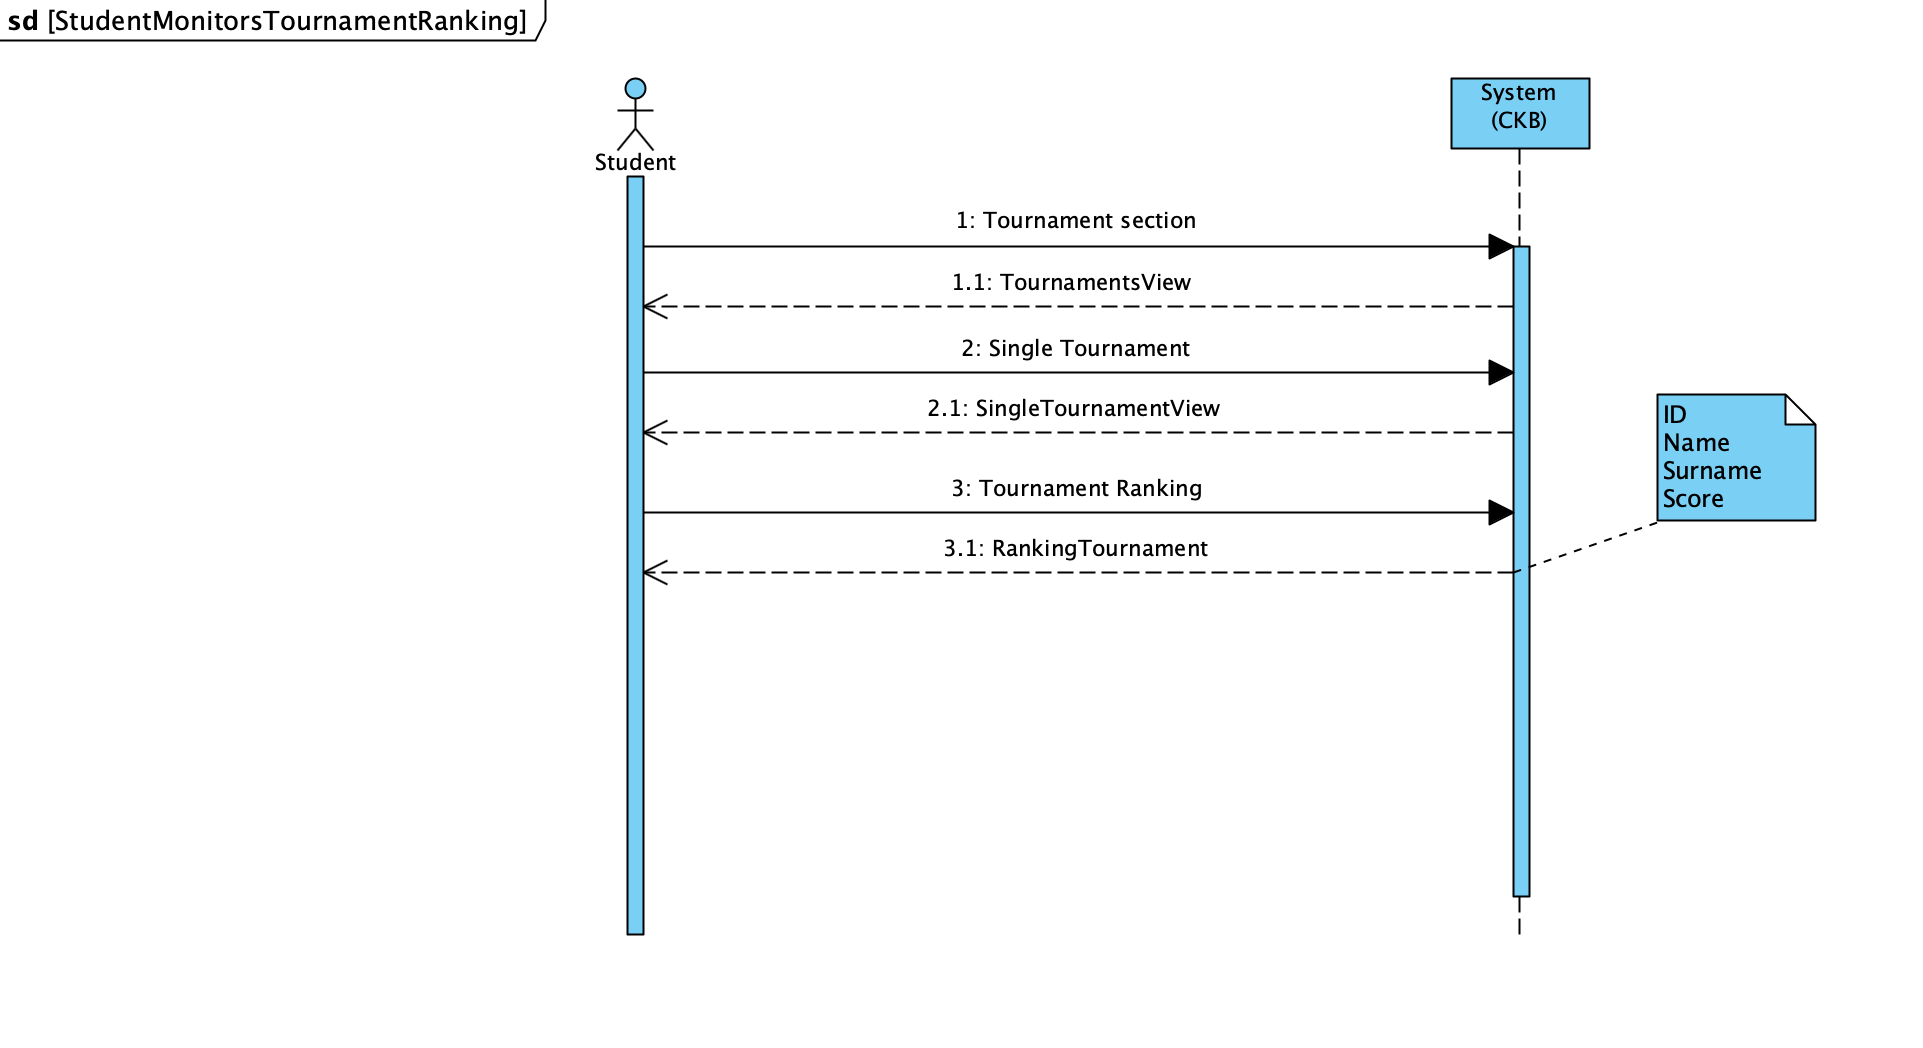
\includegraphics[width=1\linewidth]{SequenceDiagram/StudTournamentRanking.png} 
  \caption{Student monitors tournament ranking}
  \label{fig:immagine}
\end{figure}

\newpage
\subsubsection{Tournament Closure}
\begin{longtable}{|c| p{10cm}|}
        \hline
            ID & 17 \\
        \hline
            Name & Tournament Closure \\
        \hline
            Actor & Educator\\
        \hline
            Entry Conditions &
            \begin{itemize}
                \item The educator is logged into the system.
                \item The educator has created the tournament of interest.
            \end{itemize}\\
        \hline
            Events Flow &   \begin{enumerate}
                            \item The educator, through the homepage, clicks on the "Tournament" section.
                            \item The system presents a control dashboard that displays the tournaments created by the educator or those for which they have permission to organize battles.
                            \item The educator clicks on a specific tournament.
                            \item The system displays the dashboard containing battles for the selected tournament to the educator and the "Closure the tournament" button.
                            \item The educator selects "Close the tournament."
                            \item The system displays a warning message to confirm if the educator really intends to close the tournament.
                            \item The educator confirms the closure of the tournament, and the system checks if there are still open battles within the tournament.
                            \item The system changes the status of the same tournament from "Open" to "Closed."
                            \end{enumerate} \\
                            \hline
            Exit Conditions &
            The system updates the database and displays to the educator the message "Closure successfully completed.".
            \\
        \hline
         Exceptions &\begin{itemize}
             \item The educator responds to the warning sent by the platform about closing the tournament by clicking on "Cancel." Then, the platform displays the same page with a message explaining to the educator that the tournament closure operation has been canceled.
             \item The educator decides to close the tournament when there are still ongoing battles. So, the platform displays the same page with a message explaining to the educator that the tournament cannot be closed due to battles still in progress.
         \end{itemize} \\
             \hline
         
            
    \end{longtable}

    \begin{figure}[H]
  %\centering
  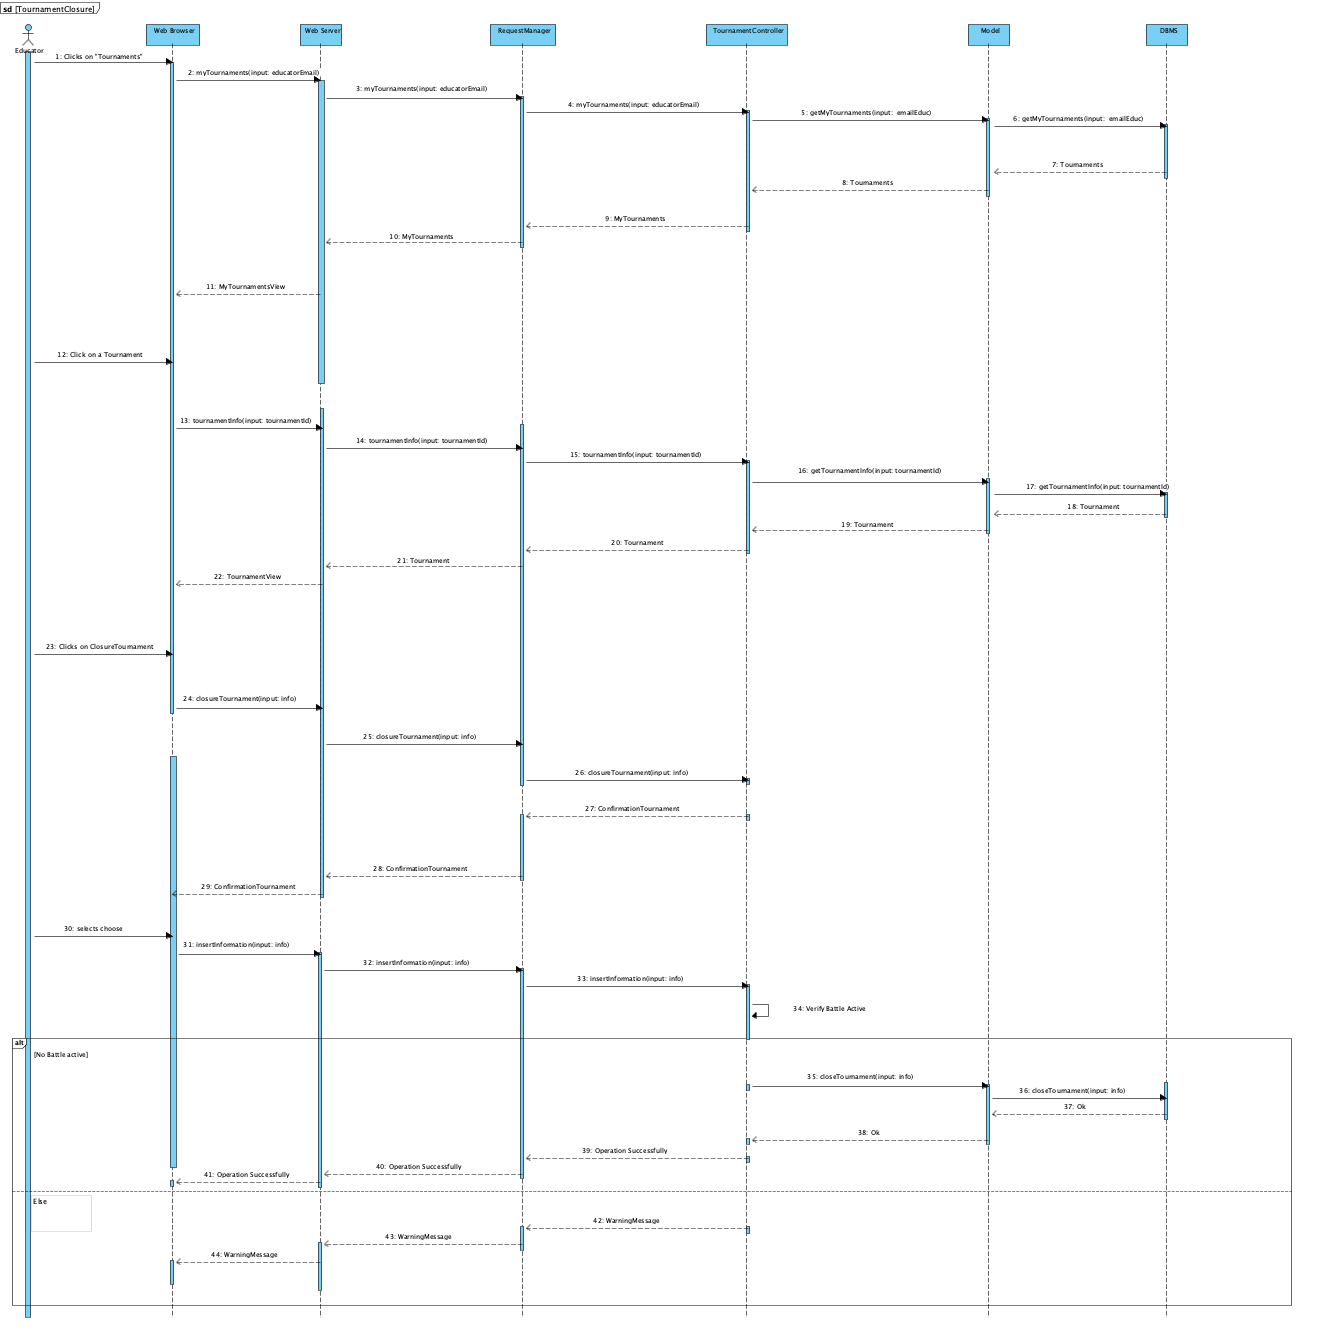
\includegraphics[width=1\linewidth]{SequenceDiagram/TournamentClosure.png} 
  \caption{Tournament Closure}
  \label{fig:immagine}
\end{figure}

\newpage
\subsubsection{Battle elimination}
\begin{longtable}{|c| p{10cm}|}
        \hline
            ID & 18 \\
        \hline
            Name & Tournament Closure \\
        \hline
            Actor & Educator\\
        \hline
            Entry Conditions &
            \begin{itemize}
                \item The educator is logged into the system.
                \item The educator has created the tournament of interest.
            \end{itemize}\\
        \hline
            Events Flow &   \begin{enumerate}
                            \item The educator, through the homepage, clicks on the "Tournament" section.
                            \item The system presents a control dashboard that displays the tournaments created by the educator or those for which they have permission to organize battles.
                            \item The educator clicks on a specific tournament.
                            \item The system displays the dashboard containing battles for the selected tournament to the educator and the "Closure the tournament" button.
                            \item The educator selects the battle of interest.
                            \item The system displays the BattleView.
                            \item The educator, before the registration deadline or after the termination of the battle, selects "Eliminate the battle".
                            \item The system displays a warning message to confirm if the educator really intends to eliminate the battle.
                            \item The educator confirms the elimination of the battle.
                            \end{enumerate} \\
                            \hline
            Exit Conditions &
            The system updates the database and displays to the educator the message "Closure successfully completed.".
            \\
        \hline
         Exceptions &
             The educator responds to the warning sent by the platform about the elimination of the tournament by clicking on "Cancel." Then, the platform displays the same page with a message explaining to the educator that the tournament closure operation has been canceled.
        \\
             \hline
         
            
    \end{longtable}


        \begin{figure}[H]
  %\centering
  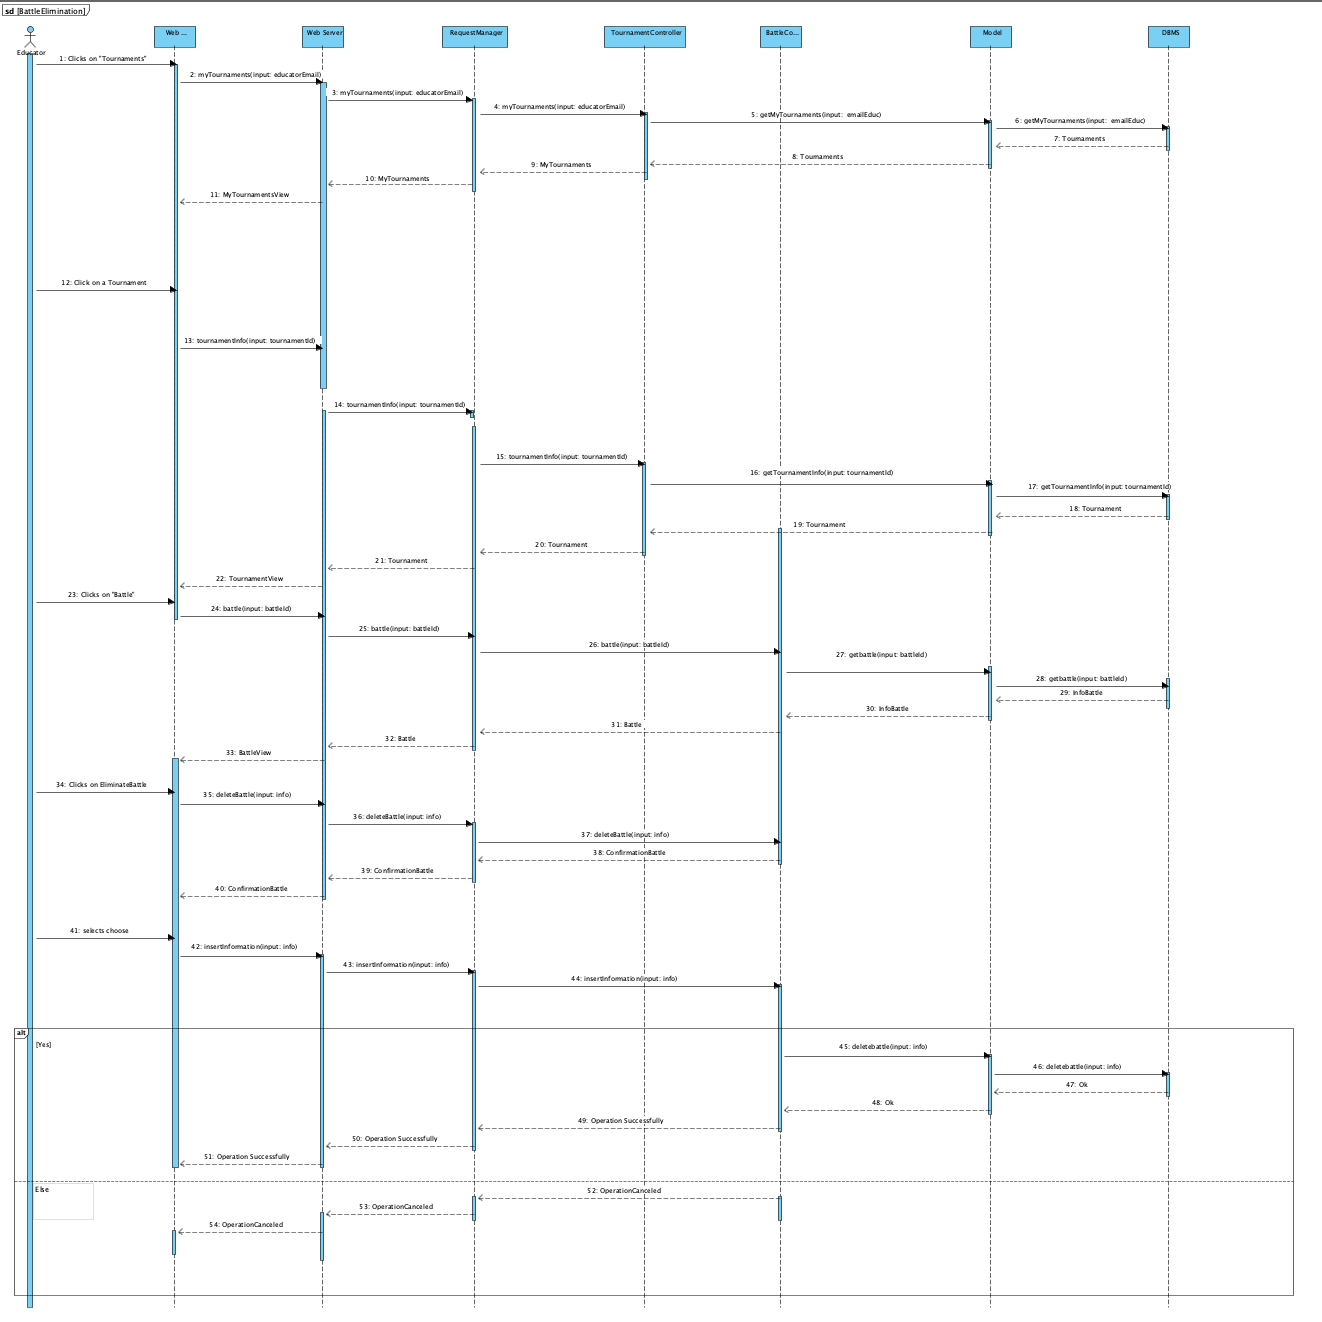
\includegraphics[width=1\linewidth]{SequenceDiagram/BattleElimination.png} 
  \caption{Battle elimination}
  \label{fig:immagine}
\end{figure}




\newpage
\subsubsection{Tournament Elimination}
\begin{longtable}{|c| p{10cm}|}
        \hline
            ID & 19 \\
        \hline
            Name & Tournament Elimination \\
        \hline
            Actor & Educator\\
        \hline
            Entry Conditions &
            \begin{itemize}
                \item The educator is logged into the system.
                \item The educator has either created the tournament of interest or possesses the necessary permissions to manage it.
            \end{itemize}\\
        \hline
            Events Flow &   \begin{enumerate}
                            \item The educator, through the homepage, clicks on the "Tournament" section.
                            \item The system presents a control dashboard that displays the tournaments created by the educator or those for which they have permission to organize battles.
                            \item The educator clicks on a specific tournament.
                            \item The system displays the dashboard containing battles for the selected tournament to the educator and also the "Delete tournament" button.
                            \item The educator selects "Delete tournament."
                            \item The system displays a warning message to confirm if the educator really intends to delete the tournament.
                            \item The educator confirms the elimination of the tournament, and the system checks if there are still open battles within the tournament.
                            \item The system delete the tournament.
                            \end{enumerate} \\
                            \hline
            Exit Conditions &
            The system updates the database and displays to the educator the message "Elimination successfully completed.".
            \\
        \hline
         Exceptions &\begin{itemize}
             \item The educator responds to the warning sent by the platform about eliminating the tournament by clicking on "Cancel." Then, the platform displays the same page with a message explaining to the educator that the tournament elimination operation has been canceled.
             \item The educator decides to delete the tournament when there are still ongoing battles. So, the platform displays the same page with a message explaining to the educator that the tournament cannot be deleted due to battles still in progress.
         \end{itemize} \\
             \hline
         
            
    \end{longtable}

        \begin{figure}[H]
  %\centering
  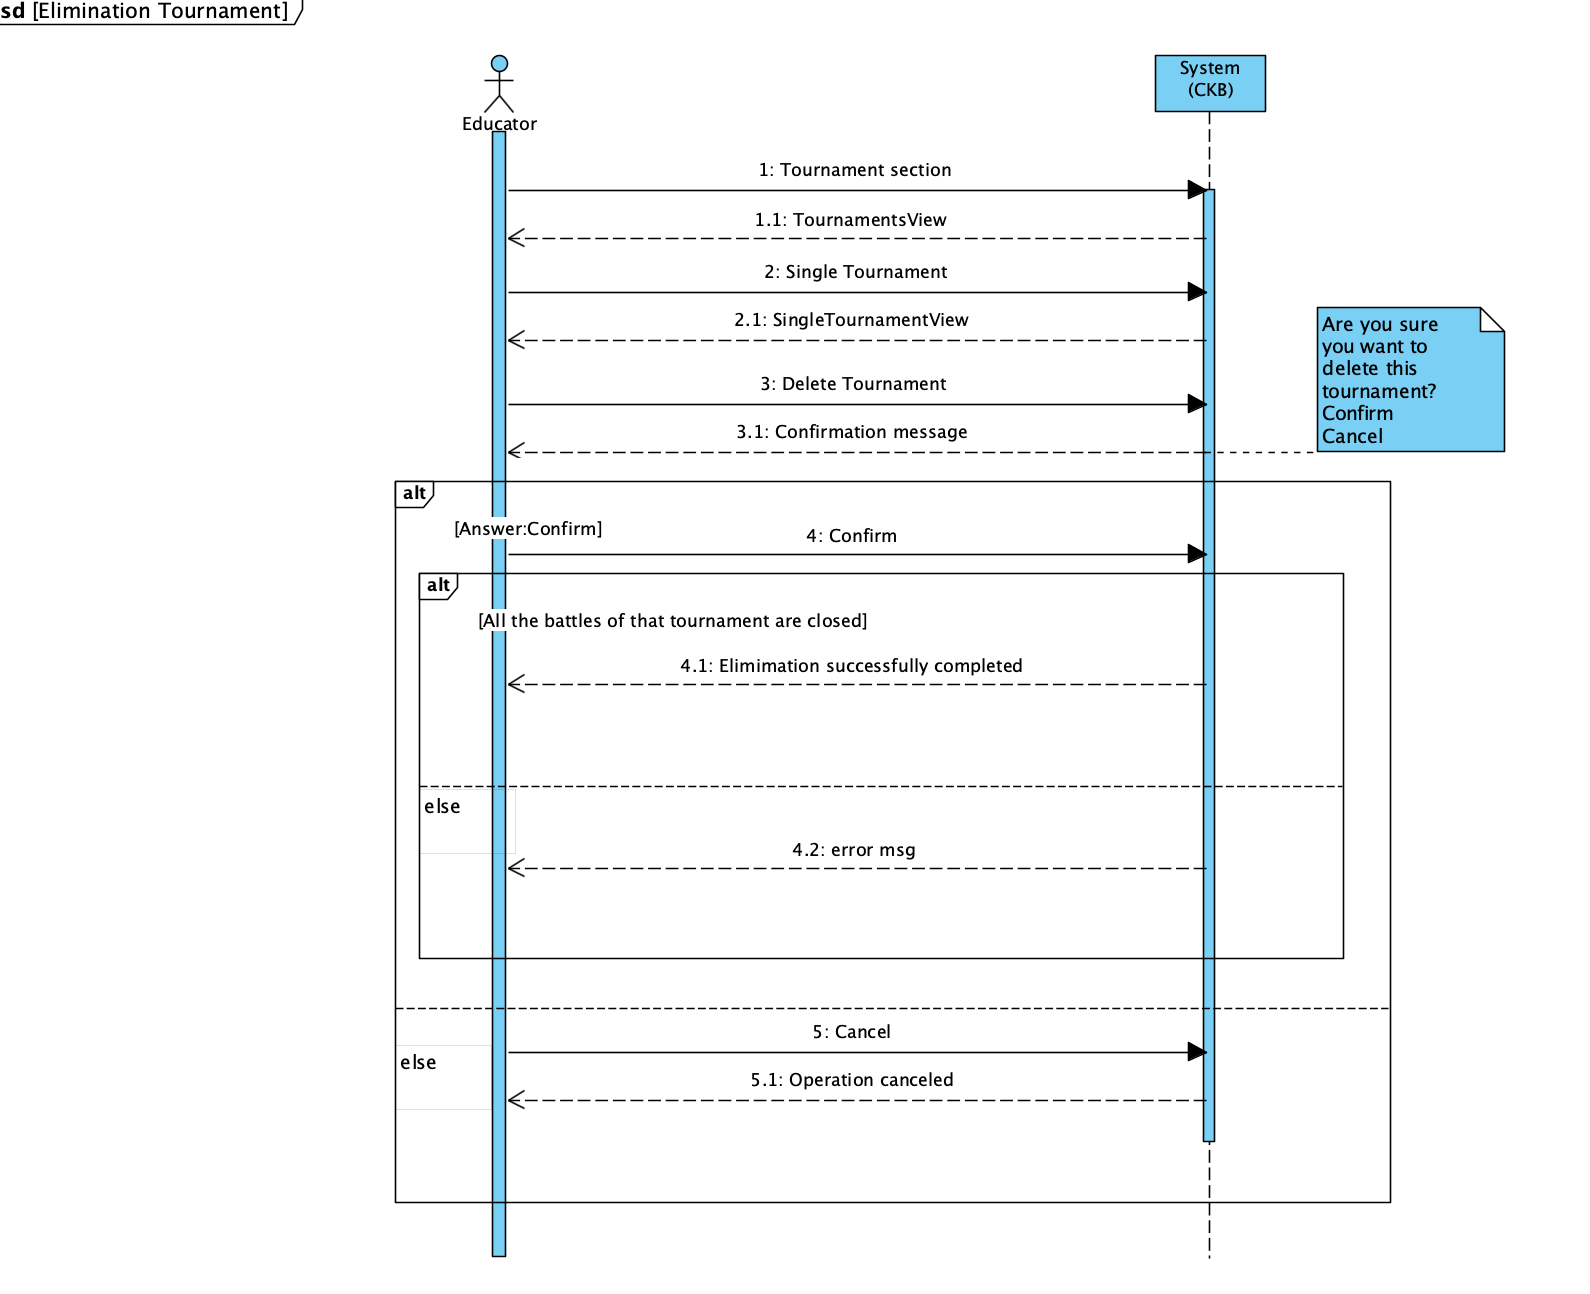
\includegraphics[width=1\linewidth]{SequenceDiagram/EliminationTournament.png} 
  \caption{Tournament Elimination}
  \label{fig:immagine}
\end{figure}
